\documentclass[12pt,oneside]{book}

\usepackage[scale=2]{ccicons}
\usepackage{enumitem}
\usepackage{multicol}
\usepackage[labelsep=period]{caption}
\usepackage[labelformat=simple,labelfont={}]{subcaption}
\usepackage{makecell}
%\usepackage{subcaption}
\usepackage{tabu}
\usepackage{pdiag}
\usepackage[table]{xcolor}
\usepackage{tikz}
\usetikzlibrary{arrows,automata,positioning}
\usepackage{rotating}
\usepackage[notextcomp]{kpfonts} 
\usepackage{graphicx}
\usepackage{eurosym}
\usepackage{amsfonts}
\usepackage{amsmath}
\usepackage{amssymb}
\usepackage{stmaryrd}
\usepackage{wasysym}
\usepackage{amsthm}
\usepackage[margin=1in]{geometry}
\usepackage[hang,flushmargin,symbol*]{footmisc}
\usepackage{color}
\definecolor{darkblue}{rgb}{0, 0, .6}
\definecolor{grey}{rgb}{.7, .7, .7}
\usepackage[breaklinks]{hyperref}
\hypersetup{
	colorlinks=true,
	linkcolor=darkblue,
	anchorcolor=darkblue,
	citecolor=darkblue,
	pagecolor=darkblue,
	urlcolor=darkblue,
	pdftitle={},
	pdfauthor={}
}

\usepackage{fancyhdr}
\pagestyle{fancy}
\lhead{\leftmark}
\chead{}
\rhead{}
\lfoot{}
\cfoot{}
\rfoot{}

\theoremstyle{definition}
\newtheorem{theorem}{Theorem}[chapter]
\newtheorem{acknowledgement}[theorem]{Acknowledgement}
\newtheorem{algorithm}[theorem]{Algorithm}
\newtheorem{axiom}[theorem]{Axiom}
\newtheorem{case}[theorem]{Case}
\newtheorem{claim}[theorem]{Claim}
\newtheorem{conclusion}[theorem]{Conclusion}
\newtheorem{condition}[theorem]{Condition}
\newtheorem{conjecture}[theorem]{Conjecture}
\newtheorem{corollary}[theorem]{Corollary}
\newtheorem{criterion}[theorem]{Criterion}
\newtheorem{definition}[theorem]{Definition}
\newtheorem{example}[theorem]{Example}
\newtheorem{exercise}[theorem]{Exercise}
\newtheorem{journal}[theorem]{Journal}
\newtheorem{lemma}[theorem]{Lemma}
\newtheorem{notation}[theorem]{Notation}
\newtheorem{problem}[theorem]{Problem}
\newtheorem{proposition}[theorem]{Proposition}
\newtheorem{remark}[theorem]{Remark}
\newtheorem{solution}[theorem]{Solution}
\newtheorem{summary}[theorem]{Summary}
\newtheorem{skeleton}[theorem]{Skeleton Proof}
\newtheorem{activity}[theorem]{Activity}
\newtheorem{intuitivedef}[theorem]{Intuitive Definition}

\newsavebox{\savepar}
\newenvironment{textbox}{\noindent\begin{lrbox}{\savepar}\begin{minipage}[c]{.98\textwidth}}{\end{minipage}\end{lrbox}\fcolorbox{black}{white}{\usebox{\savepar}}}

\newcommand{\dom}{\operatorname{Dom}}
\newcommand{\codom}{\operatorname{Codom}}
\newcommand{\range}{\operatorname{Rng}}
\newcommand{\Spin}{\operatorname{Spin}}
\newcommand{\lcm}{\operatorname{lcm}}

\renewcommand\thesubfigure{(\alph{subfigure})}

\begin{document}

\title{An Inquiry-Based Approach to Abstract Algebra}
\author{Dana C.~Ernst, PhD\\
Northern Arizona University}
\date{Fall 2017}

\maketitle
\thispagestyle{empty}

\noindent\copyright{ \the\year\ Dana C.~Ernst.  Some Rights Reserved.\\

\bigskip

\noindent This book is intended to be a task sequence for an undergraduate abstract algebra course that utilizes an inquiry-based learning (IBL) approach.  You can find the most up-to-date version of these notes on GitHub:
\begin{center}
\url{http://dcernst.github.io/IBL-AbstractAlgebra/}
\end{center}
I would be thrilled if you used these notes and improved them. If you make any modifications, you can either make a pull request on GitHub or submit the improvements via email.  You are also welcome to fork the source and modify the notes for your purposes as long as you maintain the license below.

\bigskip

\noindent This work is licensed under the Creative Commons Attribution-Share Alike 4.0 United States License.  You may copy, distribute, display, and perform this copyrighted work, but only if you give credit to Dana C.~Ernst, and all derivative works based upon it must be published under the Creative Commons Attribution-Share Alike 4.0 International License. Please attribute this work to Dana C.~Ernst, Mathematics Faculty at Northern Arizona University, \url{dana.ernst@nau.edu}. To view a copy of this license, visit
\begin{center}
\url{https://creativecommons.org/licenses/by-sa/4.0/}
\end{center}
or send a letter to Creative Commons, 171 Second Street, Suite 300, San Francisco, California, 94105, USA.}

\medskip

\begin{center}
\ccbysa
\end{center}

\noindent Here is a partial list of people (in alphabetical order by last name) that I need to thank for supplying content, advice, and feedback.
\begin{itemize}
\item \href{https://faculty.bentley.edu/details.asp?uname=ncarter}{Nathan Carter} (Bentley University). Nathan's excellent book \emph{Visual Group Theory} has had a huge impact on my approach to teaching abstract algebra.
\item \href{http://home.snc.edu/andershendrickson/}{Anders Hendrickson} (St.~Norbert College). Anders is the original author of the content in Appendix~\ref{appendix:elements_of_style}: Elements of Style for Proofs. The current version in Appendix~\ref{appendix:elements_of_style} is a result of modifications made by myself with some suggestions from Dave Richeson.
\item \href{http://users.dickinson.edu/~richesod/}{Dave Richeson} (Dickinson College). Dave is responsible for much of the content in Appendix~\ref{appendix:fancy_math_terms}: Fancy Mathematical Terms and Appendix~\ref{appendix:definitions}: Definitions in Mathematics. 
\item \href{http://webpages.csus.edu/wiscons/}{Josh Wiscons} (CSU Sacremento) and \href{http://emp.byui.edu/woodruffb/}{Ben Woodruff} (BYU Idaho). Josh and Ben were instrumental the development of these notes in their early stages of development.
\end{itemize}

\tableofcontents
\thispagestyle{empty}

\chapter{Introduction}

\begin{section}{What is Abstract Algebra?}

Abstract algebra is the subject area of mathematics that studies algebraic structures, such as groups, rings, fields, modules, vector spaces, and algebras. This course is an introduction to abstract algebra. We will spend most of our time studying groups. Group theory is the study of symmetry, and is one of the most beautiful areas in all of mathematics. It arises in puzzles, visual arts, music, nature, the physical and life sciences, computer science, cryptography, and of course, throughout mathematics. This course will cover the basic concepts of group theory, and a special effort will be made to emphasize the intuition behind the concepts and motivate the subject matter.  In the last few weeks of the semester, we will also introduce rings and fields.
\epigraph{The mathematician does not study pure mathematics because it is useful; he studies it because he delights in it, and he delights in it because it is beautiful.}{\emph{Henri Poincar\'e}}

\end{section}

\begin{section}{An Inquiry-Based Approach}

This is not a lecture-oriented class or one in which mimicking prefabricated examples will lead you to success. You will be expected to work actively to construct your own understanding of the topics at hand with the readily available help of me and your classmates. Many of the concepts you learn and problems you work on will be new to you and ask you to stretch your thinking. You will experience \emph{frustration} and \emph{failure} before you experience \emph{understanding}. This is part of the normal learning process. If you are doing things well, you should be confused at different points in the semester. The material is too rich for a human being to completely understand it immediately. Your viability as a professional in the modern workforce depends on your ability to embrace this learning process and make it work for you.

\epigraph{Don't fear failure.  Not failure, but low aim, is the crime. In great attempts it is glorious even to fail.}{\emph{Bruce Lee}}

In order to promote a more active participation in your learning, we will incorporate ideas from an educational philosophy called inquiry-based learning (IBL).  Loosely speaking, IBL is a student-centered method of teaching mathematics that engages students in sense-making activities.  Students are given tasks requiring them to solve problems, conjecture, experiment, explore, create, and communicate.  Rather than showing facts or a clear, smooth path to a solution, the instructor guides and mentors students via well-crafted problems through an adventure in mathematical discovery.  According to \href{https://www.colorado.edu/eer/sites/default/files/attached-files/laursenrasmussencommentaryauthorversion0219.pdf}{Laursen and Rasmussen (2019)}, the Four Pillars of IBL are:
\begin{itemize}
\item Students engage deeply with coherent and meaningful mathematical tasks.
\item Students collaboratively process mathematical ideas.
\item Instructors inquire into student thinking.
\item Instructors foster equity in their design and facilitation choices.
\end{itemize}

Much of the course will be devoted to students presenting their proposed solutions or proofs on the board and a significant portion of your grade will be determined by how much mathematics you produce.  I use the word \emph{produce} because I believe that the best way to learn mathematics is by doing mathematics.  Someone cannot master a musical instrument or a martial art by simply watching, and in a similar fashion, you cannot master mathematics by simply watching; you must do mathematics!

In any act of creation, there must be room for experimentation, and thus allowance for mistakes, even failure. A key goal of our community is that we support each other---sharpening each other's thinking but also bolstering each other's confidence---so that we can make failure a productive experience. Mistakes are inevitable, and they should not be an obstacle to further progress. It's normal to struggle and be confused as you work through new material. Accepting that means you can keep working even while feeling stuck, until you overcome and reach even greater accomplishments.

\epigraph{You will become clever through your mistakes.}{\emph{German Proverb}}

Furthermore, it is important to understand that solving genuine problems is difficult and takes time.  You shouldn't expect to complete each problem in 10 minutes or less.  Sometimes, you might have to stare at the problem for an hour before even understanding how to get started.

In this course, everyone will be required to
\begin{itemize}
\item read and interact with course notes and textbook on your own;
\item write up quality solutions/proofs to assigned problems;
\item present solutions/proofs on the board to the rest of the class;
\item participate in discussions centered around a student's presented solution/proof;
\item call upon your own prodigious mental faculties to respond in flexible, thoughtful, and creative ways to problems that may seem unfamiliar on first glance.
\end{itemize}
As the semester progresses, it should become clear to you what the expectations are.

\epigraph{Tell me and I forget, teach me and I may remember, involve me and I learn.}{\emph{Benjamin Franklin}}

\end{section}

\begin{section}{Rights of the Learner}
As a student in this class, you have the right:
\begin{enumerate}
\item to be confused,
\item to make a mistake and to revise your thinking,
\item to speak, listen, and be heard, and
\item to enjoy doing mathematics.
\end{enumerate}

\epigraph{You may encounter many defeats, but you must not be defeated.}{\emph{Maya Angelou}}
	
\end{section}

\begin{section}{Structure of the Notes}

As you read the notes, you will be required to digest the material in a meaningful way.  It is your responsibility to read and understand new definitions and their related concepts.  However, you will be supported in this sometimes difficult endeavor. In addition, you will be asked to complete problems aimed at solidifying your understanding of the material.  Most importantly, you will be asked to make conjectures, produce counterexamples, and prove theorems.

The items labeled as \textbf{Definition} and \textbf{Example} are meant to be read and digested.  However, the items labeled as \textbf{Problem}, \textbf{Theorem}, and \textbf{Corollary} require action on your part.  Items labeled as \textbf{Problem} are sort of a mixed bag. Some Problems are computational in nature and aimed at improving your understanding of a particular concept while others ask you to provide a counterexample for a statement if it is false or to provide a proof if the statement is true. Items with the \textbf{Theorem} and \textbf{Corollary} designation are mathematical facts and the intention is for you to produce a valid proof of the given statement.  The main difference between a \textbf{Theorem} and a \textbf{Corollary} is that corollaries are typically statements that follow quickly from a previous theorem.  In general, you should expect corollaries to have very short proofs.  However, that doesn't mean that you can't produce a more lengthy yet valid proof of a corollary.

It is important to point out that there are very few examples in the notes.  This is intentional.  One of the goals of the items labeled as \textbf{Problem} is for you to produce the examples.

Lastly, there are many situations where you will want to refer to an earlier definition, problem, theorem, or corollary.  In this case, you should reference the statement by number.  For example, you might write something like, ``By Theorem~\ref{thm:order_element_divides_group_order}, we see that\ldots."

\end{section}

\begin{section}{Some Minimal Guidance}
Especially in the opening sections, it won't be clear what facts from your prior experience in mathematics we are ``allowed" to use.  Unfortunately, addressing this issue is difficult and is something we will sort out along the way.  However, in general, here are some minimal guidelines to keep in mind.  

First, there are times when we will need to do some basic algebraic manipulations.  You should feel free to do this whenever the need arises.  But you should show sufficient work along the way.  You do not need to write down justifications for basic algebraic manipulations (e.g., adding 1 to both sides of an equation, adding and subtracting the same amount on the same side of an equation, adding like terms, factoring, basic simplification, etc.).  

On the other hand, you do need to make explicit justification of the logical steps in a proof.  When necessary, you should cite a previous definition, theorem, etc. by number.

Unlike the experience many of you had writing proofs in geometry, our proofs will be written in complete sentences.  You should break sections of a proof into paragraphs and use proper grammar.  There are some pedantic conventions for doing this that I will point out along the way.  Initially, this will be an issue that most students will struggle with, but after a few weeks everyone will get the hang of it.

Ideally, you should rewrite the statements of theorems before you start the proof.  Moreover, for your sake and mine, you should label the statement with the appropriate number.  I will expect you to indicate where the proof begins by writing ``\emph{Proof.}" at the beginning.  Also, we will conclude our proofs with the standard ``proof box" (i.e., $\square$ or $\blacksquare$), which is typically right-justified.

Lastly, every time you write a proof, you need to make sure that you are making your assumptions crystal clear.  Sometimes there will be some implicit assumptions that we can omit, but at least in the beginning, you should get in the habit of stating your assumptions up front.  Typically, these statements will start off ``Assume\ldots" or ``Let\ldots".  

This should get you started.  We will discuss more as the semester progresses.  Now, go have fun and kick some butt!

\epigraph{If you want to sharpen a sword, you have to remove a little metal.}{\emph{Unknown}}

\end{section}
\chapter{An Intuitive Approach to Groups}
\label{chapter:intuitive_approach_groups}
\thispagestyle{empty}

One of the major topics of this course is \textbf{groups}.  The area of mathematics that is concerned with groups is called \textbf{group theory}. Loosely speaking, group theory is the study of symmetry, and in my opinion is one of the most beautiful areas in all of mathematics. It arises in puzzles, visual arts, music, nature, the physical and life sciences, computer science, cryptography, and of course, throughout mathematics.

Instead of starting with an abstract formal definition, we will begin our study of groups by developing some intuition about what groups actually are.  To get started, we will be exploring the game Spinpossible\texttrademark, which is a free game that is available for iOS and Android devices. Alternatively, you can just play the game in any modern web browser (\url{https://spinpossible.com}).  The game is played on a $3\times 3$ board of scrambled tiles numbered 1 to 9, each of which may be right-side-up or up-side-down. The objective of the game is to return the board to the standard configuration where tiles are arranged in numerical order and right-side-up. This is accomplished by a sequence of ``spins", where a spin consists of rotating an $m\times n$ subrectangle by 180$^\circ$. The goal is to minimize the number of spins used.  The following figure depicts a scrambled board on the left and the solved board on the right.  The sequence of arrows is used to denote some sequence of spins that transforms the scrambled board into the solved board.

\begin{center}
\begin{tabular}{c}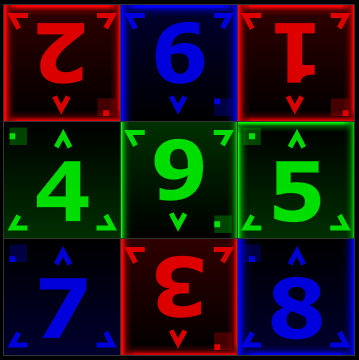
\includegraphics[width=1.5in]{scramble1.PNG}\end{tabular}
{\large $\xrightarrow{?} \cdots \xrightarrow{?}$}
\begin{tabular}{c}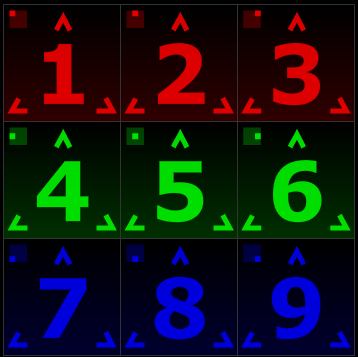
\includegraphics[width=1.5in]{scramble4.PNG}\end{tabular}
\end{center}

\begin{example}\label{ex:spinpossible}
Let's play with an example.  Suppose we start with the following scrambled board.

\begin{center}
\begin{tikzpicture}[every node/.style={minimum size=.65cm}]
  \node [draw] (1) {\rotatebox{180}{$\underline{2}$}};
  \node [draw, right=0cm of 1] (2) {\rotatebox{180}{$\underline{9}$}};
  \node [draw, right=0cm of 2] (3) {\rotatebox{180}{$\underline{1}$}};
  \node [draw, below=0cm of 1] (4) {$\underline{4}$};
  \node [draw, right=0cm of 4] (5) {\rotatebox{180}{$\underline{6}$}};
  \node [draw, right=0cm of 5] (6) {$\underline{5}$};
  \node [draw, below=0cm of 4] (7) {$\underline{7}$};
  \node [draw, right=0cm of 7] (8) {\rotatebox{180}{$\underline{3}$}};
  \node [draw, right=0cm of 8] (9) {$\underline{8}$};
\end{tikzpicture}
\end{center}

\noindent The underlines on the numbers are meant to help us tell whether a tile is right-side-up or up-side-down.  Our goal is to use a sequence of spins to unscramble the board.  Before we get started, let's agree on some conventions.  When we refer to tile $n$, we mean the actual tile that is labeled by the number $n$ regardless of its position and orientation on the board.  On the other hand, position $n$ will refer to the position on the board that tile $n$ is supposed to be in when the board has been unscrambled.  For example, in the board above, tile 1 is in position 3 and tile 7 happens to be in position 7.  

It turns out that there are multiple ways to unscramble this board., but I have one particular sequence in mind.  First, let's spin the rectangle determined by the two rightmost columns.  Here's what we get.  I've shaded the subrectangle that we are spinning.

\begin{center}
\begin{tabular}{c}
\begin{tikzpicture}[every node/.style={minimum size=.65cm}]
  \node [draw] (1) {\rotatebox{180}{$\underline{2}$}};
  \node [draw, fill=blue!40, right=0cm of 1] (2) {\rotatebox{180}{$\underline{9}$}};
  \node [draw, fill=blue!40, right=0cm of 2] (3) {\rotatebox{180}{$\underline{1}$}};
  \node [draw, below=0cm of 1] (4) {$\underline{4}$};
  \node [draw, fill=blue!40, right=0cm of 4] (5) {\rotatebox{180}{$\underline{6}$}};
  \node [draw, fill=blue!40, right=0cm of 5] (6) {$\underline{5}$};
  \node [draw, below=0cm of 4] (7) {$\underline{7}$};
  \node [draw, fill=blue!40, right=0cm of 7] (8) {\rotatebox{180}{$\underline{3}$}};
  \node [draw, fill=blue!40, right=0cm of 8] (9) {$\underline{8}$};
\end{tikzpicture}
\end{tabular}
%
{\large $\rightarrow$}
%
\begin{tabular}{c}
\begin{tikzpicture}[every node/.style={minimum size=.65cm}]
  \node [draw] (1) {\rotatebox{180}{$\underline{2}$}};
  \node [draw, right=0cm of 1] (2) {\rotatebox{180}{$\underline{8}$}};
  \node [draw, right=0cm of 2] (3) {$\underline{3}$};
  \node [draw, below=0cm of 1] (4) {$\underline{4}$};
  \node [draw, right=0cm of 4] (5) {\rotatebox{180}{$\underline{5}$}};
  \node [draw, right=0cm of 5] (6) {$\underline{6}$};
  \node [draw, below=0cm of 4] (7) {$\underline{7}$};
  \node [draw, right=0cm of 7] (8) {$\underline{1}$};
  \node [draw, right=0cm of 8] (9) {$\underline{9}$};
\end{tikzpicture}
\end{tabular}
\end{center}

\noindent Okay, now let's spin the middle column.

\begin{center}
\begin{tabular}{c}
\begin{tikzpicture}[every node/.style={minimum size=.65cm}]
  \node [draw] (1) {\rotatebox{180}{$\underline{2}$}};
  \node [draw, fill=blue!40, right=0cm of 1] (2) {\rotatebox{180}{$\underline{8}$}};
  \node [draw, right=0cm of 2] (3) {$\underline{3}$};
  \node [draw, below=0cm of 1] (4) {$\underline{4}$};
  \node [draw, fill=blue!40, right=0cm of 4] (5) {\rotatebox{180}{$\underline{5}$}};
  \node [draw, right=0cm of 5] (6) {$\underline{6}$};
  \node [draw, below=0cm of 4] (7) {$\underline{7}$};
  \node [draw, fill=blue!40, right=0cm of 7] (8) {$\underline{1}$};
  \node [draw, right=0cm of 8] (9) {$\underline{9}$};
\end{tikzpicture}
\end{tabular}
%
{\large $\rightarrow$}
%
\begin{tabular}{c}
\begin{tikzpicture}[every node/.style={minimum size=.65cm}]
  \node [draw] (1) {\rotatebox{180}{$\underline{2}$}};
  \node [draw, right=0cm of 1] (2) {\rotatebox{180}{$\underline{1}$}};
  \node [draw, right=0cm of 2] (3) {$\underline{3}$};
  \node [draw, below=0cm of 1] (4) {$\underline{4}$};
  \node [draw, right=0cm of 4] (5) {$\underline{5}$};
  \node [draw, right=0cm of 5] (6) {$\underline{6}$};
  \node [draw, below=0cm of 4] (7) {$\underline{7}$};
  \node [draw, right=0cm of 7] (8) {$\underline{8}$};
  \node [draw, right=0cm of 8] (9) {$\underline{9}$};
\end{tikzpicture}
\end{tabular}
\end{center}

\noindent Hopefully, you can see that we are really close to unscrambling the board.  All we need to do is spin the rectangle determined by the tiles in positions 1 and 2.

\begin{center}
\begin{tabular}{c}
\begin{tikzpicture}[every node/.style={minimum size=.65cm}]
  \node [draw, fill=blue!40] (1) {\rotatebox{180}{$\underline{2}$}};
  \node [draw, fill=blue!40, right=0cm of 1] (2) {\rotatebox{180}{$\underline{1}$}};
  \node [draw, right=0cm of 2] (3) {$\underline{3}$};
  \node [draw, below=0cm of 1] (4) {$\underline{4}$};
  \node [draw, right=0cm of 4] (5) {$\underline{5}$};
  \node [draw, right=0cm of 5] (6) {$\underline{6}$};
  \node [draw, below=0cm of 4] (7) {$\underline{7}$};
  \node [draw, right=0cm of 7] (8) {$\underline{8}$};
  \node [draw, right=0cm of 8] (9) {$\underline{9}$};
\end{tikzpicture}
\end{tabular}
%
{\large $\rightarrow$}
%
\begin{tabular}{c}
\begin{tikzpicture}[every node/.style={minimum size=.65cm}]
  \node [draw] (1) {$\underline{1}$};
  \node [draw, right=0cm of 1] (2) {$\underline{2}$};
  \node [draw, right=0cm of 2] (3) {$\underline{3}$};
  \node [draw, below=0cm of 1] (4) {$\underline{4}$};
  \node [draw, right=0cm of 4] (5) {$\underline{5}$};
  \node [draw, right=0cm of 5] (6) {$\underline{6}$};
  \node [draw, below=0cm of 4] (7) {$\underline{7}$};
  \node [draw, right=0cm of 7] (8) {$\underline{8}$};
  \node [draw, right=0cm of 8] (9) {$\underline{9}$};
\end{tikzpicture}
\end{tabular}
\end{center}

\noindent Putting all of our moves together, here is what we have.

\begin{center}
\begin{tabular}{c}
\begin{tikzpicture}[every node/.style={minimum size=.65cm}]
  \node [draw] (1) {\rotatebox{180}{$\underline{2}$}};
  \node [draw, fill=blue!40, right=0cm of 1] (2) {\rotatebox{180}{$\underline{9}$}};
  \node [draw, fill=blue!40, right=0cm of 2] (3) {\rotatebox{180}{$\underline{1}$}};
  \node [draw, below=0cm of 1] (4) {$\underline{4}$};
  \node [draw, fill=blue!40, right=0cm of 4] (5) {\rotatebox{180}{$\underline{6}$}};
  \node [draw, fill=blue!40, right=0cm of 5] (6) {$\underline{5}$};
  \node [draw, below=0cm of 4] (7) {$\underline{7}$};
  \node [draw, fill=blue!40, right=0cm of 7] (8) {\rotatebox{180}{$\underline{3}$}};
  \node [draw, fill=blue!40, right=0cm of 8] (9) {$\underline{8}$};
\end{tikzpicture}
\end{tabular}
%
{\large $\rightarrow$}
%
\begin{tabular}{c}
\begin{tikzpicture}[every node/.style={minimum size=.65cm}]
  \node [draw] (1) {\rotatebox{180}{$\underline{2}$}};
  \node [draw, fill=blue!40, right=0cm of 1] (2) {\rotatebox{180}{$\underline{8}$}};
  \node [draw, right=0cm of 2] (3) {$\underline{3}$};
  \node [draw, below=0cm of 1] (4) {$\underline{4}$};
  \node [draw, fill=blue!40, right=0cm of 4] (5) {\rotatebox{180}{$\underline{5}$}};
  \node [draw, right=0cm of 5] (6) {$\underline{6}$};
  \node [draw, below=0cm of 4] (7) {$\underline{7}$};
  \node [draw, fill=blue!40, right=0cm of 7] (8) {$\underline{1}$};
  \node [draw, right=0cm of 8] (9) {$\underline{9}$};
\end{tikzpicture}
\end{tabular}
%
{\large $\rightarrow$}
%
\begin{tabular}{c}
\begin{tikzpicture}[every node/.style={minimum size=.65cm}]
  \node [draw, fill=blue!40] (1) {\rotatebox{180}{$\underline{2}$}};
  \node [draw, fill=blue!40, right=0cm of 1] (2) {\rotatebox{180}{$\underline{1}$}};
  \node [draw, right=0cm of 2] (3) {$\underline{3}$};
  \node [draw, below=0cm of 1] (4) {$\underline{4}$};
  \node [draw, right=0cm of 4] (5) {$\underline{5}$};
  \node [draw, right=0cm of 5] (6) {$\underline{6}$};
  \node [draw, below=0cm of 4] (7) {$\underline{7}$};
  \node [draw, right=0cm of 7] (8) {$\underline{8}$};
  \node [draw, right=0cm of 8] (9) {$\underline{9}$};
\end{tikzpicture}
\end{tabular}
%
{\large $\rightarrow$}
%
\begin{tabular}{c}
\begin{tikzpicture}[every node/.style={minimum size=.65cm}]
  \node [draw] (1) {$\underline{1}$};
  \node [draw, right=0cm of 1] (2) {$\underline{2}$};
  \node [draw, right=0cm of 2] (3) {$\underline{3}$};
  \node [draw, below=0cm of 1] (4) {$\underline{4}$};
  \node [draw, right=0cm of 4] (5) {$\underline{5}$};
  \node [draw, right=0cm of 5] (6) {$\underline{6}$};
  \node [draw, below=0cm of 4] (7) {$\underline{7}$};
  \node [draw, right=0cm of 7] (8) {$\underline{8}$};
  \node [draw, right=0cm of 8] (9) {$\underline{9}$};
\end{tikzpicture}
\end{tabular}
\end{center}
In this case, we were able to solve the scrambled board in 3 moves.  It's not immediately obvious, but it turns out that there is no way to unscramble the board in fewer than 3 spins.  However, there is at least one other solution that involves exactly 3 spins.  We won't worry about proving this; right now we are just trying to gain some intuition.

\end{example}

\begin{exercise}
Without worrying about whether your solution is optimal, try to find a different sequence of spins that unscrambles the initial board in Example~\ref{ex:spinpossible}.  Your answer should be a sequence of spins.  Describe your sequence in a way that makes sense. Can you find a sequence of 3 spins that is different from the one described in Example~\ref{ex:spinpossible} that unscrambles the board?
\end{exercise}

\begin{exercise}\label{exer:number_spinpossible_boards}
How many scrambled $3\times 3$ Spinpossible boards are there?  To answer this question, you will need to rely on some counting principles such as factorials. \emph{Note:} In this context, we want to include the solved board as one of the scrambled boards. It's just not very scrambled.
\end{exercise}

\begin{exercise}
A natural question to ask is whether every possible scrambling of a board in Spinpossible can be unscrambled using only spins.  It turns out that the answer is yes.  Justify this fact by describing an algorithm that will always unscramble a scrambled board.  It does not matter whether your algorithm is efficient.  That is, we don't care how many steps it takes to unscramble the board as long as it works in a finite number of steps.  Also, if it didn't occur to you yet, we can always spin a single tile (referred to as \emph{toggling} a tile).
\end{exercise}

\begin{exercise}
Does the order in which you apply spins matter?  Does it always matter?  Let's be as specific as possible.  If the order in which we apply two spins does not matter, then we say that the tiles \textbf{commute}.  However, if the order does matter, then the spins do not commute.  When will two spins commute?  When will they not commute?  Provide some specific examples.
\end{exercise}

\begin{exercise}\label{exer:counting_spins}
How many possible spins are there?  We are referring to the moves you are allowed to do at any stage in the game.  Don't forget that you are allowed to toggle a single tile.
\end{exercise}

In a 2011 paper, Alex Sutherland and Andrew Sutherland (a father and son team) present a number of interesting results about Spinpossible and list a few open problems. You can find the paper at \url{http://arxiv.org/abs/1110.6645}. As a side note, Alex is one of the developers of the game and his father, Andrew, is a mathematics professor at MIT. Using a brute-force computer algorithm, the Sutherlands verified that every scrambled $3\times 3$ board can be solved in at most 9 moves. However, a human readable mathematical proof of this fact remains elusive.  By the way, mathematics is chock full of open problems and you can often get to the frontier of what is currently known without too much trouble.  Mathematicians are in the business of solving open problems.

At least for now, let's ignore the optimality requirement of the game.  That is, let's not worry about how many spins it takes to solve a scrambled board.  It turns out that we can ``build" some spins from other spins.  As an example, if I wanted to toggle the tile in position 2, I could first spin the rectangle determined by positions 1 and 2, then toggle the tile in position 1, and lastly spin the rectangle determined by positions 1 and 2 again.  Of course, this is horribly inefficient, but it works.  Also, it is important to point out that I was describing the tile positions we were spinning while not paying any attention to the tiles occupying the corresponding positions.

It's not too difficult to prove that we can build all of the possible spins by only using the following spins.  I've listed some shorter names for these spins in parentheses.
\begin{enumerate}
\item Toggle position 1 ($t$),
\item Spin rectangle determined by positions 1 and 2 ($s_1$),
\item Spin rectangle determined by positions 2 and 3 ($s_2$),
\item Spin rectangle determined by positions 3 and 6 ($s_3$),
\item Spin rectangle determined by positions 6 and 5 ($s_4$),
\item Spin rectangle determined by positions 5 and 4 ($s_5$),
\item Spin rectangle determined by positions 4 and 7 ($s_6$),
\item Spin rectangle determined by positions 7 and 8 ($s_7$),
\item Spin rectangle determined by positions 8 and 9 ($s_8$).
\end{enumerate}
We can describe any of the allowable spins in the game by writing down a sequence consisting of $t,s_1, s_2,\ldots, s_8$.

\begin{example}
Spinning the subrectangle determined by positions 1 and 4 is an allowable spin, but it's not on our list above. We can build this spin by using the following sequence of spins: 
\[
t\to s_1\to s_2\to s_3\to s_4\to s_5\to s_4\to s_3\to s_2\to s_1\to t.
\]
\end{example}

\begin{exercise}
Toggling the tile in position 3 is an allowable spin. Try to find a sequence of spins involving $t, s_1, s_2, \ldots, s_8$ only that yields this toggle.
\end{exercise}

In addition to building all of the allowable spins, we can also describe any possible rearrangement of tiles (position and/or orientation) using just these 9 spins.  For example, if we apply $s_2$, followed by $s_3$, and then $s_2$ again, the net result is swapping the tiles in positions 2 and 6 while maintaining their orientation.  You should take the time to verify this. However, notice that the net action is \emph{not} an allowable spin.  That is, not every sequence of the 9 spins $t, s_1, s_2,\ldots, s_8$ results in an allowable spin.  

\begin{exercise}
What is the net action of applying $s_1$, then $s_2$, and then $s_1$?  Is the net action an allowable spin?  How about $s_2$, then $s_1$, and then $s_2$?
\end{exercise}

We say that the set $\{t, s_1,\ldots,s_8\}$ \textbf{generates} all possible scramblings of the $3\times 3$ board. In this case, we refer to $\{t, s_1,\ldots,s_8\}$ as a set of \textbf{generators}. It turns out that this generating set is minimal in the sense that if we tried to get rid of any one of $t, s_1, \ldots, s_8$, we would no longer be able to generate all scramblings.  Note that there are other minimal generating sets and there are lots of sets that will generate all the scramblings that are not minimal.

We need to establish some conventions about how to write down sequences of spins involving the generators.  Since we are doing spins on top of spins, we will follow the convention of function notation that says the function on the right goes first.  For example, $ts_1 s_3$ means do $s_3$ first, then do $s_1$, and lastly do $t$.  This will take some getting used to, but just remember that it is just like function notation (stuff on the right goes first).  We will refer to sequences like $ts_1 s_3$ as \textbf{words} in the generators $t,s_1,\ldots, s_8$. We can also use exponents to abbreviate.  For example, $s_2^2$ is the same as $s_2 s_2$ (which in this case has the net action of doing nothing) and $(s_1 s_2)^2$ is the same as $s_1 s_2 s_1 s_2$.

\begin{exercise}
It turns out that there is an even simpler word (i.e., a shorter word) that yields the same net action as $(s_1 s_2)^2$. Can you find one?
\end{exercise}

\begin{exercise}
Try to write the spin that rotates the entire top row (i.e., spin the top row) as a sequence of moves involving only $t, s_1, \ldots, s_8$.
\end{exercise}

Let's make a couple more observations.  First, every spin is reversible (i.e., has an \emph{inverse}).  In this case, we could just apply the same spin again to undo it.  For example, $s_1^2$ is the same as doing nothing. This means that the reverse of $s_1$, denoted $s_1^{-1}$, is $s_1$ itself. Symbolically, we write $s_1^{-1}=s_1$.  \emph{Warning:} Remember that we are exploring the game Spinpossible; it won't always be the case that repeating a generator will reverse the action. In the same vein, every sequence of spins is reversible. For example, if we apply $s_1 s_2$ (remember that's do $s_2$ first and then $s_1$) to some scrambled board, we could undo the net action by applying $s_2 s_1$.  That is, the reverse (or inverse) of $s_1 s_2$ is $s_2 s_1$. Written symbolically, we have
\[
(s_1 s_2)^{-1}=s_2^{-1} s_1^{-1}=s_2 s_1
\]
since $s_2^{-1}=s_2$ and $s_1^{-1}=s_1$.

\begin{exercise}
Imagine we started with a scrambled board and you were then able to unscramble the board using some sequence from $t, s_1, \ldots, s_8$.  In this case, you would have some word in $t, s_1, \ldots, s_8$ (with repeats allowed). Let's call it $w$.  Now, imagine you have the solved board.  How could you obtain the scrambled board that $w$ unscrambled using only $t, s_1,\ldots, s_8$? How is this related to $w^{-1}$?
\end{exercise}

The upshot of the previous exercise is that the action of any sequence of generators can be reversed and is itself an action.

At this time, I think we are ready to summarize some of our observations of the game Spinpossible and to make a few general claims, which we will state as a list of rules.

\begin{description}
\item[Rule 1.] There is a predefined list of actions that never changes.
\item[Rule 2.] Every action is reversible.\footnote{Implicit in this rule is that the reverse of an action is also an action.}
\item[Rule 3.] Every action is deterministic.
\item[Rule 4.] Any sequence of consecutive actions is also an action.
\end{description}

Rule 1 states that we must start with some fixed set of actions. These are our generators.  In the case of Spinpossible, we encountered two possible generating sets.  First, there was the set of allowable spins, which you counted in Exercise~\ref{exer:counting_spins}.  Second, we considered the set $\{t,s_1,\ldots, s_8\}$, which is a much smaller list of predefined actions.

Rule 2 tells us that every action given in Rule 1 has an inverse. In the case of Spinpossible, every predefined spin is its own inverse.

By deterministic, we mean that we know exactly what will happen when we we apply an action.  In contrast, pulling a card off the top of a shuffled deck of cards is not deterministic because we don't know which card we will end up with. Certainly, every spin is deterministic. For example, if we apply $s_6$, we know exactly what will happen.

Rule 4 provides us with a way to build new actions from the actions given in Rule 1.  For example, if we are given $\{t,s_1,\ldots, s_8\}$ as our predefined list of actions (Rule 1), then Rule 4 guarantees that $s_1 s_2 s_3 t$ is also an action (but does not have to be a spin).

\begin{exercise}
Notice that there is no explicit rule that says that every sequence of consecutive actions is reversible.  Is this a consequence of Rules 1--4?  Explain your answer.
\end{exercise}

Alright, we are finally ready for our intuitive and unofficial definition of a group.

\begin{intuitivedef}\label{def:informal_group}
A \textbf{group} is a system or collection of actions that satisfies Rules 1--4 above.
\end{intuitivedef}

Our first example of a group is the set of actions that rearranges and reorients the tiles on the $3\times 3$ Spinpossible board.  Notice that I didn't say that the set of scrambled boards was a group.  It turns out that there is a one-to-one correspondence between actions for Spinpossible and scrambled boards, but for now let's focus on the actions.

\begin{exercise}
Describe how the Rubik's Cube fits into the framework of Rules 1--4.
\end{exercise}

\begin{exercise}\label{exer:2coins}%Exercise 1.1 in 1.5 of VGT
Place a penny and a nickel side by side on a table.  Consider just one action: swapping the positions of the two coins.  Is this a group?  Explain your answer.
\end{exercise}

\begin{exercise}
Consider Exercise~\ref{exer:2coins}, but add a dime to the right of the other two coins.  The only action is still the one from the previous exercise.  Is this a group?   Explain your answer.
\end{exercise}

\begin{exercise}
Consider your three coins from the previous exercise.  Now, for your actions take all possible rearrangements of the coins.  It turns out that this is a group.
\begin{enumerate}
\item[(a)] One of the actions is to swap the second and third coins.  What happens if you do this action twice?  Is this an action?  
\item[(b)] How many actions does this group have?  Describe them all.
\item[(c)] Can you think of a small set of actions that would generate all the other actions?  Can you find a minimal one?  Write each of the actions of this group as a word in your generators?  Do some actions have more than one word representing it?
\end{enumerate}
\end{exercise}

In part (a) of the previous exercise you encountered the ``do-nothing" action, which we will refer to as the \textbf{identity} of the group.

\begin{exercise}
Explain why every group has a do-nothing action (i.e., an identity).
\end{exercise}

\begin{exercise}%Exercise 1.3 in in 1.5 of VGT
Imagine you have 10 coins in your left pocket.  Consider two actions: (1) move a coin from your left pocket to you right pocket, and (2) move a coin from your right pocket to your left pocket.  Is this a group?  Explain your answer.
\end{exercise}

\begin{exercise}
Imagine you have a square puzzle piece that fits perfectly in a square hole.  Consider these actions: pick up the square and rotate it an appropriate amount so that it fits back in the hole.  Is this a group?  Explain your answer.  If it is a group, how many distinct actions are there?
\end{exercise}

\begin{exercise}
Can you describe a group that has exactly $n$ actions for any natural number $n$?
\end{exercise}

\begin{exercise}
Can you describe a situation that satisfies Rules 1--3, but not Rule 4?
\end{exercise}

\begin{exercise}\label{exer:introducing_Z}%Exercise 1.14 in in 1.5 of VGT
Pick your favorite integer.  Consider these actions: add any integer to the one you chose.  This is an infinite set of actions.  Is this a group?  If so, how small a set of generators can you find?
\end{exercise}

\begin{exercise}
Consider the previous exercise, but this time multiply instead of add.  Is this a group?  Explain your answer.
\end{exercise}
\chapter{Cayley Diagrams}
\label{chapter:cayley_diagrams}
\thispagestyle{empty}

Recall that in the previous chapter we defined a group to be a set of actions that satisfies the following rules.

\begin{description}
\item[Rule 1.] There is a predefined list of actions that never changes.
\item[Rule 2.] Every action is reversible.
\item[Rule 3.] Every action is deterministic.
\item[Rule 4.] Any sequence of consecutive actions is also an action.
\end{description}

It is important to point out that this is an intuitive starting point and does not constitute the official definition of a group.  We'll continue to postpone a rigorous definition in this chapter and instead we will focus on developing more intuition about what groups are and what they ``look like."  

To get started, let's continue thinking about the game Spinpossible (see Chapter~\ref{chapter:intuitive_approach_groups}).  In Exercise~\ref{exer:number_spinpossible_boards}, we discovered that there are a total of $2^9\cdot 9! = 185,794,560$ possible scrambled Spinpossible boards.  Now, imagine we wanted to write a solution manual that would describe how to solve all these boards.  There are likely many possible ways to construct such a solution manual, but here is one way.  

The manual will consist of $185,794,560$ pages such that each page lists a unique scrambling of the $3\times 3$ board.  Don't forget that one of these scramblings is the solved board.  Let's make this page 1.  Also, imagine that the book is arranged in such a way that it isn't too difficult to look up a given scrambled board.  On each page below the scrambled board is a table that lists all possible spins.  Next to each spin, the table indicates whether doing that particular spin will result in a board that is either closer to being solved or farther.  In addition, the page number that corresponds to the resulting board is listed next to each spin.

In most cases, there will be many spins that take us closer to the solved board.  Given a scrambled board, a solution would consist of following one possible sequence of pages through the book that takes us from the scrambled board to the solved board.  There could be many such sequences.  If we could construct such a solution manual, we would have an atlas or map for the game Spinpossible.  We could always say, ``We are here," and ``The solution is down one of these paths."

Note that even if we make a wrong turn (i.e., follow a page that takes a farther away from the solution), we can still get back on track by following page numbers that take us closer to the solved board.  In fact, we can always get flip back to the page we were on before taking a wrong turn.  This page will be listed on our ``wrong turn page" since doing the same spin twice has the net effect of doing nothing.  If were to actually do this, the number of pages we would need to visit would be longer than an optimal solution, but we'd get to the solved board nonetheless.

Let's get a little more concrete.  Consider the game Spinpossible, except let's simplify it a little.  Instead of playing on the $3\times 3$ board, let's play on a $1\times 2$ board consisting of a single row with tiles labeled 1 and 2.  We'll refer to this simplified game as $\Spin_{1\times 2}$.  The rules of the game are what you would expect we are restricted to spins involving just the tiles in positions 1 and 2 of the original board.  A scrambling of $\Spin_{1\times 2}$ consists of any rearrangement of the tiles 1 and 2, where any of the tiles can be right-side-up or up-side-down.

\begin{exercise}
First, convince yourself that $\Spin_{1\times 2}$ satisfies our four rules of a group.
\begin{enumerate}
\item[(a)] How many scrambled boards are there for $\Spin_{1\times 2}$?  Don't forget to include the solved board.
\item[(b)] How many possible spins are there for $\Spin_{1\times 2}$?
\end{enumerate}
\end{exercise}

Let's try to make a map for $\Spin_{1\times 2}$, but instead of writing a solution manual, we will draw a picture of the group called a \textbf{Cayley diagram}.  The first thing we'll do is draw each of the scramblings that we found in the previous exercise.  It doesn't matter how we arrange all of these drawings, as long as there is some space between them.  These little drawings will form the vertices of our Cayley diagram.  Now, for each scrambling, figure out what happens when we do each of our allowable spins.  For each of these spins, we'll draw an arrow from the initial scrambled board to the resulting board.  Don't worry about whether doing each of these spins is a good idea or not.  In fact, figure out what happens when we do our allowable spins to the solved board, as well.  In this case, each of our scrambled boards will have 3 arrows heading out towards 3 distinct boards.  Do you see why?  

In order for us to keep straight what each arrow represents, let's color our arrows, so that doing a particular type of spin is always the same color.  For example, we could color the arrows that toggle the tile in the first position as green.  Recall that doing the same spin twice has the net effect of doing nothing, so we should just make all of our arrows point in both directions.

To make sure you are keeping up to speed, consider the following scrambled board.

\begin{center}
\begin{tikzpicture}[every node/.style={minimum size=.65cm}]
  \node [draw] (1) {\rotatebox{180}{$\underline{1}$}};
  \node [draw, right=0cm of 1] (2) {\rotatebox{180}{$\underline{2}$}};
\end{tikzpicture}
\end{center}

This board is one of our 8 possible scrambled boards in $\Spin_{1\times 2}$.  We have three possible spins we can do to this board: toggle position 1, toggle position 2, or spin the whole board.  Each of these spins has a corresponding two-way arrow that takes us to three different scrambled boards.  The figure below depicts the chunk of the Cayley Diagram involved the board above.  (I'll replace my hand drawn version later.)

\begin{center}
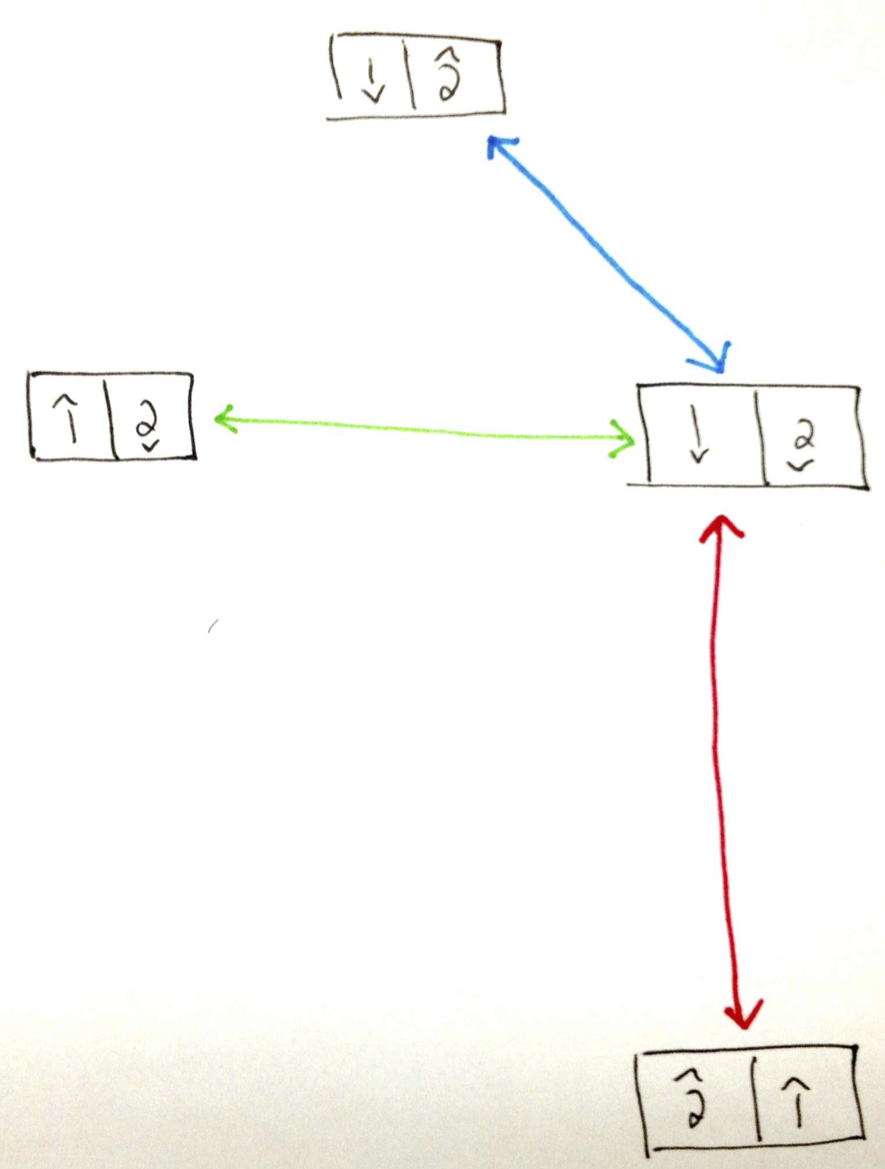
\includegraphics[width=2in]{chunk_cayley_spin1by2.png}
\end{center}

\noindent Notice we have three different colored arrows.  Can you see what each of the colors corresponds to?  If we include the rest of the scrambled boards and all possible spins, we obtain the complete Cayley diagram for $\Spin_{1\times 3}$.  (I'll replace my hand drawn version later.)

\begin{center}
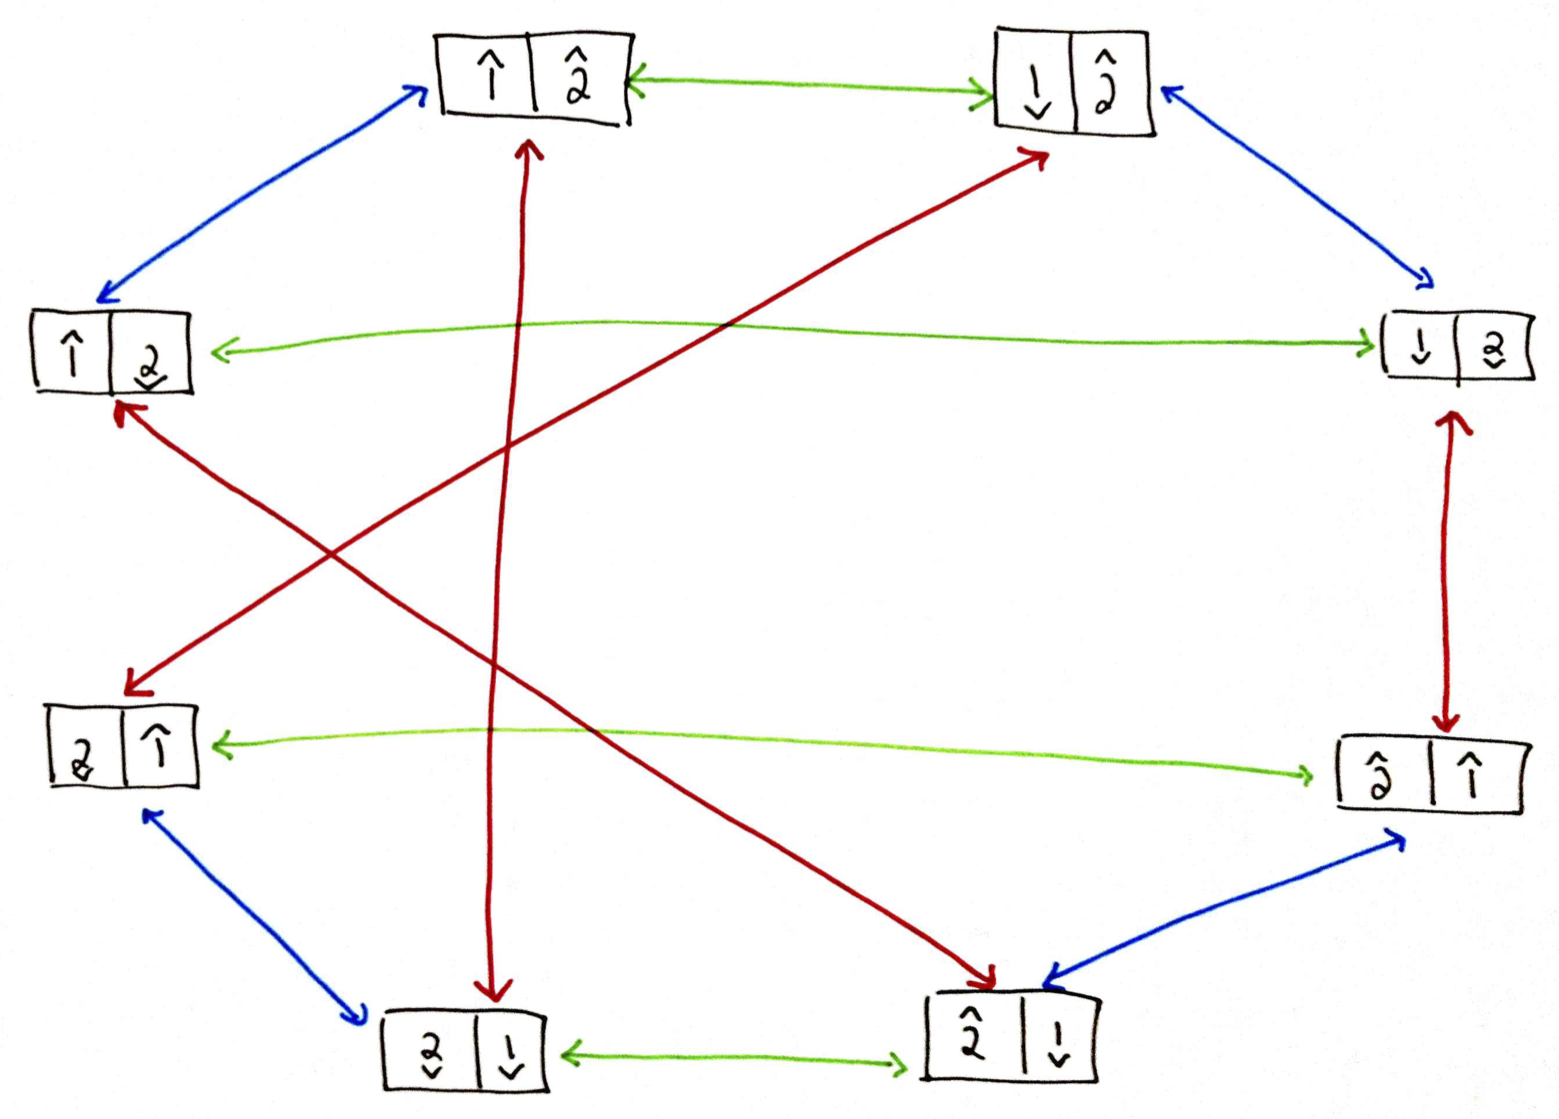
\includegraphics[width=4in]{cayley_spin1by2.png}
\end{center}

\noindent In this case, the spins that correspond to the three arrow colors are the \textbf{generators} of $\Spin_{1\times 2}$.  What this means is that we can obtain all possible scramblings/unscramblings by using just these 3 spins.  In other words, each of the scramblings corresponds to a word in these three spins.  The question remains as to whether we want each board to correspond to a word that unscrambles to the solve board or scrambles the solved board.  This might seem counter to how you want it to be, but we'll adopt the convention that each board corresponds to words that scramble the solved board into the desired scrambled board.

Let $t_1$ be the spin that toggles position 1, $t_2$ be the spin that toggles position 2, and $s_1$ be the spin that rotates the full board.  Recall that when we write down words, we should apply the actions from right to left (like function composition).  

Consider the following scrambled board.

\begin{center}
\begin{tikzpicture}[every node/.style={minimum size=.65cm}]
  \node [draw] (1) {{$\underline{2}$}};
  \node [draw, right=0cm of 1] (2) {\rotatebox{180}{$\underline{1}$}};
\end{tikzpicture}
\end{center}

\noindent Looking at our Cayley diagram for $\Spin_{1\times 2}$, we see that one way to get to this board from the solved board is to follow a blue arrow followed by a red arrow.  This corresponds to the word $s_1t_2$.  However, it also corresponds to the word $t_2s_1t_2t_1$ even though this is not an optimal solution.

\begin{exercise}
Given a word that corresponds to a scrambled board in the Cayley diagram for $\Spin_{1\times 2}$, how could we obtain a solution to the scrambled board?
\end{exercise}

\begin{exercise}
Using the Cayley diagram for $\Spin_{1\times 2}$, find three distinct words that correspond to the following scrambled board.  Don't worry about whether your word is of optimal length or not.

\begin{center}
\begin{tikzpicture}[every node/.style={minimum size=.65cm}]
  \node [draw] (1) {\rotatebox{180}{$\underline{1}$}};
  \node [draw, right=0cm of 1] (2) {\rotatebox{180}{$\underline{2}$}};
\end{tikzpicture}
\end{center}
\end{exercise}

\begin{exercise}
Consider the Cayley diagram for $\Spin_{1\times 2}$, but remove all the red arrows.  This corresponds to forbidding the spin that rotates the full $1\times 2$ board.  Can we obtain all of the scrambled boards from the solved board using only blue and green arrows?
\end{exercise}

\begin{exercise}
Repeat the previous exercise, but this time remove only the green arrows.  What about the blue arrows?
\end{exercise}

In general, a \textbf{Cayley diagram} for a group $G$ is a digraph having the set of actions of $G$ as its vertices and the directed edges (i.e., arrows) correspond to the generators of the group.  Recall that the generators are a potentially smaller set of actions from which you can derive all the actions of the group.  The way you can derive new actions is by forming words in the generators.  Rule 2 guarantees that every action is reversible, so we also allow the use of a generator's reversal in our words.  

The arrows follow the direction of the action that it corresponds to. If a generator is its own reversal, then the arrows corresponding to that generator are two-way arrows.  It is always true that following an arrow backwards corresponds to a generator's reversal.  We need a way to tell our arrow types apart.  One way to do this is to color them.  Another way would be to label the arrows by their corresponding generator.

Remember that in any group there is always a do-nothing action.  One of the vertices should be labeled as the do-nothing action.  From this point forward, unless someone says otherwise, let's use $e$ to denote our do-nothing action for a group.  Each vertex is labeled with a word that corresponds to the sequence of arrows that we can follow from the do-nothing action to the particular vertex.  Since there are possibly many sequences of arrows that could take us from the do-nothing vertex to another, each vertex could be labeled with many different words.

In the Cayley diagram for $\Spin_{1\times 2}$, our vertices were fancy pictures of scrambled $1\times 2$ Spinpossible boards.  This wasn't necessary, but is convenient and appealing for aesthetic reasons.  Also, we never actually labeled the vertices with the corresponding words.  However, these are easy to obtain by following the sequence of arrows.  Of course, in order to do this, we need to know that the vertex that is the solved board corresponds to the do-nothing action.

The next two exercises may be too abstract for you at the moment.  Give them a shot and if you can't do them now, come back to them after you've constructed a few Cayley diagrams.

\begin{exercise}
Assume $G$ is a group and $S$ is a set of generators for $G$. Suppose we draw the Cayley diagram for $G$ using the actions of $S$ as our arrows and we color the arrows according to which generator they correspond to.  Assume that each vertex is labeled with a word.  If the arrows are not labeled, how can you tell which generator they correspond to?
\end{exercise}

\begin{exercise}
Assume $G$ is a group.  Suppose that $S$ and $S'$ are two different sets that generate $G$.  If you draw the Cayley diagram for $G$ using $S$ and then draw the Cayley diagram for $G$ using $S'$, what features of the two graphs are the same and which are potentially different?
\end{exercise}

Let's build a few more Cayley diagrams to further our intuition.

\begin{exercise}
Consider the group consisting of the actions that rearranges two coins, say a penny and a nickel.  Let's assume we start with the penny of the left and the nickel on the right.  Let's call this group $S_2$.

\begin{enumerate}
\item[(a)] Write down all possible actions using verbal descriptions.  \emph{Hint:} There aren't that many of them.
\item[(b)] Let $s$ be the action that swaps the left and right coins.  Does $s$ generate $S_2$?  That is, can we write all of the actions of $S_2$ as words in $s$ (or its reversal)?
\item[(c)] Decide on a simple generating set for $S_2$ and draw a Cayley diagram for $S_2$ using your generating set.  Label all the vertices and arrows appropriately.  Recall that above we said that we will use $e$ to denote the do-nothing action unless someone says otherwise.
\end{enumerate}
\end{exercise}

\begin{exercise}
Consider a square puzzle piece that fits perfectly into a square hole.  Let $R_4$ be the group of actions consisting of rotating the square by an appropriate amount so that it fits back into the hole.
\begin{enumerate}
\item[(a)] Write down all possible actions using verbal descriptions.  Are there lots of ways to describe each of your actions?
\item[(b)] Let $r$ be the action that rotates the puzzle piece by $90^\circ$ clockwise.  Does $r$ generate $R_4$?  If so, write down all of the actions of $R_4$ as words in $r$.
\item[(c)] Which of your words above is the reversal of $r$?
\item[(d)] Draw the Cayley diagram for $R_4$ using $r$ as the generator.  Be sure to label the vertices and arrows.  Are your arrows one-way or two-way arrows?
\end{enumerate}
\end{exercise}

\begin{exercise}
Consider a puzzle piece like the one in the previous exercise, except this time, let's assume that the piece and the hole are an equilateral triangle.  Let $D_3$ be the group of actions that allow the triangle to fit back in the hole.  In addition to rotations, we will also allow the triangle to be flipped over.  To give us a common starting point, let's assume the triangle and hole are positioned so that a base of the triangle is down.  Also, let's label both the points of the hole and the points of the triangle with the numbers 1, 2, and 3.  Assume the labeling on the hole starts with 1 on top and then continues around in the obvious way going clockwise.  Label the puzzle piece in the same way and let's assume that the triangle starts in the position that has the labels matching (i.e., the point of the triangle labeled 1 is in the corner of the hole labeled 1, etc.).
\begin{enumerate}
\item[(a)] How many actions are there?  Can you describe them?  One way to do this would be to indicate where the labels of the triangle are in the hole.
\item[(b)] Let $r$ be rotation by $120^\circ$ in the clockwise direction.  Does $r$ generate $D_3$?
\item[(c)] What is the reversal of $r$?  Can you write it as a word in $r$?
\item[(c)] Let $s$ be the flip (or we could call it a reflection) that swaps the corners of the puzzle piece that are in the positions of the hole labeled by 2 and 3 (this leaves the corner in position 1 of the hole in the same spot).  Does $s$ generate $D_3$?
\item[(d)] What is the reversal of $s$?  Can you write it as a word?
\item[(e)] Can we generate all of $D_3$ using both $r$ and $s$?  If so, write all the actions of $D_3$ as words in $r$ and $s$ (or their reversals).
\item[(f)] Draw the Cayley diagram for $D_3$ using $r$ and $s$ as your arrows.  \emph{Hints:} One of your arrow types is one-way and the other is two-way.  I suggest putting half the vertices in a circle and then the other half in a concentric circle outside your first half.  Label one of the vertices on the inner circle as $e$ and first think about applying consecutive actions of $r$.  Try to stay on the inner circle of vertices as you do this.  Now, starting at $e$, apply $s$ and go to one of the vertices in the outer circle.  Try to label the remaining vertices using both $r$ and $s$.  There are multiple ways to do it.
\end{enumerate}
\end{exercise}

\begin{exercise}
Repeat the above exercise, but do it for a square instead of a triangle.  You'll need to make some modifications to $r$ and $s$.  The resulting group is called $D_4$.
\end{exercise}
\chapter{An Introduction to Subgroups and Isomorphisms}
\label{chapter:intro_subgroups_isomorphisms}
\thispagestyle{empty}

In this chapter, we'll continue to utilize our intuitive definition of a group.  That is, a group $G$ is a set of actions that satisfies the following rules.

\begin{description}
\item[Rule 1.] There is a predefined list of actions that never changes.
\item[Rule 2.] Every action is reversible.
\item[Rule 3.] Every action is deterministic.
\item[Rule 4.] Any sequence of consecutive actions is also an action.
\end{description}

In the previous chapter, we constructed lots of Cayley diagrams for various groups.  To construct a Cayley diagram for a group $G$, we need to first identify a set of generators, say $S$.  Recall that our choice of generators is important as changing the generators can result in a different Cayley diagram.  

In the Cayley diagram for $G$ using $S$, all the actions of $G$ are represented by the vertices of the graph.  Each vertex corresponds to a unique action.  This does not imply that there is a unique way to obtain a given action from the generators.  Each of the generators determines an arrow type in the diagram.  One way to distinguish the different arrow types is by using different colors.  An arrow of a particular color always represents the same generator.

One of the vertices in the diagram is labeled by the do-nothing action, often denoted by $e$.  Each of the other vertices are labeled by words that correspond to following arrows (forwards or backwards) from $e$ to a given vertex.  There may be many ways to do this as each sequence of arrows corresponds to a unique word.  So, a vertex could be potentially labeled by many words.  However, we'll often just pick one.  Also, one potentially confusing item is that we read our words from right to left.  That is, the first arrow we follow out of $e$ is the rightmost generator in the word.

\begin{section}{Subgroups}

\begin{exercise}
Recall the definition of ``subset."  What do you think ``subgroup" means?  Try to come up with a potential definition.  Try not to read any further before doing this.
\end{exercise}

Before continuing, gather up the following Cayley diagrams:
\begin{itemize}
\item $\Spin_{1\times 2}$. There are 3 of these.  I drew one for you in Chapter~\ref{chapter:cayley_diagrams} and you discovered two more in Exercise~\ref{exer:minimal_Cayley_Spin1by2}.
\item $S_2$.  See Exercise~\ref{exer:introducing_S2}.
\item $R_4$.  See Exercise~\ref{exer:introducing_R4}.
\item $D_3$.  There are two of these.  See exercises \ref{exer:introducing_D3} and \ref{exer:alternate_D3}.
\item $D_4$.  See Exercise~\ref{exer:introducing_D4}.
\end{itemize}

\begin{exercise}\label{exer:R4_in_D4}
Examine your Cayley diagrams for $D_4$ and $R_4$.  Make some observations.  How are they similar and how are they different?  Can you reconcile the similarities and differences by thinking about the actions of each group?
\end{exercise}

Hopefully, one of the things you noticed in the previous exercise is that we can ``see" $R_4$ inside of $D_4$ (and hopefully you didn't just read that before completing the exercise).  You may have used different colors in each case and maybe even labeled the vertices with different words, but the overall structure of $R_4$ is there nonetheless.

\begin{exercise}\label{exer:R4_subgroup_D_4}
If you just pay attention to the configuration of arrows, it appears that there are two copies of the Cayley diagram for $R_4$ in the Cayley diagram for $D_4$.  Isolate these two copies by ignoring the edges that correspond to the generator $s$.  Paying close attention to the words that label the vertices from the original Cayley diagram for $D_4$, are either of these groups in their own right?
\end{exercise}

Recall that the do-nothing action must always be one of the actions included in a group.  If this didn't occur to you when doing the previous exercise, you might want to go back and rethink your answer.  Just like in the previous exercise, we can often ``see" smaller groups living inside larger groups.  These smaller groups are called \textbf{subgroups}.

\begin{intuitivedef}
Let $G$ be a group of actions and let $H\subseteq G$.  We say that $H$ is a \textbf{subgroup} if and only if $H$ is a group in its own right.  In this case, we write $H\leq G$.
\end{intuitivedef}

In light of Exercise~\ref{exer:R4_subgroup_D_4}, we would write $R_4\leq D_4$.  The second sub-diagram of $D_4$ that resembles $R_4$ cannot be a subgroup because it does not contain the do-nothing action.  However, since it looks a lot like $R_4$, we call it a \textbf{clone} of $R_4$.

The next theorem\footnote{Perhaps we should call this an ``Intuitive Theorem" since we are using an intuitive definition of a group.} tells us that if we already have a subset of a group, we only need to check two of our rules instead of four.

\begin{theorem}
Let $G$ be a group of actions and let $H\subseteq G$. Then $H$ is a subgroup if and only if $H$ satisfies Rules 2 and 4.%Note: I should probably discuss how the predefined list of generators in Rule 1 is potentially modified.
\end{theorem}

There is one subgroup that every group has.

\begin{theorem}
Let $G$ be a group of actions.  Then $\{e\}\leq G$.
\end{theorem}

\begin{exercise}
Let $G$ be a group and let $e\in G$.  What does the Cayley diagram for the subgroup $\{e\}$ look like?
\end{exercise}

Earlier, we referred to subgroups as being ``smaller."  However, our definition does not imply that this has to be the case.

\begin{theorem}
Let $G$ be a group of actions.  Then $G\leq G$.
\end{theorem}

We refer to subgroups that are strictly smaller than the whole group as \textbf{proper subgroups}.

Lots of groups have been given formal names (e.g., $D_4$, $R_4$, etc.).  However, not every group or subgroup has a name.  In this case, it's useful to have notation to refer to specific subgroups.

\begin{definition}\label{def:subgroup_gen_by}
Let $G$ be a group of actions and let $g_1,\ldots, g_n$ be distinct actions from $G$.  We define $\langle g_1,\ldots, g_n\rangle$ to be the smallest subgroup containing $g_1,\ldots, g_n$.  In this case, we call $\langle g_1,\ldots, g_n\rangle$ the \textbf{subgroup generated by} $g_1,\ldots, g_n$.
\end{definition}

For example, consider $r, s, s'\in D_3$ (as defined in exercises~\ref{exer:introducing_D3} and \ref{exer:alternate_D3}).  Then $\langle r,s\rangle=\langle s, s'\rangle=D_3$.  Recall that $R_4$ was the subgroup of rotations of the square.  Similarly, the group of rotations of an equilateral triangle is called $R_3$.  Then using the $r$ from $D_3$, we have $\langle r\rangle = R_3$, which is a subgroup of $D_3$.

Note that in Definition~\ref{def:subgroup_gen_by}, we used a finite number of generators.  There's no reason we have to do this.  That is, we can consider groups/subgroups generated by infinitely many elements.

\begin{exercise}
Consider $\Spin_{1\times 2}$.  
\begin{enumerate}
\item[(a)] Can you find the Cayley diagram for $\langle t_1\rangle$ as a subgroup of $\Spin_{1\times 2}$?
\item[(b)] Write down all the actions of the subgroup $\langle t_1, t_2\rangle$. Write them as words in $t_1$ and $t_2$.  Can you find the Cayley diagram for $\langle t_1, t_2\rangle$ as a subgroup of $\Spin_{1\times 2}$?  Can you find a clone for $\langle t_1, t_2\rangle$?
\end{enumerate}
\end{exercise}

One of the benefits of Cayley diagrams is that they are usual for visualizing subgroups.  However, recall that if we change our set of generators, we might get a very different looking Cayley diagram.  The upshot of this is that we may be able to see a subgroup in one Cayley diagram for a given group, but not be able to see if Cayley diagram with a different set of arrows.

\begin{exercise}
We currently have two different Cayley diagrams for $D_3$ (see exercises \ref{exer:introducing_D3} and \ref{exer:alternate_D3}).  
\begin{enumerate}
\item[(a)] Can you find the Cayley diagram for $\langle e\rangle$ as a subgroup of $D_3$?  Can you see it in both Cayley diagrams for $D_3$?  Can you find all the clones?
\item[(b)] Can you find the Cayley diagram for $\langle r\rangle =R_3$ as a subgroup of $D_3$?  Can you see it in both Cayley diagrams?  Can you find all the clones?
\item[(c)] Find the Cayley diagrams for $\langle s\rangle$ and $\langle s'\rangle$ as subgroups of $D_3$.  Can you see them in both Cayley diagrams for $D_3$?  Can you find all the clones?
\end{enumerate}
\end{exercise}

\begin{exercise}\label{exer:subgroups_D4}
Consider $D_4$.  Let $h$ be the action that reflects (i.e., flips over) the square over the horizontal midline and let $v$ be the action that reflects the square over the vertical midline.  Also, we'll use $r^2$ as shorthand for the action $rr$ that does $r$ twice in a row.  Which of the following are subgroups of $D_4$?  In each case, justify your answer.  If a subset is a subgroup, try to find a minimal set of generators.  Also, determine whether you can see the subgroups in our Cayley diagram for $D_4$.
\begin{enumerate}
\item[(a)] $\{e, r^2\}$
\item[(b)] $\{e,h\}$
\item[(c)] $\{e, h, v\}$
\item[(d)] $\{e, h, v, r^2\}$
\end{enumerate}
\end{exercise}

The last subgroup above is often referred to as the \textbf{Klein four-group} and is denoted by $V_4$.

Let's introduce a group we haven't seen yet.  We define the \textbf{quaternion group} to be the group $Q_8=\{1,-1,i,-i,j,-j,k,-k\}$ having the following Cayley diagram with generators $i, j, -1$.  In this case, 1 is the do-nothing action.

\tikzstyle{vert} = [circle, draw, fill=grey,inner sep=0pt, minimum size=6mm]
\tikzstyle{b} = [draw,very thick,blue,-stealth]
\tikzstyle{r} = [draw, very thick, red,-stealth]
\tikzstyle{g} = [draw, very thick, green, stealth-stealth]

\begin{center}
\begin{tikzpicture}[scale=1.5,auto]
\node (1) at (135:2) [vert] {{\scriptsize $1$}};
\node (i) at (45:2) [vert] {\scriptsize {$i$}};
\node (k) at (-45:2) [vert] {{\scriptsize $k$}};
\node (j) at (-135:2) [vert] {{\scriptsize $j$}};
\node (-1) at (135:1) [vert] {{\scriptsize $-1$}};
\node (-i) at (45:1) [vert] {{\scriptsize $-i$}};
\node (-k) at (-45:1) [vert] {{\scriptsize $-k$}};
\node (-j) at (-135:1) [vert] {{\scriptsize $-j$}};

\path[b] (1) to (i);
\path[b] (i) to (-1);
\path[b] (-1) to (-i);
\path[b] (-i) to (1);

\path[b] (-j) to (-k);
\path[b] (-k) to (j);
\path[b] (j) to (k);
\path[b] (k) to (-j);

\path[r] (-k) to (-i);
\path[r] (-i) to (k);
\path[r] (k) to (i);
\path[r] (i) to (-k);

\path[r] (1) to (j);
\path[r] (j) to (-1);
\path[r] (-1) to (-j);
\path[r] (-j) to (1);

\path[g] (1) to (-1);
\path[g] (j) to (-j);
\path[g] (i) to (-i);
\path[g] (k) to (-k);

\end{tikzpicture}
\end{center}

Notice that I didn't mention what the actions actually do.  For now, let's not worry about that.  The relationship between the arrows and vertices tells us everything we need to know.  Also, let's take it for granted that $Q_8$ actually is a group.

\begin{exercise}
Consider $Q_8$.
\begin{enumerate}
\item[(a)] Which arrows correspond to which generators in our Cayley diagram for $Q_8$?
\item[(b)] What is $i^2$ equal to?  That is, what element of $\{1,-1,i,-i,j,-j,k,-k\}$ is $i^2$ equal to?  How about $i^3$, $i^4$, and $i^5$?
\item[(c)] What are $j^2$, $j^3$, $j^4$, and $j^5$ equal to?
\item[(d)] What is $(-1)^2$ equal to?
\item[(e)] What is $ij$ equal to?  How about $ji$?
\item[(f)] Can you determine what $k^2$ and $ik$ are equal to?
\item[(g)] Can you identify a generating set consisting of only two elements?  Can you find more than one?
\item[(h)] What subgroups of $Q_8$ can you see in the Cayley diagram (with generators $i, j, -1$)?
\item[(i)] Find a subgroup of $Q_8$ that you cannot see in the Cayley diagram.
\end{enumerate}
\end{exercise}

\end{section}

\begin{section}{Isomorphisms}

By now you've probably seen enough examples of Cayley diagrams to witness some patterns appearing over and over again.  For example, you've seen chunks of Cayley diagrams that resemble the Cayley diagram for $S_2$ with generator $s$.

\tikzstyle{vert} = [circle, draw, fill=grey,inner sep=0pt, minimum size=6mm]
\tikzstyle{twoway} = [draw, very thick, blue, stealth-stealth]

\begin{center}
\begin{tikzpicture}[scale=1.5,auto]
\node (e) at (0,0) [vert] {{\scriptsize $e$}};
\node (s) at (2,0) [vert] {\scriptsize {$s$}};
\path[twoway] (e) to (s);
\end{tikzpicture}
\end{center}

\noindent Recall that $S_2$ is the group that acts on two coins by swapping their positions.  In this case, $s$ is the action that swaps the left and right coins and $e$ is the do-nothing action.  

If you look at any of the versions of the Cayley diagrams for $\Spin_{1\times 2}$, $D_3$, $D_4$, and $Q_8$ that we've seen, it is easy to identify the portions that ``look like" $S_2$.  For example, if you isolate the Cayley diagram for the subgroup $\langle -1\rangle=\{1,-1\}$ in $Q_8$, we see that it looks just like the Cayley diagram for $S_2$, except the labels are not identical.  The clones of the subgroup $\langle -1\rangle=\{1,-1\}$ in $Q_8$ look like $S_2$, as well, but they do not contain the do-nothing action.  

The one thing that is different about the Cayley diagram for $S_2$ and the Cayley diagram for $\langle -1\rangle$ is that the labels are different.  If set the Cayley diagram for $S_2$ on top of the Cayley diagram for $\langle -1\rangle$ such that the do-nothing actions match up, then $s$ and $-1$ would correspond to each other.  In other words, the two Cayley diagrams are identical up to relabeling the vertices.

In this case, we say that $S_2$ and the subgroup $\langle -1\rangle$ of $Q_8$ are \textbf{isomorphic} under the correspondence $e\leftrightarrow 1$ and $s\leftrightarrow -1$.  This one-to-one correspondence between the two groups is called an \textbf{isomorphism}.  

What this means is that these two groups have the same structure and characteristics.  Or, in other words, these two groups essentially do the ``same kind" of thing.  Clearly, the two do-nothing actions behave the same way.  Also, $s$ and $-1$ both have the property that doing the action twice results in having done nothing (i.e., each element is its own reverse).  Since there are only two elements, there isn't anything else to check.  In groups with more elements, things can get much more complicated.  

It is important to point out that $S_2$ and $\langle -1\rangle$ (in $Q_8$) are not equal.  But they have the same structure.  Identifying when to two groups have the same structure (i.e., isomorphic) is an important pursuit in group theory.

If you look at the original Cayley diagram for $\Spin_{1\times 2}$ (with generators $s, t_1, t_2$), we can see three subgroups that look like $S_2$; namely $\langle s\rangle$, $\langle t_1\rangle$, and $\langle t_2\rangle$.  Each of these three subgroups is isomorphic to $S_2$.  

There is one serious potential for confusion here.  Notice that there is an $s$ in $S_2$ and an $s$ in $\Spin_{1\times 2}$.  Despite having identical names, they are not the same element.  Since we only have 26 letters in our alphabet this sort of thing is unavoidable.  Under the isomorphism between $S_2$ and the subgroup $\langle s\rangle$ in $\Spin_{1\times 2}$, the two elements with the same name match up.  That is, these two elements are the ones in each group with the same behavior.

\begin{exercise}
Can you find any other subgroups or groups that are isomorphic to $S_2$?
\end{exercise}

Let's write down an official definition of isomorphic.

\begin{definition}
Let $G$ and $G$ be two groups.  We say that $G_1$ and $G_2$ are \textbf{isomorphic} if there exist generating sets $S$ and $S'$ for $G$ and $G'$, respectively, such that the corresponding Cayley diagrams are identical where we ignore the labels on the vertices and recolor the edges if necessary.  In this case, we write $G\cong G'$.  Otherwise, we say that $G$ and $G'$ are not isomorphic.  If $G$ and $G'$ are isomorphic, then the one-to-one correspondence determined by matching up the corresponding generators and respecting arrow paths is called an \textbf{isomorphism}.
\end{definition}

The last sentence in the definition above might be a bit much to handle at the moment, but as we construct more examples, the concept should become clear.  The general idea is to take to to identical Cayley diagrams (ignoring labels) for $G$ and $G'$ and then set one on top of the other so that the vertices and arrows of the same color match up.  This should be done so that the do-nothing actions correspond to each other.  Then it becomes clear which actions in $G$ correspond to which actions in $G'$.  There might be many ways to do this.

Consider the group $R_4$ with generator $r$ (rotation by $90^\circ$ clockwise).  Now, take a look at the Cayley diagram for $Q_8$ with generators $i, j, -1$.  It should be easy to convince yourself that $R_4$ is isomorphic to both $\langle i\rangle=\{1,i,-i,-1\}$ and $\langle j\rangle=\{1,j,-j,-1\}$.  However, you have to do some rearranging of one of the diagrams to set one on top of the other.  Let's just focus on $\langle i\rangle$.  

How do $R_4$ and $\langle i\rangle$ match up?  We want to pair elements in each group with an element in the other group that has the same behavior.  Clearly, $e$ and $1$ match up since these are the two do-nothing actions.  Also, the reason why we noticed these two groups were isomorphic is because their Cayley diagrams looked the same.  Since each Cayley diagram only had one arrow type determined by $r$ and $i$, we should pair these two elements.  Now, following the arrows around the diagram, we see that $r^2$ must pair with $i^2=-1$ and $r^3$ corresponds to $i^3=-i$.  In summary, the isomorphism between $R_4$ and $\langle i\rangle$ (in $Q_8$) is given by $e\leftrightarrow 1$, $r\leftrightarrow r$, $r^2\leftrightarrow -1$, and $r^3\leftrightarrow -i$.  You should take a moment to convince yourself that the elements that correspond to each other really do behave in similar ways.

Now, take a look at the Cayley diagram for $D_4$ with generators $r$ and $s$.  As we noticed in Exercise~\ref{exer:R4_in_D4}, $R_4$ is a subgroup of $D_4$.  We could say that this subgroup is isomorphic to $R_4$, but in this case, we can say something even stronger: they are equal!

It turns out that there is a fancy word for the size of a group.

\begin{definition}
If $G$ is a group with $n$ distinct actions, then we say that $G$ has \textbf{order} $n$ and write $|G|=n$.  If $G$ contains infinitely many elements, then we say $G$ has infinite order and write $|G|=\infty$.
\end{definition}

\begin{exercise}
Find the orders of the following groups: $S_2$, $\Spin_{1\times 3}$, $\Spin_{3\times 3}$, $R_4$, $D_3$, $D_4$, $V_4$ (see the comment following Exercise~\ref{exer:subgroups_D4}), and $Q_8$.
\end{exercise}

\begin{theorem}
Suppose $G$ and $G'$ are two groups of actions such that $G\cong G'$.  Then $|G|=|G'|$.
\end{theorem}

Unfortunately, the converse of the previous theorem is not true in general.  That is, two groups that have the same order may or may not be isomorphic.  

Loosely speaking, if one group has a property that the other does not have, then the two groups cannot be isomorphic.  For example, if one group has the property that every pair of actions commutes (i.e., the order\footnote{Don't confuse the word ``order" in this sentence with the order of a group.} of the actions does not matter), but another group has a pair of actions that do not commute, then the two groups cannot be isomorphic.  Moreover, if one group contains an action that requires a minimum of $k$ applications to get back to the do-nothing action, but a second group does not have such an element, then the two groups cannot be isomorphic.  

Justifying these two claims takes a bit of work and for now, we'll put that on hold.  For the time being, if you don't see why these claims about when two groups are not isomorphic are true, just take them on faith and we will return to the issue in a later chapter.  Feel free to use these ideas in the exercises that follow.

Let's do a bit more exploring.

\begin{exercise}
Using $h$ and $v$ as generators, draw the Cayley diagram for $V_4$.
\end{exercise}

Notice that our standard Cayley diagram for $R_4$ does not look like the Cayley diagram that you just constructed for $V_4$.  This does \emph{not} imply that these two groups are not isomorphic.

\begin{problem}
Determine whether $R_4$ and $V_4$ are isomorphic.  Justify your answer.  If they are isomorphic, specify the isomorphism by listing the correspondence of elements.
\end{problem}

\begin{problem}
Consider the group given by the Cayley diagram in Exercise~\ref{exer:intro_R6}.  Let's assume that this is the rotation group for a regular hexagon---called $R_6$.  Determine whether $R_6$ and $D_3$ are isomorphic.  Justify your answer.  If they are isomorphic, specify the isomorphism by listing the correspondence of elements.
\end{problem}

\begin{exercise}
Consider two light switches on a wall side by side.  Consider the group of actions that consists of all possible actions that you can do to the two light switches.  For example, one action is toggle the left light switch while leaving the right alone.  Let's call this group $L_2$.
\begin{enumerate}
\item[(a)] How many distinct actions does $L_2$ have?
\item[(b)] Can you find a minimal generating set for $L_2$?  If so, give these actions names and then write all of the actions of $L_2$ as words in your generator(s).
\item[(c)] Using your generators from part (b), draw a Cayley diagram for $L_2$.
\end{enumerate}
\end{exercise}

\begin{problem}
Determine whether $L_2$ and $V_4$ are isomorphic.  Justify your answer.  If they are isomorphic, specify the isomorphism by listing the correspondence of elements.
\end{problem}

\begin{problem}
Determine whether $Q_8$ and $D_4$ are isomorphic.  Justify your answer.  If they are isomorphic, specify the isomorphism by listing the correspondence of elements.
\end{problem}

\begin{problem}
Determine whether $\Spin_{1\times 2}$ and $D_4$ are isomorphic.  Justify your answer.  If they are isomorphic, specify the isomorphism by listing the correspondence of elements.
\end{problem}

\begin{exercise}
Consider the group that acts on three coins that are in a row by rearranging their positions (but not flipping them over).  This group is called $S_3$.  Numbering the positions of the coins (not the coins themselves) 1, 2, 3 from left to right.  Let $s_1$ be the action that swap the coins in positions 1 and 2.  Similarly, let $s_2$ be the action that swaps coins in positions 2 and 3.
\begin{enumerate}
\item[(a)] The group $S_3$ consists of 6 actions, which we can generate with $s_1$ and $s_2$.  Write all 6 actions as words in $s_1$ and $s_2$.
\item[(b)] Using $s_1$ and $s_2$ as generators, draw a Cayley diagram for $S_3$.
\end{enumerate}
\end{exercise}

\begin{problem}
Determine whether $S_3$ and $D_3$ are isomorphic.  Justify your answer.  If they are isomorphic, specify the isomorphism by listing the correspondence of elements.  Don't forget that we've drawn two different Cayley diagrams for $D_3$.
\end{problem}

\end{section}
\chapter{A Formal Approach to Groups}
\label{chapter:formal_groups}
\thispagestyle{empty}

In this chapter we finally introduce the formal definition of a group.  From this point on, our focus will shift from developing intuition to studying the abstract properties of groups.  However, we should not abandon the intuition we have gained.  As we progress, your intuitive understanding of groups will continue to improve and you should rely on this understanding as you try to make sense of the notions that follow.  There has been plenty of intentional foreshadowing, so expect to revisit concepts you've already encountered.  We'll also encounter plenty of new stuff, too.

It is important to point out that things are about to get quite a bit more difficult for most of you.  Be patient and persistent!

\begin{section}{Binary Operations}
After learning to count as a child, you likely learned how to add, subtract, multiply, and divide with natural numbers.  Loosely speaking, these operations are examples of binary operations since we are combining two objects to obtain a single object.  More formally, we have the following definition.

\begin{definition}
A \textbf{binary operation} $*$ on a set $A$ is a function from $A\times A$ into $A$.  For each $(a,b)\in A\times A$, we denote the element $*(a,b)$ via $a*b$.
\end{definition}

\begin{remark}
Don't misunderstand the use of $*$ in this context.  We are not implying that $*$ is the ordinary multiplication of real numbers that you are familiar with.  We use $*$ to represent a generic binary operation.  
\end{remark}

\begin{remark}
Notice that since the codomain of a binary operation on a set $A$ is $A$, binary operations require that we yield an element of $A$ when combining two elements of $A$.  In this case, we say that $A$ is \textbf{closed} under $*$.  Binary operations have this closure property by definition.  Also, since binary operations are functions, any attempt to combine two elements from $A$ should result in a \emph{unique} element of $A$.  In this case, we say that $*$ is \textbf{well-defined}.  Moreover, since the domain of $*$ is $A\times A$, it must be the case that $*$ is defined for \emph{all} pairs of elements from $A$.
\end{remark}

\begin{example}
Examples of binary operations include $+$ (addition), $-$ (subtraction), and $\cdot$ (multiplication) on the real numbers.  However, $\div$ (division) is not a binary operation on the set of real numbers because all elements of the form $(a,0)$ are not in the domain $\mathbb{R}\times \mathbb{R}$ since we cannot divide by 0.  Yet, $\div$ is a suitable binary operation on $\mathbb{R}\setminus \{0\}$.
\end{example}

\begin{example}
Let $C$ be the set of continuous functions from $\mathbb{R}$ to $\mathbb{R}$.  Then $\circ$ (function composition) is a binary operation on $C$.
\end{example}

\begin{example}
Consider the 6 actions of $D_3$.  The composition of these actions is a binary operation on $D_3$.  In fact, composition of actions for each of the groups that we have seen is a binary operation on the given group.  Notice that we never used a symbol for these binary operations, but rather used juxtaposition (i.e., $ab$ is the juxtaposition of $a$ and $b$).
\end{example}

\begin{example}
Let $M_{2\times 2}(\mathbb{R})$ be the set of $2\times 2$ matrices with real number entries.  Then matrix multiplication is a binary operation on $M_{2\times 2}(\mathbb{R})$.
\end{example}

\begin{exercise}
Explain why composition of spins is not a binary operation on the set of allowable spins in $\Spin_{3\times 3}$.
\end{exercise}

\begin{exercise}
Let $M(\mathbb{R})$ be the set of matrices (of any size) with real number entries.  Is matrix addition a binary operation on $M(\mathbb{R})$?  How about matrix multiplication?
\end{exercise}

\begin{exercise}
Determine whether $\cup$ (union) and $\cap$ (intersection) are binary operations on $\mathcal{P}(\mathbb{Z})$ (i.e., the power set of the integers).
\end{exercise}

\begin{exercise}
Consider the closed interval $[0,1]$ and define $*$ on $[0,1]$ via $a*b=\mathrm{min}\{a,b\}$ (i.e., take the minimum of $a$ and $b$).  Determine whether $*$ is a binary operation on $[0,1]$.
\end{exercise}

Some binary operations have additional properties.

\begin{definition}
Let $A$ be a set and let $*$ be a binary operation on $A$.
\begin{enumerate}
\item We say that $*$ is \textbf{associative} if and only if $(a*b)*c=a*(b*c)$ for all $a,b,c\in A$.
\item We say that $*$ is \textbf{commutative} if and only if $a*b=b*a$ for all $a,b\in A$.
\end{enumerate}
\end{definition}

\begin{exercise}
Provide at least one example of a binary operation and the corresponding set that is commutative.  How about not commutative?
\end{exercise}

\begin{theorem}
Let $A$ be a set and let $F$ be the set of functions from $A$ to $A$.  Then function composition is an associative binary operation on $F$.
\end{theorem}

When the set $A$ is finite, we can represent a binary operation on $A$ using a table in which the elements of the set are listed across the top and the left side (in the same order).  The entry in the $i$th row and $j$th column of the table represents the output of combining the element that labels the $i$th row with the element that labels the $j$th column (order matters).

\begin{example}\label{example:table}
Consider the following table.
\begin{center}
\begin{tabu}{c|[2pt]c|c|c}
$*$ & $a$ & $b$ & $c$ \\ \tabucline[2pt]{-}
$a$ & $b$ & $c$ & $b$ \\
\hline $b$ & $a$ & $c$ & $b$  \\
\hline $c$ & $c$ & $b$ & $a$
\end{tabu}
\end{center}
This table represents a binary operation on the set $A=\{a,b,c\}$.  In this case, $a*b=c$ while $b*a=a$.  This shows that $*$ is not commutative.
\end{example}

\begin{exercise}
What property must a table for a binary operation have in order for the operation to be commutative?
\end{exercise}

\begin{exercise}\label{exer:table_missing_entries}%Exercise 1.2.6 in Fraleigh
Fill in the missing entries in the following table so that $*$ defines an associative binary operation on $\{a,b,c,d\}$.
\begin{center}
\begin{tabu}{c|[2pt]c|c|c|c}
    $*$ & $a$ & $b$ & $c$ & $d$ \\\tabucline[2pt]{-}
    $a$ & $a$ & $b$ & $c$ & $d$ \\\hline
    $b$ & $b$ & $a$ & $c$ & $d$ \\\hline
    $c$ & $c$ & $d$ & $c$ & $d$ \\\hline
    $d$ &  &  & & 
\end{tabu}
\end{center}
\end{exercise}

\end{section}

\begin{section}{Groups}
Without further ado, here is our official definition of a group.

\begin{definition}\label{def:group}
A group $(G,*)$ is a set $G$ together with a binary operation $*$ such that the following axioms hold.
\begin{enumerate}
\item[0.] The set $G$ is closed under $*$.
\item[1.] The operation $*$ is associative.
\item[2.] There is an element $e\in G$ such that for all $g\in G$, $e*g=g*e=g$.  We call $e$ the \textbf{identity}.
\item[3.] Corresponding to each $g\in G$, there is an element $g'\in G$ such that $g*g'=g'*g=e$.  In this case, $g'$ is called the \textbf{inverse} of $g$, which we shall denote as $g^{-1}$.
\end{enumerate}
\end{definition}

\begin{remark}
A few comments are in order.
\begin{enumerate}
\item Notice that a group has two parts to it, namely, a set and a binary operation.  For simplicity, if $(G,*)$ is a group, we will often refer to $G$ as being the group.  However, you must remember that the binary operation is part of the structure.
\item Axiom 2 forces $G$ to be nonempty.
\item In the generic case, even if $*$ is not actually multiplication, we will refer to $a*b$ as the \textbf{product} of $a$ and $b$.
\item We are not requiring $*$ to be commutative.  If $*$ is commutative, then we say that $G$ is \textbf{abelian}\footnote{Commutative groups are called abelian in honor of the Norwegian mathematician Niels Abel (1802--1829).} (or \textbf{commutative}).
\end{enumerate}
\end{remark}

\begin{exercise}
Explain why Axiom 0 is unnecessary.
\end{exercise}

At this time, we have two definitions of a group.  The first one was intended to provide an intuitive introduction and Definition~\ref{def:group} provides a rigorous mathematical definition.  We should confirm that these two definitions are in fact compatible.

\begin{exercise}
Compare and contrast our two definitions of a group.  How do the rules and axioms match up?
\end{exercise}

\begin{exercise}
Quickly verify that $\Spin_{1\times 2}$, $S_2$, $R_4$, $D_3$, $D_4$, $V_4$, and $Q_8$ are groups under composition of actions.
\end{exercise}

\begin{exercise}
Determine whether each of the following are groups.  If the pair is a group, determine whether it is abelian and identify the identity.  Explain your answers.
\begin{enumerate}[label=\rm{(\alph*)}]
\item $(\mathbb{Z},+)$
\item $(\mathbb{N},+)$
\item $(\mathbb{Z},\cdot)$
\item $(\mathbb{R},+)$
\item $(\mathbb{R},\cdot)$
\item $(\mathbb{R}\setminus \{0\},\cdot)$
\item $(M_{2\times 2}(\mathbb{R}),+)$
\item $(M_{2\times 2}(\mathbb{R}),*)$, where $*$ is matrix multiplication.
\item $(\{a,b,c\},*)$, where $*$ is the operation determined by the table in Example~\ref{example:table}.
\item $(\{a,b,c,d\},*)$, where $*$ is the operation determined by the table in Exercise~\ref{exer:table_missing_entries}.
\end{enumerate}
\end{exercise}

Notice that in Axiom 2 of Definition~\ref{def:group}, we said \emph{the} identity and not \emph{an} identity.  Implicitly, this implies that the identity is unique.

\begin{theorem}\label{thm:unique_id}
Let $G$ be a group with binary operation $*$.  Then there is a unique identity element in $G$.  That is, there is only one element $e$ in $G$ such that $g*e=e*g=g$ for all $g\in G$.
\end{theorem}

The following theorem is crucial for proving many theorems about groups.

\begin{theorem}[Cancellation Law]
Let $(G,*)$ be a group and let $g,x,y\in G$.  Then $g*x=g*y$ if and only if $x=y$.  Similarly, $x*g=y*g$ if and only if $x=y$.\footnote{You only need to prove one of these statements as the proof of the other is symmetric.}
\end{theorem}

\begin{exercise}
Show that $(\mathbb{R},\cdot)$ fails the Cancellation Law (confirming the fact that it is not a group).
\end{exercise}

\begin{corollary}
Let $G$ be a group with binary operation $*$.  Then each $g\in G$ has a unique inverse.
\end{corollary}

\begin{theorem}\label{thm:unique_soln}
Let $(G,*)$ be a group and let $g,h\in G$.  Then the equations $g*x=h$ and $y*g=h$ have unique solutions for $x$ and $y$ in $G$.  
\end{theorem}

While proving the previous few theorems, hopefully one of the things you realized is that you can multiply both sides of a group equation by the same element but that you have to do it on the same side of each half.  That is, since a group may or may not be abelian, if I multiply one side of an equation on the left by a group element, then we must multiply the other side of the equation on the left by the same group element.

Despite the fact that a group may or may not be abelian, if one product is equal to the identity, then reversing the order yields the same result.

\begin{theorem}
Let $G$ be a group with binary operation $*$.  If $g*h=e$, then $h*g=e$.
\end{theorem}

The upshot of the previous theorem is if we have a ``left inverse" then we automatically have a ``right inverse" (and vice versa).

The next theorem should not be surprising.

\begin{theorem}
Let $(G,*)$ be a group and let $g\in G$.  Then $(g^{-1})^{-1}=g$.
\end{theorem}

\begin{definition}
Let $(G,*)$ be a group and let $g\in G$.  Then for $n\in \mathbb{N}$, we define
\[
g^n=\underbrace{g*g*\cdots *g}_{n\text{ factors}}
\]
and
\[
g^{-n}=\underbrace{g^{-1}*g^{-1}*\cdots *g^{-1}}_{n\text{ factors}}.
\]
Moreover, we define $g^0=e$.
\end{definition}

The good news is that the rules of exponents you are familiar with still hold for groups.

\begin{theorem}
Let $(G,*)$ be a group and let $g\in G$.  If $n\in\mathbb{Z}$, then:
\begin{enumerate}
\item $g^n*g^m=g^{n+m}$,
\item $(g^n)^{-1}=g^{-n}$.
\end{enumerate}
\end{theorem}

\end{section}

\begin{section}{Group Tables}
Recall that we could represent a binary operation on a finite set using a table.  Since groups have binary operations at their core, we can represent a finite group (i.e., a group with finitely many elements) using a table, called a \textbf{group table} (or \textbf{Cayley table}). For example, the following is a group table for $V_4$.

\begin{center}
\begin{tabu}{c|[2pt]c|c|c|c}
$*$ & $e$ & $v$ & $h$ & $vh$ \\ \tabucline[2pt]{-}
$e$ & $e$ & $v$ & $h$ & $vh$ \\
\hline $v$ & $v$ & $e$ & $vh$ & $h$  \\
\hline $h$ & $h$ & $vh$ & $e$ & $v$\\
\hline $vh$ & $vh$ & $h$ & $v$ & $e$
\end{tabu}
\end{center}

\begin{exercise}
Verify that $V_4$ is an abelian group.  What feature of the group table makes this clear?
\end{exercise}

Notice that above I said, ``a group table for $V_4$" and not ``the group table."  The reason for this is that if we chose a different order of the elements (e.g., swap rows 1 and 4---which swaps columns 1 and 4, as well), then the table would look slightly different.  Also, if we had chosen a different generating set, then the names of the elements would look different.  Regardless, the table still captures the same information about the binary operation.

\begin{exercise}
Create group tables for the following groups: $S_2$, $R_3$, $R_4$, $D_3$, $S_3$, $D_4$, and $Q_8$.  Which groups are abelian?
\end{exercise}

Perhaps you noticed when creating the tables above that each element of the group appeared exactly once in each row and column, respectively.  This is true, in general.  Use Theorem~\ref{thm:unique_soln}, to prove the following theorem.

\begin{theorem}
Let $(G,*)$ be a finite group.  Then each element of $G$ appears exactly once in each row and each column, respectively, in any group table for $G$.
\end{theorem}

We can also use tables to define groups.  For example, consider the following table on the set $A=\{e,a,b,c\}$.

\begin{center}
\begin{tabu}{c|[2pt]c|c|c|c}
$*$ & $e$ & $a$ & $b$ & $c$ \\ \tabucline[2pt]{-}
$e$ & $e$ & $a$ & $b$ & $c$ \\
\hline $a$ & $a$ & $e$ & $c$ & $b$  \\
\hline $b$ & $b$ & $c$ & $e$ & $a$\\
\hline $c$ & $c$ & $b$ & $a$ & $e$
\end{tabu}
\end{center}

\noindent Is this a table for a group?  First, we see that the binary operation determined by the table is closed.  Second, we see that $e$ is acting as the identity.  Since every row and column has the identity element $e$ appearing, we know that every element has an inverse (do you see why that follows?).  The only thing left to check is associativity.  Imagine for a moment what this entails.  It's messy right?!  And this is only for a group of order 4.

Thankfully, we can rely on some prior knowledge to help out with associativity.  It turns out that if you look closely, the group table for $V_4$ looks the ``same" as the table above.  What do we mean by ``same" here?  The names for elements are different (except for $e$), but 
\begin{quotation}
\emph{the product of corresponding elements yields the corresponding result.}
\end{quotation}
To see what I mean, let's color both tables with white, red, blue, and green in such a way that each element corresponds to a unique color.  If we choose our colors wisely, it is easy to see that both tables have the same structure.

\begin{center}
\begin{tabu}{c|[2pt]c|c|c|c}
$*$ & $e$ & \cellcolor{red}$v$ & \cellcolor{blue}$h$ & \cellcolor{green}$vh$ \\ \tabucline[2pt]{-}
$e$ & $e$ & \cellcolor{red}$v$ & \cellcolor{blue}$h$ & \cellcolor{green}$vh$ \\
\hline \cellcolor{red}$v$ & \cellcolor{red}$v$ & $e$ & \cellcolor{green}$vh$ & \cellcolor{blue}$h$  \\
\hline \cellcolor{blue}$h$ & \cellcolor{blue}$h$ & \cellcolor{green}$vh$ & $e$ & \cellcolor{red}$v$\\
\hline \cellcolor{green}$vh$ & \cellcolor{green}$vh$ & \cellcolor{blue}$h$ & \cellcolor{red}$v$ & $e$
\end{tabu}
\hspace{1cm}
\begin{tabu}{c|[2pt]c|c|c|c}
$*$ & $e$ & \cellcolor{red}$a$ & \cellcolor{blue}$b$ & \cellcolor{green}$c$ \\ \tabucline[2pt]{-}
$e$ & $e$ & \cellcolor{red}$a$ & \cellcolor{blue}$b$ & \cellcolor{green}$c$ \\
\hline \cellcolor{red}$a$ & \cellcolor{red}$a$ & $e$ & \cellcolor{green}$c$ & \cellcolor{blue}$b$  \\
\hline \cellcolor{blue}$b$ & \cellcolor{blue}$b$ & \cellcolor{green}$c$ & $e$ & \cellcolor{red}$a$\\
\hline \cellcolor{green}$c$ & \cellcolor{green}$c$ & \cellcolor{blue}$b$ & \cellcolor{red}$a$ & $e$
\end{tabu}
\end{center}

\noindent Since we already know that $V_4$ is a group, we know that the binary operation for $V_4$ is associative.  

\begin{exercise}
Explain why the discussion above implies that the binary operation determined by the table on the right above must be associative.  Have we shown that $(A,*)$ is a group?
\end{exercise}

It is important to point out that if we had not chosen our colors wisely, then perhaps the colorings of the two tables would not agree.  Moreover, if we had made the same color choices for elements, but then rearranged columns and rows of one table, the colorings of the two tables would not agree.  This doesn't imply anything.  The point is whether we \emph{can} get the tables to match.

\begin{exercise}
Draw the Cayley diagram for $(A,*)$ with generators $a$ and $b$.  Explain why this implies that $V_4$ and $A$ (under their respective binary operations) are isomorphic.  
\end{exercise}

\begin{exercise}
Is it possible to color the group table for $R_4$ so that it matches the coloring of $V_4$?  Explain your answer.
\end{exercise}

\begin{problem}\label{prob:iso_same_group_table}
Let $(G,*)$ and $(G',\circ)$ be two finite groups.  Suppose we can arrange the rows and columns and color elements in such a way that the colorings for the two group tables agree.  Explain why this implies that the two groups are isomorphic.
\end{problem}

\begin{problem}
Suppose we have a table for $(G,*)$, where $G$ is finite.  Further suppose that (i) there is an identity element, and (ii) every element appears exactly once in each row and column, respectively.  Explain why the only thing we need to verify in order for $(G,*)$ to be a group is that $*$ is associative.
\end{problem}

\begin{problem}%Exercise 4.18 in VGT
Suppose that $(G,*)$ is a group.  Theorem~\ref{thm:unique_id} guarantees that there is a unique identity in $G$.  When creating the group table for $G$, what goes wrong if you try to include two different identity elements?
\end{problem}

Consider the class of all possible groups.  It turns out that ``isomorphic" ($\cong$) determines an equivalence relation.  That is, under this relation two groups are related if and only if they are isomorphic.  We'll prove this formally later when we have a more rigorous definition of isomorphic.

\begin{problem}
Explain why all groups with a single element are isomorphic.
\end{problem}

In this case, we say that ``up to isomorphism" there is only one group with a single element.

\begin{problem}
Consider a group $(G,*)$ of order 2.  Suppose that $G=\{e,a\}$.  Complete the following group table for $G$.

\begin{center}
\begin{tabu}{c|[2pt]c|c}
$*$ & $e$ & $a$ \\ \tabucline[2pt]{-}
$e$ &  &  \\
\hline $a$ &  & 
\end{tabu}
\end{center}
Explain why every group with 2 elements must be isomorphic to $S_2$.
\end{problem}

The previous problem implies that up to isomorphism, there is only one group of order 2.

\begin{problem}
Consider a group $(G,*)$ of order 3.  Suppose that $G=\{e,a,b\}$.  Complete the following group table for $G$.

\begin{center}
\begin{tabu}{c|[2pt]c|c|c}
$*$ & $e$ & $a$ & $b$ \\ \tabucline[2pt]{-}
$e$ &  &  & \\
\hline $a$ &  & & \\
\hline $b$ &  & &
\end{tabu}
\end{center}
Explain why every group with 3 elements must be isomorphic to $R_3$.
\end{problem}

\begin{problem}
Consider a group $(G,*)$ of order 4.  Suppose that $G=\{e,a,b,c\}$.  Assuming that $e$ is the identity, the first row and first column of the corresponding group table must be completed as follows.

\begin{center}
\begin{tabu}{c|[2pt]c|c|c|c}
$*$ & $e$ & $a$ & $b$ & $c$ \\ \tabucline[2pt]{-}
$e$ &  $e$ & $a$ & $b$ & $c$ \\
\hline $a$ & $a$ & ? & & \\
\hline $b$ & $b$ & & & \\
\hline $c$ & $c$ & & &
\end{tabu}
\end{center}

\noindent The cell with the question mark cannot be filled with an $a$.  So, this entry must be either $e$, $b$, or $c$.  However, it should be easy to see the cases with $b$ and $c$ are symmetric.  Thus, there are two cases: (i) the entry with the question mark is filled with $e$, (ii) the entry with the question mark is (without loss of generality) filled with $b$.  Complete the group table in each of these two cases.  Recall that we've seen two non-isomorphic groups of order 2, namely $R_4$ and $V_4$.  What conclusion can you make about groups of order 4?
\end{problem}

So far we've seen that there are unique groups up to isomorphism of orders 1, 2, and 3, but that there are two groups up to isomorphism of order 4.  A general question we will want to address is, how many groups are there of order $n$?

In a future chapter we will be able to prove that there is only one group up to isomorphism of order 5, namely those groups isomorphic to $R_5$ (i.e., rotation group of a regular pentagon).

We've seen three groups of order 6, namely $R_6$, $D_3$, and $S_3$.  However, $D_3\cong S_3$ (see Problem \ref{prob:D3_iso_S3}) while $R_6$ is not isomorphic to either of these (see Problem \ref{prob:R6_not_iso_D3}).  So, we can conclude that there are at least two groups up to isomorphism of order 6.   But are there others?  It turns out that the answer is yes, but why?

The group $R_7$ is the group of rotations of a regular 7-sided polygon.  This group has order 7.  Are there other groups of order 7 that are not isomorphic to $R_7$? 

We've encountered four groups of order 8, namely $D_4$, $\Spin_{1\times 2}$, $Q_8$, and $R_8$.  Of these, only $D_4$ and $\Spin_{1\times 2}$ are isomorphic.  Thus, there are at least three groups up to isomorphism of order 8.  However, are these the only ones?  It turns out that the answer is no.  What are the missing ones?

\end{section}

\begin{section}{Revisiting Cayley Diagrams and Our Original Definition of a Group}%This section closely mimics Section 6.1 in VGT

Let's begin with a couple exercises.

\begin{exercise}\label{exer:nonRegular1}%Exercise 4.16 in VGT
Consider the diagram given in Figure~\ref{fig:nonRegularRepeat}.  This is identical to the diagram that appeared in Figure~\ref{fig:nonRegular} that we saw at the end of Chapter~\ref{chapter:cayley_diagrams}.
\begin{enumerate}[label=\rm{(\alph*)}]
\item Consider Rules 1--4 of our original definition of a group (see Definition~\ref{def:informal_group}).  Does the diagram in Figure~\ref{fig:nonRegularRepeat} satisfy Rules 1--4?
\item Try to convert this diagram into a group table.  Does the table represent a group? What goes wrong?
\end{enumerate}
\end{exercise}

\begin{figure}[!ht]
\centering
\begin{tikzpicture}[scale=1.5,auto]
\node (a) at (0,0) [vert] {{\scriptsize $a$}};
\node (b) at (2,0) [vert] {{\scriptsize $b$}};
\node (c) at (4,0) [vert] {{\scriptsize $c$}};
\node (d) at (6,0) [vert] {{\scriptsize $d$}};
\node (e) at (6,2) [vert] {{\scriptsize $e$}};
\node (f) at (4,2) [vert] {{\scriptsize $f$}};
\node (g) at (2,2) [vert] {{\scriptsize $g$}};
\node (h) at (0,2) [vert] {{\scriptsize $h$}};

\path[b2] (a) to (b);
\path[b2] (c) to (d);
\path[b2] (h) to (g);
\path[b2] (f) to (e);

\path[r] (b) to (c);
\path[r] (c) to (f);
\path[r] (f) to (g);
\path[r] (g) to (b);

\path[r2] (a) to (h);
\path[r2] (d) to (e);
\end{tikzpicture}
\caption{Diagram for Exercise~\ref{exer:nonRegular1}.}
\label{fig:nonRegularRepeat}
\end{figure}

\begin{exercise}\label{exer:nonRegular2}%Exercise 4.16 in VGT
Consider the diagram given
\begin{enumerate}[label=\rm{(\alph*)}]
\item Does the diagram in Figure~\ref{fig:nonRegular2} satisfy Rules 1--4 of Definition~\ref{def:informal_group}?
\item Try to convert this diagram into a group table.  Does the table represent a group? What goes wrong?
\end{enumerate}
\end{exercise}

\begin{figure}
\centering
\begin{tikzpicture}[scale=1.5,auto]
\node (1) at (0,0) [vert] {};
\node (2) at (2,0) [vert] {};
\node (3) at (4,0) [vert] {};
\node (4) at (6,0) [vert] {};
\node (5) at (0,2) [vert] {};
\node (6) at (2,2) [vert] {};
\node (7) at (4,2) [vert] {};
\node (8) at (6,2) [vert] {};

\path[b] (1) to (5);
\path[b] (2) to (6);
\path[b] (3) to (8);
\path[b] (4) to (7);

\path[r] (1) to (2);
\path[r] (2) to (3);
\path[r] (3) to (4);
\path[r] (4) to [bend left] (1);
\path[r] (5) to (6);
\path[r] (6) to (7);
\path[r] (7) to (8);
\path[r] (8) to [bend right] (5);
\end{tikzpicture}
\caption{Diagram for Exercise~\ref{exer:nonRegular2}.}\label{fig:nonRegular2}
\end{figure}

As the previous two exercises indicate, the moral of the story is that our original intuitive definition of a group has a weakness.  It does not agree with our formal definition of a group given in Definition~\ref{def:group}.  Let's see if we can figure out what goes wrong.

Consider the Cayley diagram for $D_3$ with generating set $\{r,s\}$ that is given in Figure~\ref{fig:D3}. Notice that we labeled the lower right corner of the Cayley diagram with the word $r^2s$.  This means that we first followed a blue arrow out of $e$ and then two red arrows.  However, we could also get to this vertex by first doing a red arrow out of $e$ followed by a blue arrow.  So, we could also have labeled this vertex with the word $sr$.  The upshot is that $r^2s=sr$.  These types of group equations are called \textbf{relations}.

\tikzstyle{vert} = [circle, draw, fill=grey,inner sep=0pt, minimum size=7mm]
\tikzstyle{h} = [draw,very  thick, blue,stealth-stealth]

\begin{figure}
\centering
\begin{tikzpicture}[scale=.75,auto]
\node (e) at (90:2) [vert] {$e$};
\node (r) at (-30:2) [vert] {$r$};
\node (rr) at (210:2) [vert] {$r^2$};
\node (h) at (90:4) [vert] {$s$};
\node (hr) at (210:4) [vert] {$rs$};
\node (hrr) at (-30:4) [vert] {$sr$};
\draw [r] (e) to [bend left] (r);
\draw [r] (r) to [bend left] (rr);
\draw [r] (rr) to [bend left] (e);
\draw [r] (h) to [bend right] (hr);
\draw [r] (hr) to [bend right] (hrr);
\draw [r] (hrr) to [bend right] (h);
\draw [h] (e) to (h);
\draw [h] (r) to (hrr);
\draw [h] (rr) to (hr);
\end{tikzpicture}
\caption{Cayley diagram for $D_3$ with generating set $\{r,s\}$.}\label{fig:D3}
\end{figure}

We discovered this relation by starting at $e$ and then traveling a sequence of arrows to get to the vertex in the lower right corner.  However, notice that following a blue and then two red arrows is \emph{always} the same as following a red arrow and then a blue arrow regardless of which vertex we start at.  That is, the relation $r^2s=sr$ holds universally across the entire Cayley diagram.

Cayley diagrams for groups will always have this uniform symmetry.  The fancy way of saying this is that Cayley diagrams are \textbf{regular}.  In other words, a diagram is regular if every internal pattern repeats itself throughout the diagram.

\begin{exercise}
Identify two other relations that the above Cayley diagram for $D_3$ exhibits.  Find one that involves both $r^{-1}$ (i.e., following a red arrow backwards) and $s$.  Convince yourself that your relations appear throughout the diagram.
\end{exercise}

\begin{exercise}
Verify that the diagrams in Exercise~\ref{exer:nonRegular1} and \ref{exer:nonRegular2} are not regular.
\end{exercise}

\begin{problem}
Explain why the Cayley diagram for a group must be regular.
\end{problem}

The discussion and exercises above lead us to conclude that one thing missing from our original intuitive definition of a group is regularity.  It turns out that this is the only thing missing.  That is, if we add the requirement of regularity to our intuitive definition, we could convert it into a rigorous definition that is equivalent to Definition~\ref{def:group}.  However, we won't bother doing this since our intuitive definition served its purpose.

\end{section}

\begin{section}{Revisiting Subgroups}

Back in Section~\ref{sec:intuitive_subgroups}, we introduced the notion of subgroup.  In light of our official definition of a group, we more or less have the same definition as before, but let's restate it here using slightly more formal language.

\begin{definition}
Let $(G,*)$ be a group and let $H$ be a subset of $G$.  Then $H$ is a \textbf{subgroup} of $G$, written $H\leq G$, provided that $H$ is a group in its own right under the binary operation inherited from $G$.
\end{definition}

The phrase ``under the binary operation inherited from $G$" means that to combine two elements in $H$, we should treat the elements as if they were in $G$ and perform $G$'s binary operation.

Recall that Theorems~\ref{thm:trivial_subgroup1} and \ref{thm:trivial_subgroup2} tell us that $\langle e\rangle=\{e\}$ and $G$ are always subgroups of $G$. This is still true even using our official definition of a group.  These two subgroups are referred to as the \textbf{trivial subgroups}\footnote{Some textbooks will refer to $\{e\}$ as being the trivial subgroup and $G$ as the improper subgroup.}.  All other subgroups are called \textbf{nontrivial}.  If $H$ is a nontrivial subgroup of a group $G$, then we may write $H<G$.

The next theorem tells us that we don't need to verify all the axioms of a group to determine whether a nonempty subset is a subgroup.

\begin{theorem}\label{thm:subgroup_criterion}
Suppose $(G,*)$ is a group and $H$ is a nonempty subset of $G$.  Then $H\leq G$ if and only if (i) for all $h\in H$, $h^{-1} \in H$, as well, and (ii) $H$ is closed under the binary operation of $G$.
\end{theorem}

\begin{exercise}
Consider $(\mathbb{R}^3,+)$, where $\mathbb{R}^3$ is the set of all 3-entry row vectors with real number entries (e.g., $(a,b,c)$ where $a,b,c\in\mathbb{R}$) and $+$ is ordinary vector addition.  It turns out that $(\mathbb{R}^3,+)$ is an abelian group with identity $(0,0,0)$.  
\begin{enumerate}[label=\rm{(\alph*)}]
\item Let $H$ be the subset of $\mathbb{R}^3$ consisting of vectors with first coordinate 0.  Is $H$ a subgroup of $\mathbb{R}^3$?  Prove your answer.
\item Let $K$ be the subset of $\mathbb{R}^3$ consisting of vectors whose entries sum to 0.  Is $K$ a subgroup of $\mathbb{R}^3$?  Prove your answer.
\item Construct a subset of $\mathbb{R}^3$ (different from $H$ and $K$) that is \emph{not} a subgroup of $\mathbb{R}^3$.
\end{enumerate}
\end{exercise}

\begin{exercise}\label{exer:nZ}
Consider the group $(\mathbb{Z},+)$ (under ordinary addition).
\begin{enumerate}[label=\rm{(\alph*)}]
\item Show that the even integers, written $2\mathbb{Z}:=\{2k:k\in\mathbb{Z}\}$, form a subgroup of $\mathbb{Z}$.
\item Show that the odd integers are not a subgroup of $\mathbb{Z}$.
\item Show that all subsets of the form $n\mathbb{Z}:=\{nk:k\in\mathbb{Z}\}$ for $n\in\mathbb{Z}$ are subgroups of $\mathbb{Z}$.
\item Are there any other subgroups besides the ones listed in part (c)?  Explain your answer.
\end{enumerate}
\end{exercise}

\begin{exercise}
Consider the group of symmetries of a regular octagon.  This group is denoted by $D_8$, where the operation is composition of actions.  The group $D_8$ consists of 16 elements (8 rotations and 8 reflections).  Let $H$ be the subset consisting of the following clockwise rotations: $0^\circ$, $90^\circ$, $180^\circ$, and $270^\circ$.  Determine whether $H$ is a subgroup of $D_8$ and justify your answer.
\end{exercise}

\begin{exercise}
Consider the groups $(\mathbb{R},+)$ and $(\mathbb{R}\setminus\{0\},\cdot)$.  Explain why $\mathbb{R}\setminus\{0\}$ is not a subgroup of $\mathbb{R}$ despite the fact that $\mathbb{R}\setminus\{0\}\subseteq\mathbb{R}$ and both are groups.
\end{exercise}

\begin{theorem}
Suppose $(G,*)$ is a group and let $H,K\leq G$.  Then $H\cap K\leq G$.
\end{theorem}

\begin{problem}
Can we replace intersection with union in the theorem above?  If so, prove the corresponding theorem.  If not, then provide a specific counterexample.
\end{problem}

\begin{theorem}
Suppose $(G,*)$ is a group.  Define
\[
Z(G):=\{z\in G:zg=gz\text{ for all } g\in G\}
\]
(called the \textbf{center} of $G$).  Then $Z(G)$ is an abelian subgroup of $G$.
\end{theorem}

The following definition formalizes Definition~\ref{def:subgroup_gen_by}.

\begin{definition}
Let $(G,*)$ be a group and let $S$ be a nonempty subset of $G$.  Then we define $\langle S\rangle$ to be the set consisting of all possible (finite) products of elements from $S$ and their inverses.  The set $\langle S\rangle$ is called the \textbf{subgroup generated by $S$}.  The elements of $S$ are called \textbf{generators} of $\langle S\rangle$.
\end{definition}

Note that $S$ may be finite or infinite.  Moreover, even if $S$ is finite, $\langle S\rangle$ may be infinite.  Also, it is important to point out that we are not putting any restrictions about efficiency on $S$ in the definition above.  That is, it is possible that some elements are included in $S$ that are not necessary to generate all of the elements of $\langle S\rangle$.

In cases when we know what the elements of $S$ actually are, then we will list them inside the angle brackets without the set braces.  For example, if $S=\{a,b,c\}$, then we will write $\langle a, b, c\rangle$ instead of $\langle \{a,b,c\}\rangle$.  In the special case when $S$ equals a single element, say $S=\{a\}$, then
\[
\langle a\rangle =\{a^n:n\in\mathbb{Z}\},
\]
which is called the \textbf{subgroup generated by $a$}.  

The set $\langle S\rangle$ is called the ``subgroup generated by $S$", so it better be a subgroup!

\begin{theorem}\label{thm:smallest_subgroup_containing_S}
Let $(G,*)$ be a group and let $S\subseteq G$.  Then $\langle S\rangle \leq G$.  Moreover, $\langle S\rangle$ is the smallest subgroup of $G$ containing $S$.
\end{theorem}

\begin{exercise}
In Exercise~\ref{exer:nZ} we introduced the notation $n\mathbb{Z}$.  Write these subgroups in the ``generated by" notation.  That is, find a set $S$ such that $\langle S\rangle =n\mathbb{Z}$.  Can you find more than one way to do it?
\end{exercise}

Every subgroup can be written in the ``generated by" form.  That is, if $H$ is a subgroup of a group $G$, then there always exists a subset $S$ of $G$ such that $\langle S\rangle=H$.  In particular, $\langle H\rangle=H$.

Let's explore a couple of examples.  First, consider the group $R_4$ (where the operation is composition of actions).  What are the subgroups of $R_4$?  Theorems~\ref{thm:trivial_subgroup1} and \ref{thm:trivial_subgroup2} tell us that $\{e\}$ and $R_4$ itself are subgroups of $R_4$.  Are there any others?  Theorem~\ref{thm:subgroup_criterion} tells us that if we want to find other subgroups of $R_4$, we need to find nonempty subsets of $R_4$ that are closed and contain all the necessary inverses.  However, the previous paragraph indicates that we can find all of the subgroups of $R_4$ by forming the subgroups generated by various combinations of elements from $R_4$.  We can certainly be more efficient, but below we list all of the possible subgroups we can generate using subsets of $R_4$.  We are assuming that $r$ is rotation by $90^{\circ}$ clockwise.  As you scan the list, you should take a moment to convince yourself that the list is accurate.
\begin{multicols}{2}
\begin{itemize}
\item[] $\langle e \rangle = \{e\}$
\item[] $\langle r \rangle  = \{e,r,r^2,r^3\}$
\item[] $\langle r^2 \rangle  = \{e.r^2\}$
\item[] $\langle r^3 \rangle  = \{e,r^3,r^2,r\}$
\item[] $\langle e,r \rangle  = \{e,r,r^2,r^3\}$
\item[] $\langle e,r^2 \rangle  = \{e.r^2\}$
\item[] $\langle e,r^3 \rangle  = \{e,r^3,r^2,r\}$
\item[] $\langle r,r^2 \rangle  = \{e,r,r^2,r^3\}$
\item[] $\langle r,r^3 \rangle  = \{e,r,r^2,r^3\}$
\item[] $\langle r,r^2 \rangle  = \{e,r,r^2,r^3\}$
\item[] $\langle r^2,r^3 \rangle  = \{e,r,r^2,r^3\}$
\item[] $\langle e,r,r^2 \rangle  = \{e,r,r^2,r^3\}$
\item[] $\langle e,r,r^3 \rangle  = \{e,r,r^2,r^3\}$
\item[] $\langle e,r^2,r^3 \rangle  = \{e,r,r^2,r^3\}$
\item[] $\langle r,r^2,r^3 \rangle  = \{e,r,r^2,r^3\}$
\item[] $\langle e,r,r^2,r^3 \rangle = \{e,r,r^2,r^3\}$
\end{itemize}
\end{multicols}
Let's make a few observations.  Scanning the list, we see only three distinct subgroups: $\{e\}, \{e,r^2\},\{e,r,r^2,r^3\}$.  Our exhaustive search guarantees that these are the only subgroups of $R_4$.  It is also worth pointing out that if a subset contains either $r$ or $r^3$, then that subset generates all of $R_4$.  The reason for this is that $r$ and $r^3$ are each generators for $R_4$, respectively.  Also, observe that if we increase the size of the subset using an element that was already contained in the subgroup generated by the smaller set, then we don't get anything new.  For example, consider $\langle r^2\rangle=\{e,r^2\}$.  Since $e\in\langle r^2\rangle$, we don't get anything new by including $e$ in our generating set.  We can state this as a general fact.

\begin{theorem}
Let $(G,*)$ be a group and let $a,b,c\in G$.  If $c\in\langle a,b\rangle$, then $\langle a,b\rangle = \langle a,b,c\rangle$.
\end{theorem}

It is important to point out that in the theorem above, we are not saying that $a$ and $b$ are generators for $G$---although this may be the case.  Instead, are simply making a statement about the subgroup $\langle a,b\rangle$, whatever it may be.

Let's return to our example involving $R_4$.  We have three subgroups, namely the two trivial subgroups $\{e\}$ and $R_4$ itself, together with one nontrivial subgroup $\{e,r^2\}$.  Notice that $\{e\}$ is also a subgroup of $\{e,r^2\}$.  We can capture the overall relationship between the subgroups using a \textbf{subgroup lattice}, which we depict below in the case of $R_4$.

\begin{center}
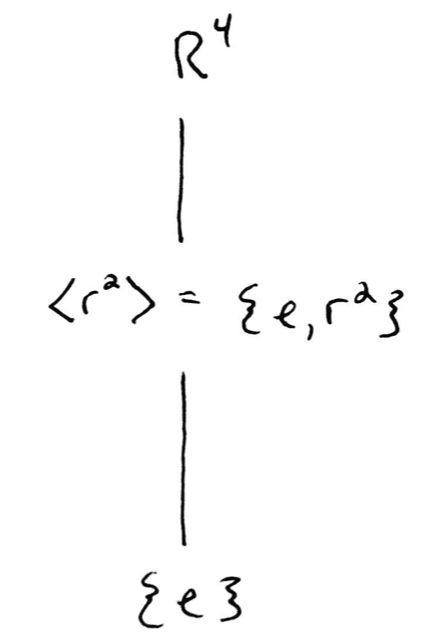
\includegraphics[height=2in]{latticeR4.png}
\end{center}

In general, subgroups of smaller order are towards the bottom of the lattice while larger subgroups are towards the top.  Moreover, an edge between to subgroups means that the smaller set is a subgroup of the larger set.

Let's see what we can do with $V_4=\{e,v,h,vh\}$.  Using an exhaustive search, we find that there are five subgroups:
\begin{itemize}
\item[] $\langle e \rangle = \{e\}$
\item[] $\langle h \rangle  = \{e,h\}$
\item[] $\langle v \rangle  = \{e.v\}$
\item[] $\langle vh \rangle  = \{e,vh\}$
\item[] $\langle v,h \rangle = \langle v,vh\rangle = \langle h, vh\rangle= \{e,v,h,vh\}=V_4$
\end{itemize}
For each subgroup above, we've used minimal generating sets to determine the group.  (Note that minimal generating sets are generating sets where we cannot remove any elements and still obtain the same group.  Two minimal generating sets for the same group do not have to have the same number of generators.)  In this case, we get the following subgroup lattice.

\begin{center}
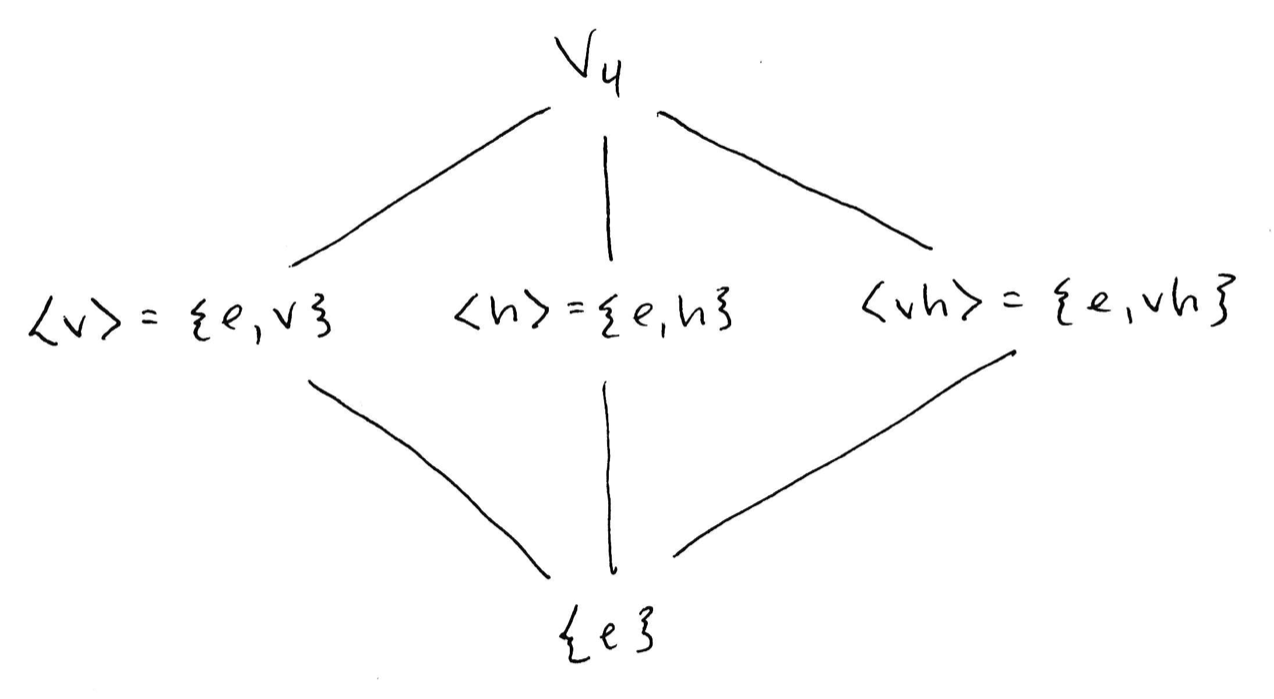
\includegraphics[height=2in]{latticeV4.png}
\end{center}

Notice that there are no edges among $\langle v\rangle, \langle h\rangle$, and $\langle vh\rangle$.  The reason for this is that none of these groups are subgroups of each other.  We already know that $R_4$ and $V_4$ are not isomorphic, but this becomes even more apparent if you compare their subgroup lattices.

\begin{problem}
What claims can be made about the subgroup lattices of two groups that are isomorphic? What claims can be made about the subgroup lattices of two groups that are not isomorphic?  What claims can be made about two groups if their subgroup lattices look nothing alike?  \emph{Hint:} The answers to two of these questions should be obvious, but the answer to the remaining question should be something like, ``we don't have enough information to make any claims."
\end{problem}

In the next few exercises, you are asked to create subgroup lattices.  As you do this, try to minimize the amount of work it takes to come up with all the subgroups.  In particular, I do \emph{not} recommend doing a full brute-force like we did for $R_4$. 

\begin{exercise}
Find all the subgroups of $R_5=\{e,r,r^2,r^3,r^4\}$ (where $r$ is rotation of a regular pentagon by $72^{\circ}$) and then draw the subgroup lattice for $R_5$.
\end{exercise}

\begin{exercise}
Find all the subgroups of $R_6=\{e,r,r^2,r^3,r^4,r^5\}$ (where $r$ is rotation of a regular hexagon by $60^{\circ}$) and then draw the subgroup lattice for $R_6$.
\end{exercise}

\begin{exercise}
Find all the subgroups of $D_3=\{e,r,r^2,s,sr,sr^2\}$ (where $r$ and $s$ are the usual actions) and then draw the subgroup lattice for $D_3$.
\end{exercise}

\begin{exercise}
Find all the subgroups of $D_4=\{e,r,r^2,r^3,s,sr,sr^2,sr^3\}$ (where $r$ and $s$ are the usual actions) and then draw the subgroup lattice for $D_4$.
\end{exercise}

\begin{exercise}
Find all the subgroups of $Q_8=\{1,-1,i,-i,j,-j,k,-k\}$ and then draw the subgroup lattice for $Q_8$.
\end{exercise}

Here are two final problems to conclude this section.

\begin{problem}
Several times we've referred to the fact that some subgroups are visible in a Cayley diagram for the parent group and some subgroups are not.  Suppose $(G,*)$ is a group and let $H\leq G$.  Can you describe a process for creating a Cayley diagram for $G$ that ``reveals" the subgroup $H$ inside of this Cayley diagram?
\end{problem}

\begin{problem}
Suppose $(G,*)$ is a finite group and let $H\leq G$.  Can you describe a process that ``reveals" the subgroup $H$ inside the group table for $G$?  Where will the clones for $H$ end up?
\end{problem}

\end{section}

\begin{section}{Revisiting Isomorphisms}

Suppose $(G_1,*)$ and $(G_2,\circ)$ are two groups.  Recall that $G_1$ and $G_2$ are isomorphic, written $G_1\cong G_2$, provided that we can choose generating sets for $G_1$ and $G_2$, respectively, so that the Cayley diagrams for both groups are identical (ignoring the labels on the vertices).  When two groups are isomorphic, it means that they have identical structure up to relabeling the names of the elements of the group.

One consequence of two groups being isomorphic is that there is a one-to-one correspondence between the elements of the group.  This correspondence is referred to as an isomorphism.  In other words, an isomorphism is a one-to-one and onto function that preserves the structure of the two groups.  

Having an isomorphism between two groups immediately implies that they have the same order, i.e., $|G_1|=|G_2|$ (see Theorem~\ref{thm:iso_same_order}).  However, it is extremely important to remember that two groups having the same order does \emph{not} imply that the two groups are isomorphic.  Said another way, having a one-to-one correspondence between two groups does not imply that the two groups are isomorphic.  They must also have the same structure!

\begin{exercise}
Provide an example of two groups that have the same order but are not isomorphic.
\end{exercise}

After we introduced groups tables, we also discussed the fact that $G_1\cong G_2$ exactly when we can arrange the rows and columns and color elements in such a way that the colorings for the two group tables agree (see Problem~\ref{prob:iso_same_group_table}).  The upshot of this is that if $G_1\cong G_2$, then
\begin{quotation}
\emph{the product of corresponding elements yields the corresponding result.}
\end{quotation}
This is the essence of what it means for two groups to have the same structure.  

Let's try to make a little more sense of this.  Suppose that $G_1\cong G_2$ and imagine we have arranged the rows and columns of their respective group tables and colored the elements in such a way that the colorings for the two group tables agree.  Now, let $x,y\in G_1$.  Then these two elements have corresponding elements in the group table for $G_2$, say $x'$ and $y'$, respectively.  In other words, $x$ and $x'$ have the same color while $y$ and $y'$ have the same color.  Since $G_1$ is closed under its binary operation $*$, there exists $z\in G_1$ such that $z=x*y$.  There must exist a $z'\in G_2$ such that $z'$ has the same color as $z$.  What must be true of $x'\circ y'$?  Since the two tables exhibit the same color pattern, it must the case that $z'=x'\circ y'$.  This is what is means for the product of corresponding elements to yield the corresponding result.  Below is a figure that depicts this phenomenon for group tables.

\begin{center}
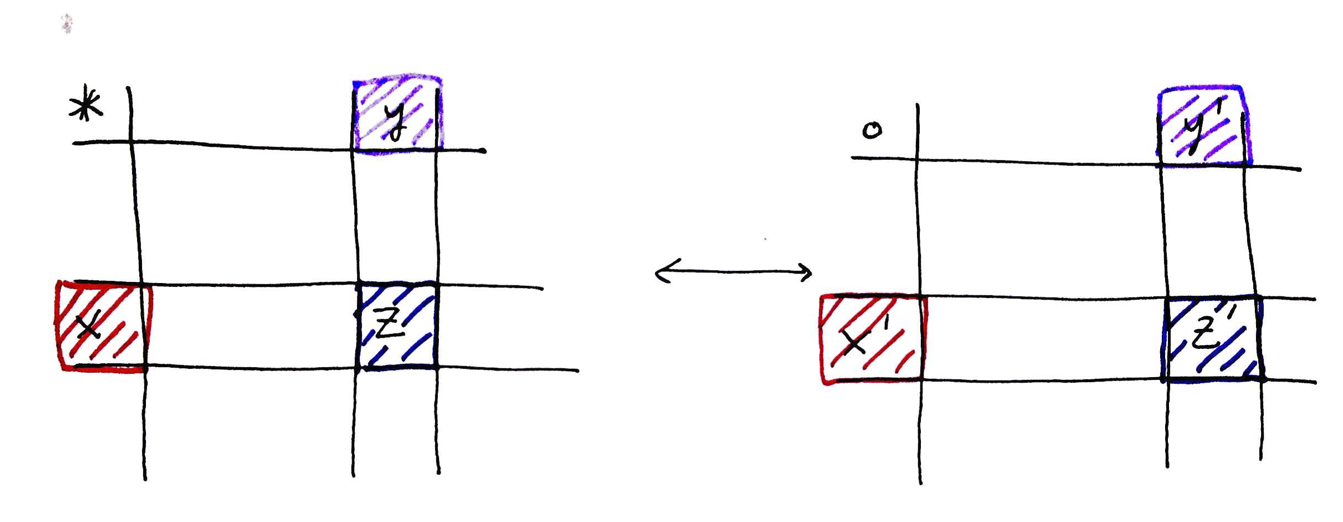
\includegraphics[width=5in]{isoGroupTables.png}
\end{center}

We can describe the isomorphism between $G_1$ and $G_2$ using a function.  Let $\phi:G_1\to G_2$ be the one-to-one and onto function that maps elements of $G_1$ to their corresponding elements in $G_2$.  Then $\phi(x)=x'$, $\phi(y)=y'$, and $\phi(z)=z'$.  Since $z'=x'\circ y'$, we can obtain
\[
\phi(x*y)=\phi(z)=z'=x'\circ y'=\phi(x)\circ \phi(y).
\]
In summary, it must be the case that 
\[
\phi(x*y)=\phi(x)\circ \phi(y).
\]
We are now prepared to state a formal definition of what it means for two groups to be isomorphic.

\begin{definition}\label{def:iso}
Let $(G_1,*)$ and $(G_2,\circ)$ be two groups.  Then $G_1$ is \textbf{isomorphic} to $G_2$, written $G_1\cong G_2$, if and only if there exists a one-to-one and onto function $\phi:G_1\to G_2$ such that
\begin{equation}\label{hom_property}
\phi(x*y)=\phi(x)\circ \phi(y).
\end{equation}
The function $\phi$ is referred to as an \textbf{isomorphism}.  Equation \ref{hom_property} is often referred to as the \textbf{homomorphic property}.
\end{definition}

You should definitely take a few minutes to convince yourself that the above definition agrees with our previous informal approach to isomorphisms.  For those of you that have had linear algebra, notice that our homomorphic property looks a lot like the requirement for a function on vector spaces to be a linear transformation.  Linear transformations preserve the algebraic structure of vector spaces while the homomorphic property is preserving the algebraic structure of groups.

We've seen several instances of two groups being isomorphic, but now that we have a formal definition, we can open the door to more possibilities.

\begin{problem}
Consider the groups $(\mathbb{R},+)$ and $(\mathbb{R}^+,\cdot)$, where $\mathbb{R}^+$ is the set of positive real numbers.  It turns out that these two groups are isomorphic, but this would be difficult to discover using our previous techniques because the groups are infinite.  Define $\phi:\mathbb{R}\to \mathbb{R}^+$ via $\phi(r)=e^r$ (where $e$ is the natural base).
\begin{enumerate}[label=\rm{(\alph*)}]
\item Briefly justify why $\phi$ is one-to-one and onto.
\item Prove that $\phi$ satisfies the homomorphic property.
\item Explain why parts (a) and (b) show that the two groups are isomorphic.
\end{enumerate}
\end{problem}

\begin{exercise}
For each of the following pairs of groups, determine whether the given function is an isomorphism from the first group to the second group.
\begin{enumerate}[label=\rm{(\alph*)}]
\item $(\mathbb{Z},+)$ and $(\mathbb{Z},+)$, $\phi(n)=n+1$.
\item $(\mathbb{Z},+)$ and $(\mathbb{Z},+)$, $\phi(n)=-n$.
\item $(\mathbb{Q},+)$ and $(\mathbb{Q},+)$, $\phi(x)=x/2$.
\end{enumerate}

\end{exercise}

\begin{problem}
Show that the groups $(\mathbb{Z},+)$ and $(2\mathbb{Z},+)$ are isomorphic.
\end{problem}

Perhaps one surprising consequence of the previous problem is that when dealing with infinite groups, a group can have a proper subgroup that it is isomorphic to.  Of course, this never happens with finite groups.

Once we know that two groups are isomorphic, there are lots of interesting things we can say.  The next theorem tells us that isomorphisms map the identity element of one group to the identity of the second group.  It was already clear that this was the case using our informal definition of isomorphic.  Prove the next theorem using Definition~\ref{def:iso}

\begin{theorem}\label{thm:hom_id}
Suppose $\phi:G_1\to G_2$ is an isomorphism from the group $(G_1,*)$ to the group $(G_2,\circ)$.  If $e$ and $e'$ are the identity elements of $G_1$ and $G_2$, respectively, then $\phi(e)=e'$.
\end{theorem}

\begin{theorem}\label{thm:hom_inverse}
Suppose $\phi:G_1\to G_2$ is an isomorphism from the group $(G_1,*)$ to the group $(G_2,\circ)$.   Then $\phi(g^{-1})=[\phi(g)]^{-1}$.
\end{theorem}

\begin{theorem}
Suppose $\phi:G_1\to G_2$ is an isomorphism from the group $(G_1,*)$ to the group $(G_2,\circ)$. If $G_1$ is abelian, then $G_2$ is abelian.
\end{theorem}

\begin{theorem}
Suppose $\phi:G_1\to G_2$ is an isomorphism from the group $(G_1,*)$ to the group $(G_2,\circ)$. Then the function $\phi^{-1}:G_2\to G_1$ is an isomorphism.
\end{theorem}

\begin{theorem}
Suppose $\phi:G_1\to G_2$ and $\psi:G_2\to G_3$ are isomorphisms from the groups $(G_1,*)$ to $(G_2,\circ)$ and $(G_2,\circ)$ to $(G_3,\star)$, respectively. Then the composite function $\psi\circ\phi$ is an isomorphism of $G_1$ and $G_3$.
\end{theorem}

\begin{theorem}
Let $\mathcal{G}$ be any nonempty collection of groups.  Then the relation $\cong$ of being isomorphic is an equivalence relation.
\end{theorem}

\begin{theorem}
Suppose $\phi:G_1\to G_2$ is an isomorphism from the group $(G_1,*)$ to the group $(G_2,\circ)$.  If $H\leq G_1$, then $\phi(H)\leq G_2$, where
\[
\phi(H):=\{y\in G_2:\text{there exists } h\in H\text{ such that }\phi(h)=y\}. 
\]
Note that $\phi(H)$ is called the \textbf{image} of $H$.
\end{theorem}

\begin{theorem}
Suppose $(G,*)$ is a group and let $g\in G$.  Define $\phi_g:G\to G$ via $\phi(x)=g^{-1}xg$.  Then $\phi_g$ is an isomorphism from $G$ to $G$.  Note that the map $\phi_g$ is called \textbf{conjugation} by $g$.
\end{theorem}

Now that you've proved the above theorems, it's a good idea to review the key themes.  If you were really paying attention, you may have noticed that in a few of the proofs, we did not use the fact that the function was one-to-one and onto despite assuming that the function was an isomorphism.

\begin{problem}
For which of the recent theorems could we remove the assumption that the function is one-to-one and onto and only assume that it satisfies the homomorphic property?  Such functions are called \textbf{homomorphisms} and will be the subject of a future chapter.
\end{problem}


\end{section}
\chapter{Families of Groups}
\label{chapter:families}
\thispagestyle{empty}

In this chapter we will explore a few families of groups, some of which we are already familiar with.

\begin{section}{Cyclic Groups}

Recall that if $G$ is a group and $g\in G$, then the \textbf{cyclic subgroup generated by $g$} is given by
\[
\langle g\rangle =\{g^k\mid k\in\mathbb{Z}\}.
\]
It is important to point out that $\langle g\rangle$ may be finite or infinite. In the finite case, the Cayley diagram with generator $g$ gives us a good indication of where the word ``cyclic" comes from (see Problem~\ref{prob:Cayley_cyclic}).  If there exists $g\in G$ such that $G=\langle g\rangle$, then we say that $G$ is a \textbf{cyclic group}.  

\begin{problem}
List all of the elements in each of the following cyclic subgroups.
\begin{enumerate}[label=\textrm{(\alph*)}]
\item $\langle r\rangle$, where $r\in D_3$
\item $\langle r\rangle$, where $r\in R_4$
\item $\langle rs\rangle$, where $rs\in D_4$
\item $\langle r^2\rangle$, where $r^2\in R_6$
\item $\langle i\rangle$, where $i\in Q_8$
\item $\langle 6\rangle$, where $6\in \mathbb{Z}$ and the operation is ordinary addition
\end{enumerate}
\end{problem}

\begin{problem}\label{prob:subgroup_generated_by_matrix}
Consider the group of invertible $2\times 2$ matrices with real number entries under the operation of matrix multiplication.  This group is denoted by $\mathrm{GL}_2(\mathbb{R})$.  List the elements in the cyclic subgroups generated by each of the following matrices.
\begin{multicols}{3}
\begin{enumerate}[label=\textrm{(\alph*)}]
\item $\begin{bmatrix} 0 & -1\\ -1 & 0\end{bmatrix}$
\item $\begin{bmatrix} 0 & -1\\ 1 & 0\end{bmatrix}$
\item $\begin{bmatrix} 2 & 0\\ 0 & 1\end{bmatrix}$
\end{enumerate}
\end{multicols}
\end{problem}

\begin{problem}\label{prob:cyclic_or_not}
Determine whether each of the following groups is cyclic.  
%Determine whether each of the groups from Problem~\ref{prob:computing_orders} is cyclic.
If the group is cyclic, find at least one generator.
\begin{multicols}{2}
\begin{enumerate}[label=\textrm{(\alph*)}]
\item $S_2$
\item $R_3$
\item $R_4$
\item $V_4$
\item $R_5$
\item $R_6$
\item $D_3$
\item $R_7$
\item $R_8$
\item $\Spin_{1\times 2}$
\item $D_4$
\item $Q_8$
\end{enumerate}
\end{multicols}
\end{problem}

\begin{problem}
Determine whether each of the following groups is cyclic.  If the group is cyclic, find at least one generator. If you believe that a group is not cyclic, try to sketch an argument.
\begin{multicols}{2}
\begin{enumerate}[label=\textrm{(\alph*)}]
\item $(\mathbb{Z},+)$
\item $(\mathbb{R},+)$
\item $(\mathbb{R}^+,\cdot)$
\item $(\{6^n\mid n\in\mathbb{Z}\},\cdot)$
\end{enumerate}
\end{multicols}
\begin{enumerate}
\item[(e)] $\textrm{GL}_2(\mathbb{R})$ under matrix multiplication
\item[(f)] $\{(\cos(\pi/4) +i\sin(\pi/4))^n\mid n\in \mathbb{Z}\}$ under multiplication of complex numbers
\end{enumerate}
\end{problem}

\begin{theorem}\label{thm:cyclic_implies_abelian}
If $G$ is a cyclic group, then $G$ is abelian.
\end{theorem}

\begin{problem}\label{prob:abelian_does_not_imply_cyclic}
Provide an example of a finite group that is abelian but not cyclic.
\end{problem}

\begin{problem}
Provide an example of an infinite group that is abelian but not cyclic.
\end{problem}

\begin{theorem}\label{thm:subgroup_generated_by_inverse}
If $G$ is a group and $g\in G$, then $\langle g\rangle=\langle g^{-1}\rangle$.
\end{theorem}

\begin{theorem}
If $G$ is a cyclic group such that $G$ has exactly one element that generates all of $G$, then the order of $G$ is at most order 2.   
\end{theorem}

\begin{theorem}
If $G$ is a group such that $G$ has no proper nontrivial subgroups, then $G$ is cyclic.
\end{theorem}

Recall that the order of a group $G$, denoted $|G|$, is the number of elements in $G$. We define the \textbf{order} of an element $g$, written $|g|$, to be the order of $\langle g\rangle$.  That is, $|g|=|\langle g\rangle|$.  It is clear that $G$ is cyclic with generator $g$ if and only if $|G|=|g|$.

\begin{problem}
What is the order of the identity in any group?
\end{problem}

\begin{problem}\label{prob:computing_orders}
Find the orders of each of the elements in each of the groups in Problem~\ref{prob:cyclic_or_not}.
\end{problem}

\begin{problem}
Consider the group $(\mathbb{Z},+)$.  What is the order of 1?  Are there any elements in $\mathbb{Z}$ with finite order?
\end{problem}

\begin{problem}
Find the order of each of the matrices in Problem~\ref{prob:subgroup_generated_by_matrix}.
\end{problem}

The next result follows immediately from Theorem~\ref{thm:subgroup_generated_by_inverse}.

\begin{theorem}
If $G$ is a group and $g\in G$, then $|g|=|g^{-1}|$.
\end{theorem}

The next result should look familiar and will come in handy a few times in this chapter. We'll take the result for granted and not worry about proving it.

\begin{theorem}[Division Algorithm]
If $n$ is a positive integer and $m$ is any integer, then there exist unique integers $q$ (called the \textbf{quotient}) and $r$ (called the \textbf{remainder}) such that $m=nq+r$, where $0\leq r<n$.
\end{theorem}

\begin{theorem}\label{thm:finite_group_finite_exponent}
Suppose $G$ is a group and let $g\in G$. The subgroup $\langle g\rangle$ is finite if and only if there exists $n\in\mathbb{N}$ such that $g^n=e$.\footnote{For the forward implication, if $\langle g\rangle$ is finite, then there exists distinct positive integers $i$ and $j$ such that $g^i=g^j$.  Can you find a useful way to rewrite this equation? For the reverse implication, let $m\in\mathbb{Z}$ and use the Division Algorithm with $m$ and $n$.}
\end{theorem}

\begin{corollary}\label{cor:finite_group_finite_exponent}
If $G$ is a finite group, then for all $g\in G$, there exists $n\in\mathbb{N}$ such that $g^n=e$.
\end{corollary}

\begin{theorem}
Suppose $G$ is a group and let $g\in G$ such that $\langle g\rangle$ is a finite group. If $n$ is the smallest positive integer such that $g^n=e$, then $\langle g\rangle = \{e, g, g^2, \ldots, g^{n-1}\}$ and this set contains $n$ distinct elements.\footnote{Note that Theorem~\ref{thm:finite_group_finite_exponent} together with the Well-Ordering Principle guarantees the existence of a smallest positive integer $n$ such that $g^n=e$. The claim that the set contains $n$ distinct elements is not immediate.  You need to argue that there are no repeats in the list. Choose distinct $i,j\in\{0,1,\ldots,n-1\}$ such that $i\neq j$ and then show that $g^i\neq g^j$.  Consider a proof by contradiction and try to contradict the minimality of $n$.}
\end{theorem}

The next result provides an extremely useful interpretation of the order of an element.

\begin{corollary}\label{cor:order_smallest_exponent}
If $G$ is a group and $g\in G$ such that $\langle g\rangle$ is a finite group, then the order of $g$ is the smallest positive integer $n$ such that $g^n=e$.
\end{corollary}

\begin{problem}\label{prob:Cayley_cyclic}
Suppose $G$ is a finite cyclic group such that $G=\langle g\rangle$. Using the generating set $\{g\}$, what does the Cayley diagram for $G$ look like?
\end{problem}

\begin{problem}
Suppose $G$ is a finite cyclic group of order $n$ with generator $g$.  If we write down the group table for $G$ using $e, g, g^2, \ldots, g^{n-1}$ as the labels for the rows and columns, are there any interesting patterns in the table?
\end{problem}

\begin{problem}\label{prob:finite_pos_exps}
Notice that in the definition for $\langle g\rangle$, we allow the exponents on $g$ to be negative.  Explain why we only need to use positive exponents when $\langle g\rangle$ is a finite group.
\end{problem}

The Division Algorithm should come in handy when proving the next theorem.

\begin{theorem}\label{thm:criterion_on_powers}
Suppose $G$ is a group and let $g\in G$ such that $|g|=n$.  Then $g^i=g^j$ if and only if $n$ divides $i-j$.
\end{theorem}

\begin{corollary}
Suppose $G$ is a group and let $g\in G$ such that $|g|=n$.  If $g^k=e$, then $n$ divides $k$.
\end{corollary}

Recall that for $n\geq3$, $R_n$ is the group of rotational symmetries of a regular $n$-gon, where the operation is composition of actions.

\begin{theorem}
For all $n\geq 3$, $R_n$ is cyclic.
\end{theorem}

\begin{theorem}\label{thm:finite_cyclic_groups}
Suppose $G$ is a finite cyclic group of order $n$.  Then $G$ is isomorphic to $R_n$ if $n\geq 3$, $S_2$ if $n=2$, and the trivial group if $n=1$.
\end{theorem}

Most of the previous results have involved finite cyclic groups.  What about infinite cyclic groups?

\begin{theorem}
Suppose $G$ is a group and let $g\in G$. The subgroup $\langle g\rangle$ is infinite if and only if each $g^k$ is distinct for all $k\in\mathbb{Z}$.\footnote{For the forward implication, try a proof by contradiction and suppose there exists integers $i$ and $j$ such that $g^i=g^j$.}
\end{theorem}

\begin{theorem}\label{thm:infinite_cyclic_groups}
If $G$ is an infinite cyclic group, then $G$ is isomorphic to $\mathbb{Z}$ (under the operation of addition).
\end{theorem}

The upshot of Theorems~\ref{thm:infinite_cyclic_groups} and \ref{thm:finite_cyclic_groups} is that up to isomorphism, we know exactly what all of the cyclic groups are.

We now turn our attention to two new groups. Recall that two integers are \textbf{relatively prime} if the only positive integer that divides both of them is 1.  That is, integers $n$ and $k$ are relatively prime if and only if $\gcd(n,k)=1$.

\begin{definition}\label{def:integers_modn}
Let $n\in\mathbb{N}$ and define the following sets.
\begin{enumerate}[label=\textrm{(\alph*)}]
\item $\mathbb{Z}_n:=\{0,1,\ldots,n-1\}$
\item $U_n:=\{k\in\mathbb{Z}_n\mid \gcd(n,k)=1\}$
\end{enumerate}
\end{definition}

\begin{example}
For example, $\mathbb{Z}_{12}=\{0,1,2,3,4,5,6,7,8,9,10,11\}$ while $U_{12}=\{1,5,7,11\}$ since 1, 5, 7, and 11 are the only elements in $\mathbb{Z}_{12}$ that are relatively prime to 12.
\end{example}

For each set in Definition~\ref{def:integers_modn}, the immediate goal is to determine a binary operation that will yield a group.  The key is to use modular arithmetic.  Let $n$ be a positive integer. To calculate the sum (respectively, product) of two integers modulo $n$ (we say ``mod $n$" for short), add (respectively, multiply) the two numbers and then find the remainder after dividing the sum (respectively, product) by $n$. For example, $4+9$ is $3$ mod $5$ since $13$ has remainder 3 when divided by 5.  Similarly, $4\cdot 9$ is 1 mod $5$ since 36 has remainder 1 when divided by 5. The hope is that these two operations turn $\mathbb{Z}_n$ and $U_n$ into groups.

We write $i\equiv j\pmod n$, and say ``$i$ is equivalent to $j$ modulo $n$" or ``$i$ is equal to $j$ modulo $n$", if $i$ and $j$ both have the same remainder when divided by $n$.  It is common to abbreviate ``modulo" as ``mod".  It is also common to write $i\equiv_n j$, or even $i=j$ if the context is perfectly clear.  

It is well-known, and not too hard to prove, that $\equiv_n$ is an equivalence relation on $\mathbb{Z}$.  The corresponding equivalence classes are called congruence classes.  The elements of a single congruence class are the integers that all have the same remainder when divided by $n$. According to the Division Algorithm, there are $n$ congruence classes modulo $n$, one for each of the remainders $0,1,\ldots, n-1$. We can think of $\mathbb{Z}_n$ as the set of canonical representatives of these equivalence classes.

\begin{theorem}\label{thm:mod_divisiblity}
Let $n$ be a positive integer and let $i,j\in\mathbb{Z}$. Then $i\equiv j\pmod n$ if and only if $n$ divides $i-j$.
\end{theorem}

The next result follows immediately from Theorems~\ref{thm:mod_divisiblity} and \ref{thm:criterion_on_powers}.

\begin{corollary}
Suppose $G$ is a group and let $g\in G$ such that $|g|=n$.  Then $g^i=g^j$ if and only if $i\equiv j\pmod n$.
\end{corollary}

\begin{theorem}
The set $\mathbb{Z}_n$ is a cyclic group under addition mod $n$.\footnote{There are two things to prove here.  First, you need to prove that $\mathbb{Z}_n$ is a group under addition mod $n$, and then you need to argue that the group is cyclic.}
\end{theorem}

\begin{theorem}
The set $U_n$ is an abelian group under multiplication mod $n$.\footnote{Like the previous theorem, there are two things to prove. First, prove that $U_n$ is a group under multiplication mod $n$, and then argue that the group is abelian.}
\end{theorem}

\begin{problem}
Consider $\mathbb{Z}_4$.
\begin{enumerate}[label=\textrm{(\alph*)}]
\item Find the group table for $\mathbb{Z}_4$.
\item Is $\mathbb{Z}_4$ cyclic? If so, list elements of $\mathbb{Z}_4$ that individually generate $\mathbb{Z}_4$.  If $\mathbb{Z}_4$ is not cyclic, explain why.
\item Is $\mathbb{Z}_4$ isomorphic to either of $R_4$ or $V_4$? Justify your answer.
\item Draw the subgroup lattice for $\mathbb{Z}_4$.
\end{enumerate}
\end{problem}

The next two problems illustrate that $U_n$ may or may not be cyclic.

\begin{problem}\label{prob:U10}
Consider $U_{10}=\{1,3,7,9\}$.
\begin{enumerate}[label=\textrm{(\alph*)}]
\item Find the group table for $U_{10}$.
\item Is $U_{10}$ cyclic? If so, list elements of $U_{10}$ that individually generate $U_{10}$.  If $U_{10}$ is not cyclic, explain why.
\item Is $U_{10}$ isomorphic to either of $R_4$ or $V_4$? Justify your answer.
\item Is $U_{10}$ isomorphic to $\mathbb{Z}_4$? Justify your answer.
\item Draw the subgroup lattice for $U_{10}$.
\end{enumerate}
\end{problem}

\begin{problem}\label{prob:U12}
Consider $U_{12}=\{1,5,7,11\}$.
\begin{enumerate}[label=\textrm{(\alph*)}]
\item Find the group table for $U_{12}$.
\item Is $U_{12}$ cyclic? If so, list elements of $U_{12}$ that individually generate $U_{12}$.  If $U_{12}$ is not cyclic, explain why.
\item Is $U_{12}$ isomorphic to either of $R_4$ or $V_4$? Justify your answer.
\item Draw the subgroup lattice for $U_{12}$.
\end{enumerate}
\end{problem}

The upshot of the next theorem is that for $n\geq 3$, $\mathbb{Z}_n$ is just the set of exponents in the set $R_n=\{e,r,r^2,\ldots,r^{n-1}\}$ (where $e=r^0$).

\begin{theorem}\label{thm:Zn_iso_to_Rn}
For $n\geq 3$, $\mathbb{Z}_n\cong R_n$. Moreover, $\mathbb{Z}_2\cong S_2$ and $\mathbb{Z}_1$ is isomorphic to the trivial group.
\end{theorem}

The next result can be thought of as a repackaging of Theorems~\ref{thm:finite_cyclic_groups} and \ref{thm:infinite_cyclic_groups}.

\begin{theorem}
Let $G$ be a cyclic group. If the order of $G$ is infinite, then $G$ is isomorphic to $\mathbb{Z}$. If $G$ has finite order $n$, then $G$ is isomorphic to $\mathbb{Z}_n$.
\end{theorem}

Now that we have a complete description of the cyclic groups, let's focus our attention on subgroups of cyclic groups.  

\begin{theorem}\label{thm:subgroups_of_cyclic_groups}
Suppose $G$ is a cyclic group. If $H\leq G$, then $H$ is also cyclic.
\end{theorem}

It turns out that for proper subgroups, the converse of Theorem~\ref{thm:subgroups_of_cyclic_groups} is not true.

\begin{problem}
Provide an example of a group $G$ such that $G$ is not cyclic, but all proper subgroups of $G$ are cyclic.
\end{problem}

The next result officially settles Problem~\ref{prob:nZ}\ref{prob:nZothers} and also provides a complete description of the subgroups of infinite cyclic groups up to isomorphism.

\begin{corollary}\label{cor:subgroups_of_Z}
The subgroups of $\mathbb{Z}$ are precisely the groups $n\mathbb{Z}$ for $n\in \mathbb{Z}$.
\end{corollary}

Let's further explore finite cyclic groups.

\begin{theorem}\label{thm:order_of_power}
If $G$ is a finite cyclic group with generator $g$ such that $|G|=n$, then for all $m\in\mathbb{Z}$, $\displaystyle |g^m|=\frac{n}{\gcd(n,m)}$.\footnote{By Corollary~\ref{cor:order_smallest_exponent}, the order of $g^m$ is the smallest positive exponent $k$ such that $(g^m)^k=e$. First, verify that $k=\frac{n}{\gcd(n,m)}$ has the desired property and then verify that it is the smallest such exponent.}
\end{theorem}

\begin{theorem}\label{thm:subgroups_gcd}
If $G$ is a finite cyclic group with generator $g$ such that $|G|=n$, then $\langle g^m\rangle=\langle g^k\rangle$ if and only if $\gcd(m,n)=\gcd(k,n)$.\footnote{Use Theorem~\ref{thm:order_of_power} for the forward implication. For the reverse implication, first prove that for all $m\in\mathbb{Z}$, $\langle g^m\rangle=\langle g^{\gcd(m,n)}\rangle$ by proving two set containments. To show $\langle g^m\rangle\subseteq \langle g^{\gcd(m,n)}\rangle$, use the fact that there exists an integer $q$ such that $m=q\cdot \gcd(m,n)$. For the reverse containment, you may freely use a fact known as Bezout's Lemma, which states that $\gcd(m,n)=nx+my$ for some integers $x$ and $y$.}
\end{theorem}

\begin{problem}
Suppose $G$ is a cyclic group of order 12 with generator $g$. 
\begin{enumerate}[label=\textrm{(\alph*)}]
\item Find the orders of each of the following elements: $g^2$, $g^7$, $g^8$.
\item Which elements of $G$ individually generate $G$?
\end{enumerate}
\end{problem}

\begin{corollary}\label{cor:generator_relatively_prime}
Suppose $G$ is a finite cyclic group with generator $g$ such that $|G|=n$. Then $\langle g\rangle=\langle g^k\rangle$ if and only if $n$ and $k$ are relatively prime. That is, $g^k$ generates $G$ if and only if $n$ and $k$ are relatively prime.
\end{corollary}

\begin{problem}
Theorem~\ref{thm:order_of_power}, Theorem~\ref{thm:subgroups_gcd}, and Corollary~\ref{cor:generator_relatively_prime} are written using multiplicative notation.  Rewrite both of these results using additive notation.
\end{problem}

\begin{problem}
Consider $\mathbb{Z}_{18}$.
\begin{enumerate}[label=\textrm{(\alph*)}]
\item Find all of the elements of $\mathbb{Z}_{18}$ that individually generate all of $\mathbb{Z}_{18}$.
\item Draw the subgroup lattice for $\mathbb{Z}_{18}$. For each subgroup, list the elements of the corresponding set.  Moreover, circle the elements in each subgroup that individually generate that subgroup.  For example, $\langle 2\rangle=\{0,2,4,6,8,10,12,14,16\}$. In this case, we should circle 2, 4, 8, 10, 14, and 16 since each of these elements individually generate $\langle 2\rangle$ and none of the remaining elements do.  I'll leave it to you to figure out why this is true.
\end{enumerate}
\end{problem}

\begin{problem}
Repeat the above exercise, but this time use $\mathbb{Z}_{12}$ instead of $\mathbb{Z}_{18}$.
\end{problem}

\begin{corollary}
If $G$ is a finite cyclic group such that $|G|=p$, where $p$ is prime, then $G$ has no proper nontrivial subgroups.
\end{corollary}

\begin{problem}
If there is exactly one group up to isomorphism of order $n$, then to what group are all the groups of order $n$ isomorphic?
\end{problem}

\begin{problem}
Suppose $G$ is a group and $x,y\in G$ such that $|x|=m$ and $|y|=n$. Is it true that $|xy|=mn$?  If this is true, provide a proof.  If this is not true, then provide a counterexample.
\end{problem}

The punchline of the next two theorems is Theorem~\ref{thm:special_abelian_implies_cyclic}.

\begin{theorem}
Suppose $G$ is a finite abelian group and let $x,y\in G$ such that $|x|=m$ and $|y|=n$. If $\gcd(m,n)=1$, then $|xy|=mn$.\footnote{\emph{Hint:} First, verify that $(xy)^{mn}=e$. Now, suppose $|xy|=k$. What do you immediately know about the relationship between $k$ and $mn$. Next, consider $(xy)^{kn}$. Argue that $m$ divides $kn$ and then argue that $m$ divides $k$. Similarly, $n$ divides $k$. Ultimately, conclude that $mn=k$.}
\end{theorem}

\begin{theorem}
Suppose $G$ is a finite abelian group. If $n$ is the maximal order among all elements in $G$, then the order of every element in $G$ divides $n$.\footnote{\emph{Hint:} Suppose $g\in G$ such that $|g|=n$. Let $h$ be an arbitrary element in $G$ such that $|h|=m$. You need to show that $m$ divides $n$. For sake of a contradiction, assume otherwise. Then there exists a prime $p$ whose multiplicity as a factor of $m$ exceeds that of $n$. Let $p^a$ be the highest power of $p$ in $m$ and $p^b$ be the highest power of $p$ in $n$, so $a>b$. Consider the elements $g^{p^a}$ and $h^{m/p^b}$.}
\end{theorem}

Recall that every cyclic group is abelian (see Theorem~\ref{thm:cyclic_implies_abelian}).  However, we know that not every abelian group is cyclic (see Problem~\ref{prob:abelian_does_not_imply_cyclic}).  The next theorem tells us that abelian groups with some additional properties are cyclic.

\begin{theorem}\label{thm:special_abelian_implies_cyclic}
If $G$ is a finite abelian group with at most one subgroup of any order, then $G$ is cyclic.\footnote{\emph{Hint:} Let $n$ be the maximal order among the elements of $G$ and let $g\in G$ be an element with order $n$. Prove that $G=\langle g\rangle$.}
\end{theorem}

\begin{problem}
Is the converse of Theorem~\ref{thm:special_abelian_implies_cyclic} true for finite groups?  That is, if $G$ is a finite cyclic group, does that imply that $G$ contains at most one subgroup of each order? If the answer is yes, then prove it.  Otherwise, provide a counterexample.
\end{problem}

We conclude this section with a couple interesting counting problems involving the number of generators of certain cyclic groups.

\begin{problem}
Let $p$ and $q$ be distinct primes. Find the number of generators of $\mathbb{Z}_{pq}$.
\end{problem}

\begin{problem}
Let $p$ be a prime. Find the number of generators of $\mathbb{Z}_{p^r}$, where $r$ is an integer greater than or equal to 1.
\end{problem}

\end{section}

\begin{section}{Dihedral Groups}

We can think of finite cyclic groups as groups that describe rotational symmetry.  In particular, $R_n$ is the group of rotational symmetries of a regular $n$-gon.  Dihedral groups are those groups that describe both rotational and reflectional symmetry of regular $n$-gons.

\begin{definition}\label{def:dihedral}
For $n\geq 3$, the \textbf{dihedral group} $D_n$ is defined to be the group consisting of the symmetry actions of a regular $n$-gon, where the operation is composition of actions.
\end{definition}

For example, as we've seen, $D_3$ and $D_4$ are the symmetry groups of equilateral triangles and squares, respectively.  The symmetry group of a regular pentagon is denoted by $D_5$.  It is a well-known fact from geometry that the composition of two reflections in the plane is a rotation by twice the angle between the reflecting lines.

\begin{theorem}
The group $D_n$ is a non-abelian group of order $2n$.
\end{theorem}

\begin{theorem}\label{thm:generators_Dn}
Fix $n\geq 3$ and consider $D_n$. Let $r$ be rotation clockwise by $360^{\circ}/n$  and let $s$ and $s'$ be any two adjacent reflections of a regular $n$-gon.  Then
\begin{enumerate}[label=\textrm{(\alph*)}]
\item $D_n=\langle r,s\rangle =\{\underbrace{e,r,r^2,\ldots, r^{n-1}}_{\text{rotations}},\underbrace{s,sr,sr^2,\ldots,sr^{n-1}}_{\text{reflections}}\}$ and
\item $D_n=\langle s,s'\rangle = \text{all possible products of }s\text{ and }s'$.
\end{enumerate}
\end{theorem}

The next result is an obvious corollary of Theorem~\ref{thm:generators_Dn}.

\begin{corollary}
For $n\geq 3$, $R_n\leq D_n$.
\end{corollary}

The following theorem generalizes many of the relations we have witnessed in the Cayley diagrams for the dihedral groups $D_3$ and $D_4$.

\begin{theorem}
Fix $n\geq 3$ and consider $D_n$. Let $r$ be rotation clockwise by $360^{\circ}/n$  and let $s$ and $s'$ be any two adjacent reflections of a regular $n$-gon.  Then the following relations hold.
\begin{enumerate}[label=\textrm{(\alph*)}]
\item $r^n = s^2 = (s')^2 =e$,
\item $r^{-k} = r^{n-k}$ (special case: $r^{-1}=r^{n-1}$),
\item $sr^k=r^{n-k}s$ (special case: $sr=r^{n-1}s$),
\item $\underbrace{ss's\cdots}_{n\text{ factors}}=\underbrace{s'ss'\cdots}_{n\text{ factors}}$.
\end{enumerate}
\end{theorem}

\begin{problem}
From Theorem~\ref{thm:generators_Dn}, we know
\[
D_n=\langle r,s\rangle =\{\underbrace{e,r,r^2,\ldots, r^{n-1}}_{\text{rotations}},\underbrace{s,sr,sr^2,\ldots,sr^{n-1}}_{\text{reflections}}\}.
\]
If you were to create the group table for $D_n$ so that the rows and columns of the table were labeled by $e,r,r^2,\ldots, r^{n-1},s,sr,sr^2,\ldots,sr^{n-1}$ (in exactly that order), do any patterns arise?  Where are the rotations? Where are the reflections?
\end{problem}

\begin{problem}
What does the Cayley diagram for $D_n$ look like if we use $\{r,s\}$ as the generating set?  What if we use $\{s,s'\}$ as the generating set?
\end{problem}

\end{section}

\begin{section}{Symmetric Groups}

Recall the groups $S_2$ and $S_3$ from Problems~\ref{prob:introducing_S2} and \ref{prob:introducing_S3}.  These groups act on two and three coins, respectively, that are in a row by rearranging their positions (but not flipping them over). These groups are examples of symmetric groups.  In general, the \textbf{symmetric group} on $n$ objects is the set of permutations that rearranges the $n$ objects.  The group operation is composition of permutations.  Let's be a little more formal.

\begin{definition}
A \textbf{permutation of a set $A$} is a function $\sigma:A\to A$ that is both one-to-one and onto.
\end{definition}

You should take a moment to convince yourself that the formal definition of a permutation agrees with the notion of rearranging the set of objects.  The do-nothing action is the identity permutation, i.e., $\sigma(a)=a$ for all $a\in A$.  There are many ways to represent a permutation.  One visual way is using \textbf{permutation diagrams}, which we will introduce via examples.

Consider the following diagrams:
\begin{multicols}{2}
\[\alpha=\begin{pdiag}{5}{1}
\put(0.2,2.3){{1}}\put(1.2,2.3){{2}}\put(2.2,2.3){{3}}\put(3.2,2.3){{4}}\put(4.2,2.3){{5}} 
\pdmap{1}{2}\pdmap{2}{3}\pdmap{3}{4}\pdmap{4}{5}\pdmap{5}{1}\pdendmapfill 
\end{pdiag}\]

\bigskip

\[\beta=\begin{pdiag}{5}{1}
\put(0.2,2.3){{1}}\put(1.2,2.3){{2}}\put(2.2,2.3){{3}}\put(3.2,2.3){{4}}\put(4.2,2.3){{5}} 
\pdmap{2}{4}\pdmap{4}{3}\pdmap{3}{2}\pdendmapfill 
\end{pdiag}\]

\[\sigma=\begin{pdiag}{5}{1}
\put(0.2,2.3){{1}}\put(1.2,2.3){{2}}\put(2.2,2.3){{3}}\put(3.2,2.3){{4}}\put(4.2,2.3){{5}} 
\pdtrans{1}{3}\pdmap{2}{5}\pdmap{5}{4}\pdmap{4}{2}\pdendmapfill 
\end{pdiag}\]

\bigskip

\[\gamma=\begin{pdiag}{5}{1}
\put(0.2,2.3){{1}}\put(1.2,2.3){{2}}\put(2.2,2.3){{3}}\put(3.2,2.3){{4}}\put(4.2,2.3){{5}}
\pdtrans{1}{5}\pdendmapfill 
\end{pdiag}\]
\end{multicols}
\noindent Each of these diagrams represents a permutation on five objects.  I've given the permutations the names $\alpha$, $\beta$, $\sigma$, and $\gamma$.  The intention is to read the diagrams from the top down.  The numbers labeling the nodes along the top are identifying position.  Following an edge from the top row of nodes to the bottom row of nodes tells us what position an object moves to.  It is important to remember that the numbers are referring to the position of an object, not the object itself.  For example, $\beta$ is the permutation that sends the object in the second position to the fourth position, the object in the third position to the second position, and the object in the fourth position to the third position.  Moreover, the permutation $\beta$ doesn't do anything to the objects in positions 1 and 5.

\begin{problem}
Describe in words what the permutations $\sigma$ and $\gamma$ do.
\end{problem}

\begin{problem}
Draw the permutation diagram for the do-nothing permutation on 5 objects.  This is called the \textbf{identity permutation}. What does the identity permutation diagram look like in general for arbitrary $n$?
\end{problem}

\begin{definition}
The set of all permutations on $n$ objects is denoted by $S_n$.
\end{definition}

\begin{problem}
Draw all the permutation diagrams for the permutations in $S_3$.
\end{problem}

\begin{problem}
How many distinct permutations are there in $S_4$?  How about $S_n$ for any $n\in \mathbb{N}$?
\end{problem}

If $S_n$ is going to be a group, we need to know how to compose permutations.  This is easy to do using the permutation diagrams.  Consider the permutations $\alpha$ and $\beta$ from earlier.  We can represent the composition $\alpha \circ \beta$ via

\bigskip

\[\alpha \circ \beta=\begin{pdiag}{5}{2}
\put(0.2,4.3){{1}}\put(1.2,4.3){{2}}\put(2.2,4.3){{3}}\put(3.2,4.3){{4}}\put(4.2,4.3){{5}} 
\pdname{\tiny \beta}\pdmap{2}{4}\pdmap{4}{3}\pdmap{3}{2}\pdendmapfill 
\pdname{\tiny \alpha}\pdmap{1}{2}\pdmap{2}{3}\pdmap{3}{4}\pdmap{4}{5}\pdmap{5}{1}\pdendmapfill 
\end{pdiag}=
\begin{pdiag}{5}{1}
\put(0.2,2.3){{1}}\put(1.2,2.3){{2}}\put(2.2,2.3){{3}}\put(3.2,2.3){{4}}\put(4.2,2.3){{5}} 
\pdmap{1}{2}\pdmap{2}{5}\pdmap{5}{1}\pdendmapfill 
\end{pdiag}.\]
\noindent As you can see by looking at the figure, to compose two permutations, you stack the one that goes first in the composition (e.g., $\beta$ in the example above) on top of the other and just follow the edges from the top through the middle to the bottom.  If you think about how function composition works, this is very natural.  The resulting permutation is determined by where we begin and where we end in the composition.

We already know that the order of composition matters for functions, and so it should matter for the composition of permutations. To make this crystal clear, let's compose $\alpha$ and $\beta$ in the opposite order.  We see that

\bigskip

\[\beta \circ \alpha=\begin{pdiag}{5}{2}
\put(0.2,4.3){{1}}\put(1.2,4.3){{2}}\put(2.2,4.3){{3}}\put(3.2,4.3){{4}}\put(4.2,4.3){{5}} 
\pdname{\tiny \alpha}\pdmap{1}{2}\pdmap{2}{3}\pdmap{3}{4}\pdmap{4}{5}\pdmap{5}{1}\pdendmapfill 
\pdname{\tiny \beta}\pdmap{2}{4}\pdmap{4}{3}\pdmap{3}{2}\pdendmapfill 
\end{pdiag}=
\begin{pdiag}{5}{1}
\put(0.2,2.3){{1}}\put(1.2,2.3){{2}}\put(2.2,2.3){{3}}\put(3.2,2.3){{4}}\put(4.2,2.3){{5}} 
\pdmap{1}{4}\pdmap{4}{5}\pdmap{5}{1}\pdendmapfill 
\end{pdiag}.\]

\noindent The moral of the story is that composition of permutations does not necessarily commute.

\begin{problem}
Consider $\alpha$, $\beta$, $\sigma$, and $\gamma$ from earlier.  Can you find a pair of permutations that do commute?  Can you identify any features about your diagrams that indicate why they commuted?
\end{problem}

\begin{problem}
Fix $n\in\mathbb{N}$.  Convince yourself that any $\rho\in S_n$ composed with the identity permutation (in either order) equals $\rho$.
\end{problem}

If $S_n$ is going to be a group, we need to know what the inverse of a permutation is.

\begin{problem}
Given a permutation $\rho\in S_n$, describe a method for constructing $\rho^{-1}$.  Briefly justify that $\rho \circ \rho^{-1}$ will yield the identity permutation.
\end{problem}

At this point, we have all the ingredients we need to prove that $S_n$ forms a group under composition of permutations.

\begin{theorem}
The set of permutations on $n$ objects forms a group under the operation of composition.  That is, $(S_n,\circ)$ is a group.  Moreover, $|S_n|=n!$.
\end{theorem}

Note that it is standard convention to omit the composition symbol when writing down compositions in $S_n$.  For example, we will simply write $\alpha\beta$ to denote $\alpha \circ \beta$.

Permutation diagrams are fun to play with, but we need a more efficient way of encoding information.  One way to do this is using \textbf{cycle notation}.  Consider $\alpha, \beta, \sigma$, and $\gamma$ in $S_{5}$ from the previous examples.  Below I have indicated what each permutation is equal to using cycle notation.

\begin{align*}\alpha=&\begin{pdiag}{5}{1} 
\pdmap{1}{2}\pdmap{2}{3}\pdmap{3}{4}\pdmap{4}{5}\pdmap{5}{1}\pdendmapfill 
\end{pdiag}=\ (1,2,3,4,5)\\
\\
\beta=&\begin{pdiag}{5}{1} 
\pdmap{2}{4}\pdmap{4}{3}\pdmap{3}{2}\pdendmapfill 
\end{pdiag}=\ (2,4,3)\\
\\
\sigma=&\begin{pdiag}{5}{1} 
\pdtrans{1}{3}\pdmap{2}{5}\pdmap{5}{4}\pdmap{4}{2}\pdendmapfill 
\end{pdiag}=\ (1,3)(2,5,4)\\
\\
\gamma=&\begin{pdiag}{5}{1} 
\pdtrans{1}{5}\pdendmapfill 
\end{pdiag}=\ (1,5)
\end{align*}
Each string of numbers enclosed by parentheses is called a \textbf{cycle} and if the string of numbers has length $k$, then we call it a $k$-cycle.  For example, $\alpha$ consists of a single 5-cycle, whereas $\sigma$ consists of one 2-cycle and one 3-cycle.  In the case of $\sigma$, we say that $\sigma$ is the product of two \textbf{disjoint cycles}.  

One observation that you hopefully made is that if an object in position $i$ remains unchanged, then we don't bother listing that number in the cycle notation.  However, if we wanted to, we could use the 1-cycle $(i)$ to denote this.  For example, we could write $\beta=(1)(2,4,3)(5)$.  In particular, we could denote the identity permutation in $S_5$ using $(1)(2)(3)(4)(5)$.  Yet, it is common to simply use $(1)$ to denote the identity in $S_n$ for all $n$.

Notice that the first number we choose to write down for a given cycle is arbitrary.  However, the numbers that follow are not negotiable.  Typically, we would use the smallest possible number first, but this is not necessary.  For example, the cycle $(2,4,7)$ could also be written as $(4,7,2)$ or $(7,2,4)$.

\begin{problem}\label{prob:S3-2}
Write down all 6 elements in $S_3$ using cycle notation.
\end{problem}

\begin{problem}\label{prob:S4}
Write down all 24 elements in $S_4$ using cycle notation.
\end{problem}

Suppose $\sigma\in S_n$.  Since $\sigma$ is one-to-one and onto, it is clear that it is possible to write $\sigma$ as a product of disjoint cycles such that each $i\in\{1,2,\ldots, n\}$ appears exactly once.

Let's see if we can figure out how to multiply elements of $S_n$ using cycle notation.  Consider the permutations $\alpha=(1,3,2)$ and $\beta=(3,4)$ in $S_4$.  To compute the composition $\alpha\beta=(1,3,2)(3,4)$, let's explore what happens in each position.  Since we are doing function composition, we should work our way from right to left.  Since 1 does not appear in the cycle notation for $\beta$, we know that $\beta(1)=1$ (i.e., $\beta$ maps 1 to 1).  Now, we see what $\alpha(1)=3$.  Thus, the composition $\alpha\beta$ maps 1 to 3 (since $\alpha\beta(1)=\alpha(\beta(1))=\alpha(1)=3$).  Next, we should return to $\beta$ and see what happens to 3---which is where we ended a moment ago.  We see that $\beta$ maps 3 to 4 and then $\alpha$ maps 4 to 4 (since 4 does not appear in the cycle notation for $\alpha$).  So, $\alpha\beta(3)=4$.  Continuing this way, we see that $\beta$ maps 4 to 3 and $\alpha$ maps 3 to 2, and so $\alpha\beta$ maps 4 to 2.  Lastly, since $\beta(2)=2$ and $\alpha(2)=1$, we have $\alpha\beta(2)=1$.  Putting this altogether, we see that $\alpha\beta=(1,3,4,2)$.  Now, you should try a few.  Things get a little trickier if the composition of two permutations results in a permutation consisting of more than a single cycle.

\begin{problem}
Consider $\alpha$, $\beta$, $\sigma$, and $\gamma$ for which we drew the permutation diagrams.  Using cycle notation, compute each of the following.
\begin{multicols}{2}
\begin{enumerate}[label=\textrm{(\alph*)}]
\item $\alpha\gamma$
\item $\alpha^2$
\item $\alpha^3$
\item $\alpha^4$
\item $\alpha^5$
\item $\sigma\alpha$
\item $\alpha^{-1}\sigma^{-1}$
\item $\beta^2$
\item $\beta^3$
\item $\beta\gamma\alpha$
\item $\sigma^3$
\item $\sigma^6$
\end{enumerate}
\end{multicols}
\end{problem}

\begin{problem}
Write down the group table for $S_3$ using cycle notation.
\end{problem}

In Problem~\ref{prob:S4}, one of the permutations you should have written down is $(1,2)(3,4)$.  This is a product of two disjoint 2-cycles.  It is worth pointing out that each cycle is a permutation in its own right.  That is, $(1,2)$ and $(3,4)$ are each permutations.  It just so happens that their composition does not ``simplify" any further.  Moreover, these two disjoint 2-cycles commute since $(1,2)(3,4)=(3,4)(1,2)$.  In fact, this phenomenon is always true.

\begin{theorem}
Suppose $\alpha$ and $\beta$ are two disjoint cycles.  Then $\alpha\beta=\beta\alpha$.  That is, products of disjoint cycles commute.
\end{theorem}

\begin{problem}
Compute the orders of all the elements in $S_3$.  See Problem~\ref{prob:S3-2}.
\end{problem}

\begin{problem}
Compute the orders of any twelve of the elements in $S_4$.  See Problem~\ref{prob:S4}.
\end{problem}

Computing the order of a permutation is fairly easy using cycle notation once we figure out how to do it for a single cycle.  In fact, you've probably already guessed at the following theorem.

\begin{theorem}
If $\alpha\in S_n$ such that $\alpha$ consists of a single $k$-cycle, then $|\alpha|=k$.
\end{theorem}

\begin{theorem}
Suppose $\alpha\in S_n$ such that $\alpha$ consists of $m$ disjoint cycles of lengths $k_1,\ldots, k_m$.  Then $|\alpha|=\lcm(k_1,\ldots, k_m)$.\footnote{Recall that $\lcm(k_1,\ldots, k_m)$ is the \textbf{least common multiple} of $\{k_1,\ldots, k_m\}$.} 
\end{theorem}

\begin{problem}
Is the previous theorem true if we do not require the cycles to be disjoint?  Justify your answer.
\end{problem}

\begin{problem}
What is the order of $(1,4,7)(2,5)(3,6,8,9)$?
\end{problem}

\begin{problem}
Draw the subgroup lattice for $S_3$.
\end{problem}

\begin{problem}
Now, using $(1,2)$ and $(1,2,3)$ as generators, draw the Cayley diagram for $S_3$.  Look familiar?
\end{problem}

\begin{problem}
Consider $S_3$.
\begin{enumerate}[label=\textrm{(\alph*)}]
\item Using $(1,2)$, $(1,3)$, and $(2,3)$ as generators, draw the Cayley diagram for $S_3$.
\item In the previous part, we used a generating set with three elements.  Is there a smaller generating set?  If so, what is it?
\end{enumerate}
\end{problem}

\begin{problem}
Recall that there are $4!=24$ permutations in $S_4$.    
\begin{enumerate}[label=\textrm{(\alph*)}]
\item Pick any 12 permutations from $S_4$ and verify that you can write them as words in the 2-cycles $(1,2), (1,3), (1,4), (2,3), (2,4),(3,4)$.  In most circumstances, your words will not consist of products of disjoint 2-cycles.  For example, the permutation $(1,2,3)$ can be decomposed into $(1,2)(2,3)$, which is a word consisting of two 2-cycles that happen to not be disjoint.
\item Using your same 12 permutations, verify that you can write them as words only in the 2-cycles $(1,2),(2,3),(3,4)$.
\end{enumerate}
By the way, it might take some trial and error to come up with a way to do this.  Moreover, there is more than one way to do it.
\end{problem}

As the previous exercises hinted at, the 2-cycles play a special role in the symmetric groups.  In fact, they have a special name.  A \textbf{transposition} is a single cycle of length 2.  In the special case that the transposition is of the form $(i,i+1)$, we call it an \textbf{adjacent transposition}.  For example, $(3,7)$ is a (non-adjacent) transposition while $(6,7)$ is an adjacent transposition.

It turns out that the set of transpositions in $S_n$ is a generating set for $S_n$.  In fact, the adjacent transpositions form an even smaller generating set for $S_n$.  To get some intuition, let's play with a few examples.

\begin{problem}
Try to write each of the following permutations as a product of transpositions.  You do not necessarily need to use adjacent transpositions.
\begin{enumerate}[label=\textrm{(\alph*)}]
\item $(3,1,5)$
\item $(2,4,6,8)$
\item $(3,1,5)(2,4,6,8)$
\item $(1,6)(2,5,3)$
\end{enumerate}
\end{problem}

The products you found in the previous exercise are called \textbf{transposition representations} of the given permutation.

\begin{problem}
Consider the arbitrary $k$-cycle $(a_1,a_2,\ldots, a_k)$ from $S_n$ (with $k\leq n$).  Find a way to write this permutation as a product of 2-cycles. 
\end{problem}

\begin{problem}
Consider the arbitrary 2-cycle $(a,b)$ from $S_n$.  Find a way to write this permutation as a product of adjacent 2-cycles.
\end{problem}

The previous two problems imply the following theorem.

\begin{theorem}
Consider $S_n$.
\begin{enumerate}[label=\textrm{(\alph*)}]
\item Every permutation in $S_n$ can be written as a product of transpositions.
\item Every permutation in $S_n$ can be written as a product of adjacent transpositions.
\end{enumerate}
\end{theorem}

\begin{corollary}
The set of transpositions (respectively, the set of adjacent transpositions) from $S_n$ forms a generating set for $S_n$.
\end{corollary}

It is important to point out that the transposition representation of a permutation is not unique.  That is, there are many words in the transpositions that will equal the same permutation.  However, as we shall see in the next section, given two transposition representations for the same permutation, the number of transpositions will have the same parity (i.e., even versus odd).

\begin{remark}
Here are two interesting facts that I will let you ponder on your own time.
\begin{enumerate}[label=\textrm{(\alph*)}]
\item The group of rigid motion symmetries for a cube is isomorphic to $S_4$.  To convince yourself of this fact, first prove that this group has 24 actions and then ponder the action of $S_4$ on the four long diagonals of a cube.
\item It turns out that you can generate $S_4$ with $(1,2)$ and $(1,2,3,4)$.  Moreover, you can arrange the Cayley diagram for $S_4$ with these generators on a truncated cube, which is depicted in Figure~\ref{fig:TruncatedCube}.  Try it. 
\end{enumerate}
\end{remark}

\begin{figure}[ht!]
\begin{center}
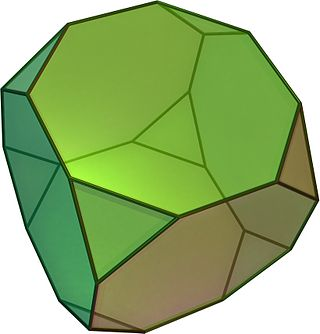
\includegraphics[width=2in]{TruncatedCube.jpg}
\end{center}
\caption{Truncated cube. [Image source: \href{https://en.wikipedia.org/wiki/Truncated_cube}{Wikipedia}]}\label{fig:TruncatedCube}
\end{figure}

It turns out that the subgroups of symmetric groups play an important role in group theory.

\begin{definition}
Every subgroup of a symmetric group is called a \textbf{permutation group}.
\end{definition}

The proof of the following theorem isn't too bad, but we'll take it for granted. After tinkering with a few examples, you should have enough intuition to see why the theorem is true and how a possible proof might go.

\begin{theorem}[Cayley's Theorem]
Every finite group is isomorphic to some permutation group.  In particular, if $G$ is a group of order $n$, then $G$ is isomorphic to a subgroup of $S_n$.
\end{theorem}

Cayley's Theorem guarantees that every finite group is isomorphic to a permutation group and it turns out that there is a rather simple algorithm for constructing the corresponding permutation group.  I'll briefly explain an example and then let you try a couple.

Consider the Klein four-group $V_4=\{e,v,h,vh\}$.  Recall that $V_4$ has the following group table.

\begin{center}
\begin{tabular}{c!{\vrule width 2pt}c|c|c|c}
$*$ & $e$ & $v$ & $h$ & $vh$ \\ \noalign{\hrule height 2pt}
$e$ & $e$ & $v$ & $h$ & $vh$ \\
\hline $v$ & $v$ & $e$ & $vh$ & $h$  \\
\hline $h$ & $h$ & $vh$ & $e$ & $v$\\
\hline $vh$ & $vh$ & $h$ & $v$ & $e$
\end{tabular}
\end{center}

If we number the elements $e,v,h,$ and $vh$ as $1,2,3,$ and $4$, respectively, then we obtain the following table.

\begin{center}
\begin{tabular}{c!{\vrule width 2pt}c|c|c|c}
 & $1$ & $2$ & $3$ & $4$ \\ \noalign{\hrule height 2pt}
$1$ & $1$ & $2$ & $3$ & $4$ \\
\hline $2$ & $2$ & $1$ & $4$ & $3$  \\
\hline $3$ & $3$ & $4$ & $1$ & $2$\\
\hline $4$ & $4$ & $3$ & $2$ & $1$
\end{tabular}
\end{center}

\noindent Comparing each of the four columns to the leftmost column, we can obtain the corresponding permutations.  In particular, we obtain
\begin{align*}
e&\leftrightarrow (1)\\
v&\leftrightarrow (1,2)(3,4)\\
h&\leftrightarrow (1,3)(2,4)\\
vh&\leftrightarrow(1,4)(2,3). 
\end{align*}
Do you see where these permutations came from?  The claim is that the set of permutations $\{(1),(1,2)(3,4),(1,3)(2,4),(1,4)(2,3)\}$ is isomorphic to $V_4$.  In this particular case, it's fairly clear that this is true.  However, it takes some work to prove that this process will always result in an isomorphic permutation group.  In fact, verifying the algorithm is essentially the proof of Cayley's Theorem. 

Since there are potentially many ways to rearrange the rows and columns of a given table, it should be clear that there are potentially many isomorphisms that could result from the algorithm described above.

Here's another way to obtain a permutation group that is isomorphic to a given group.  Let's consider $V_4$ again.  Recall that $V_4$ is a subset of $D_4$, which is the symmetry group for a square.  Alternatively, $V_4$ is the symmetry group for a non-square rectangle.  Label the corners of the rectangle 1, 2, 3, and 4 by starting in the upper left corner and continuing clockwise.  Recall that $v$ is the action that reflects the rectangle over the vertical midline.  The result of this action is that the corners labeled by 1 and 2 switch places and the corners labeled by 3 and 4 switch places.  Thus, $v$ corresponds to the permutation $(1,2)(3,4)$.  Similarly, $h$ swaps the corners labeled by 1 and 4 and the corners labeled by 2 and 3, and so $h$ corresponds to the permutation $(1,4)(2,3)$.  Notice that this is not the same answer we got earlier and that's okay as there may be many permutation representations for a given group.  Lastly, $vh$ rotates the rectangle $180^{\circ}$ which sends ends up swapping corners labeled 1 and 3 and swapping corners labeled by 2 and 4.  Therefore, $vh$ corresponds to the permutation $(1,3)(2,4)$.

\begin{problem}
Consider $D_4$.
\begin{enumerate}[label=\textrm{(\alph*)}]
\item Using the method outlined above, find a subgroup of $S_8$ that is isomorphic to $D_4$.
\item Label the corners of a square 1--4. Find a subgroup of $S_4$ that is isomorphic to $D_4$ by considering the natural action of $D_4$ on the labels on the corners of the square.
\end{enumerate}
\end{problem}

\begin{problem}
Consider $\mathbb{Z}_6$.
\begin{enumerate}[label=\textrm{(\alph*)}]
\item Using the method outlined earlier, find a subgroup of $S_6$ that is isomorphic to $\mathbb{Z}_6$.
\item Label the corners of a regular hexagon 1--6. Find a subgroup of $S_6$ that is isomorphic to $\mathbb{Z}_6$ by considering the natural action of $\mathbb{Z}_6$ on the labels on the corners of the hexagon.
\end{enumerate}
\end{problem}

\end{section}

\begin{section}{Alternating Groups}

In this section, we describe a special class of permutation groups.  To get started, let's play with a few exercises.

\begin{problem}
Write down every permutation in $S_3$ as a product of 2-cycles in the most efficient way you can find (i.e., use the fewest possible transpositions).  Now, write every permutation in $S_3$ as a product of adjacent 2-cycles, but don't worry about whether your decompositions are efficient.  Any observations about the number of transpositions you used in each case?  Think about even versus odd.
\end{problem}

\begin{theorem}
If $\alpha_1,\alpha_2,\ldots,\alpha_k$ is a collection of 2-cycles in $S_n$ such that $\alpha_1\alpha_2\cdots\alpha_k=(1)$, then $k$ must be even.
\end{theorem}

\begin{proof}
Suppose $\alpha_1,\alpha_2,\ldots,\alpha_k$ is a collection of 2-cycles in $S_n$ such that $\alpha_1\alpha_2\cdots\alpha_k=(1)$.  We need to show that $k$ is even. We proceed by strong induction. First, it is clear that the statement is not true when $k=1$, but is true when $k=2$. 

Now, assume that $k>2$ and if $j\leq k-1$ and we have a product of $j$ 2-cycles that equals the identity, then $j$ is even. Consider $\alpha_1\alpha_2$. The only possibilities are:
\begin{enumerate}
\item[(i)] $\alpha_1\alpha_2=(a,b)(a,b)$,
\item[(ii)] $\alpha_1\alpha_2=(a,b)(a,c)$,
\item[(iii)] $\alpha_1\alpha_2=(a,b)(c,d)$,
\item[(iv)] $\alpha_1\alpha_2=(a,b)(b,c)$.
\end{enumerate}
If case (i) happens, then
\[
(1)=\alpha_1\alpha_2\cdots\alpha_k=\alpha_3\alpha_4\cdots\alpha_k.
\]
Since the expression on the right consists of $k-2$ factors, $k-2$ must be even by induction, which implies that $k$ is even. Now, suppose we are in one of cases (ii), (iii), or (iv). Observe that:
\begin{enumerate}
\item[(ii)] $(a,b)(a,c)=(b,c)(a,b)$,
\item[(iii)] $(a,b)(c,d)=(c,d)(a,b)$,
\item[(iv)] $(a,b)(b,c)=(b,c)(a,c)$.
\end{enumerate}
In each case, we were able to move $a$ from the original left 2-cycle to a new right 2-cycle. That is, we were able to rewrite $\alpha_1\alpha_2$ so that $a$ does not appear in the left 2-cycle. Systematically repeat this process for the pairs $\alpha_2\alpha_3$, $\alpha_3\alpha_4$,\ldots, $\alpha_{k-1}\alpha_k$. If we ever encounter case (i) along the way, then we are done by induction. Otherwise, we are able to rewrite $\alpha_1\alpha_2\cdots\alpha_k$ so that $a$ only appears in the rightmost 2-cycle. But this implies that $\alpha_1\alpha_2\cdots\alpha_k$ does not fix $a$, which contradicts $\alpha_1\alpha_2\cdots\alpha_k =(1)$. This implies that at some point we must encounter case (i), and hence $k$ is even by induction.
\end{proof}

\begin{theorem}
If $\sigma\in S_n$, then every transposition representation of $\sigma$ has the same parity.
\end{theorem}

The previous theorem tells us that the following definition is well-defined.

\begin{definition}
A permutation is \textbf{even} (respectively, \textbf{odd}) if one of its transposition representations consists of an even (respectively, odd) number of transpositions.
\end{definition}

\begin{problem}
Classify all of the permutations in $S_3$ as even or odd.
\end{problem}

\begin{problem}
Classify all of the permutations in $S_4$ as even or odd.
\end{problem}

\begin{problem}
Determine whether $(1,4,2,3,5)$ is even or odd.  How about $(1,4,2,3,5)(7,9)$?
\end{problem}

\begin{problem}
Consider the arbitrary $k$-cycle $(a_1,a_2,\ldots, a_k)$ from $S_n$ (with $k\leq n$).  When will this cycle be odd versus even?  Briefly justify your answer. 
\end{problem}

\begin{problem}
Conjecture a statement about when a permutation will be even versus odd.  Briefly justify your answer.
\end{problem}

And finally, we are ready to introduce the alternating groups.

\begin{definition}
The set of all even permutations in $S_n$ is denoted by $A_n$ and is called the \textbf{alternating group}.
\end{definition}

Since we referred to $A_n$ as a group, it darn well better be a group!

\begin{theorem}
The set $A_n$ forms a group under composition of permutations and has order $n!/2$.\footnote{\emph{Hint:} To show that $A_n$ is a group, argue that $A_n$ is a subgroup of $S_n$ using the Two-Step Subgroup Test (see Theorem~\ref{thm:subgroup_criterion}). To show that $|A_n|=n!/2$, prove that the number of even permutations in $S_n$ is the same as the number of odd permutations in $S_n$.  Here is one way to accomplish this. Define $f:A_n\to S_n\setminus A_n$ via $f(\sigma)=(1,2)\sigma$.  Note that $S_n\setminus A_n$ is the set of odd permutations in $S_n$. Show that $f$ is a bijection.}
\end{theorem}

\begin{problem}
Find $A_3$.  What group is $A_3$ isomorphic to?
\end{problem}

\begin{problem}
Find $A_4$ and then draw its subgroup lattice. Is $A_4$ abelian?
\end{problem}

\begin{problem}
What is the order of $A_5$?  Is $A_5$ abelian?
\end{problem}

\begin{problem}
What are the possible orders for elements in $S_6$ and $A_6$?  What about $S_7$ and $A_7$?
\end{problem}

\begin{problem}
Does $A_8$ contain an element of order 15?  If so, find one.  If not, explain why no such element exists.
\end{problem}

\begin{remark}
Below are a few interesting facts about $A_4$ and $A_5$, which we will state without proof.
\begin{enumerate}[label=\textrm{(\alph*)}]
\item The group of rigid motion symmetries for a regular tetrahedron is isomorphic to $A_4$.
\item You can arrange the Cayley diagram for $A_4$ with generators $(1,2)(3,4)$ and $(2,3,4)$ on a truncated tetrahedron, which is depicted in Figure~\ref{fig:TruncatedTetrahedron}.
\item You can arrange the Cayley diagram for $A_5$ with generators $(1,2)(3,4)$ and $(1,2,3,4,5)$ on a truncated icosahedron, which is given in Figure~\ref{fig:TruncatedIcosahedron}.  You can also arrange the Cayley diagram for $A_5$ with generators $(1,2,3)$ and $(1,5)(2,4)$ on a truncated dodecahedron seen in Figure~\ref{fig:TruncatedDodecahedron}. 
\end{enumerate}
\end{remark}

\begin{figure}[!ht]
\begin{center}
\subcaptionbox{\label{fig:TruncatedTetrahedron}}[.3\textwidth]{
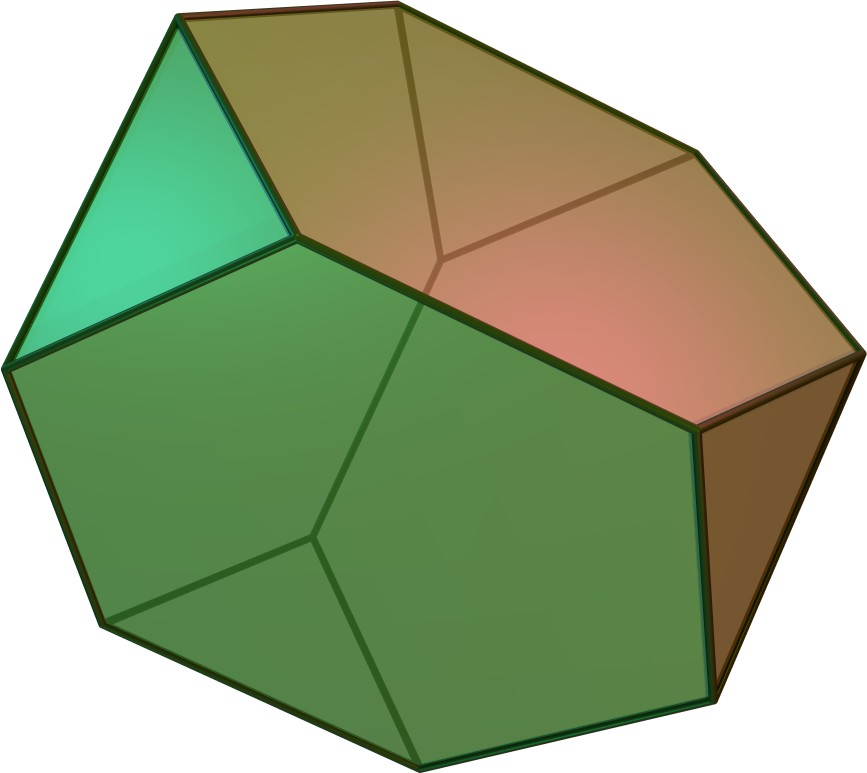
\includegraphics[width=1.5in]{TruncatedTetrahedron}
}
\subcaptionbox{\label{fig:TruncatedIcosahedron}}[.3\textwidth]{
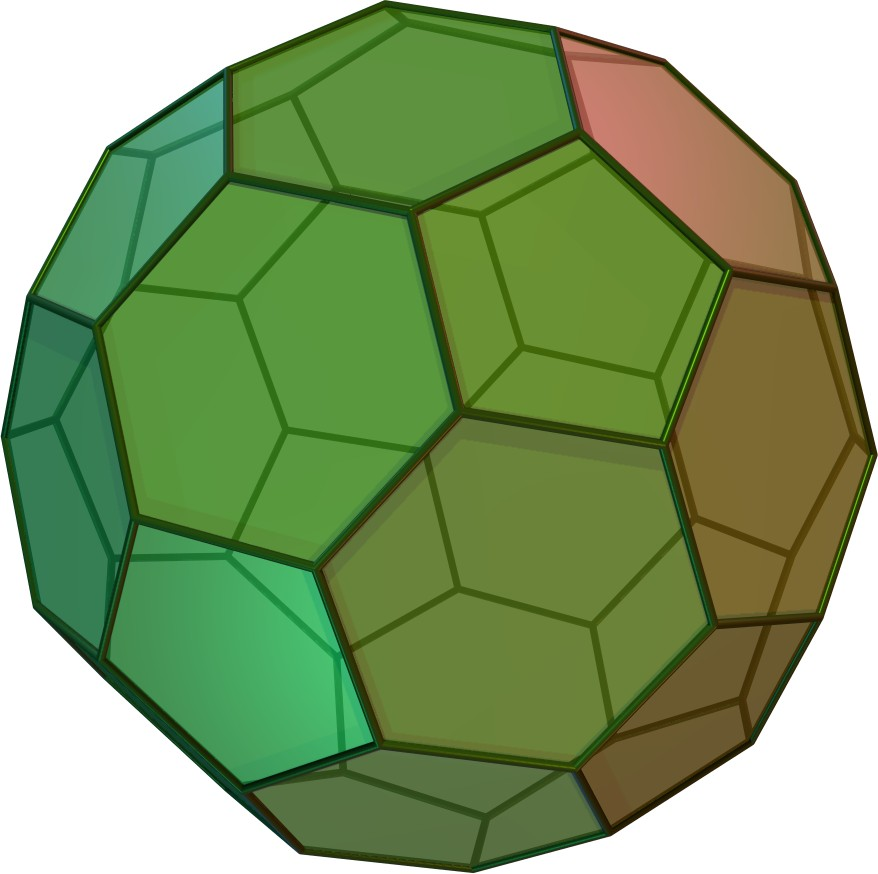
\includegraphics[width=1.5in]{TruncatedIcosahedron}}
\subcaptionbox{\label{fig:TruncatedDodecahedron}}[.3\textwidth]{
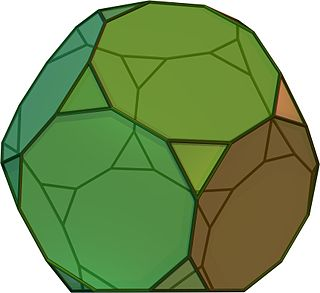
\includegraphics[width=1.5in]{TruncatedDodecahedron}}
\caption{Truncated tetrahedron, truncated icosahedron, and truncated dodecahedron. [Image source: \href{https://en.wikipedia.org/wiki/Truncated_tetrahedron}{Wikipedia}]}
\end{center}
\end{figure}

\end{section}
\chapter{Cosets, Lagrange's Theorem, and Normal Subgroups}
\label{chapter:cosets_lagrange_normal}
\thispagestyle{empty}

\begin{section}{Cosets}

Undoubtably, you've noticed numerous times that if $G$ is a group with $H\leq G$ and $g\in G$, then both $|H|$ and $|g|$ divide $|G|$.  The theorem that says this is always the case is called Lagrange's theorem and we'll prove it towards the end of this chapter.  We begin with a definition.

\begin{definition}
Let $G$ be a group and let $H\leq G$ and $a\in G$.  The subsets
\[
aH:=\{ah\mid h\in H\}
\]
and
\[
Ha:=\{ha\mid h\in H\}
\]
are called the \textbf{left} and \textbf{right cosets of $H$ containing $a$}, respectively.
\end{definition}

To gain some insight, let's tinker with an example.  Consider the dihedral group $D_3=\langle r,s\rangle$ and let $H=\langle s\rangle\leq D_3$.  To compute the right cosets of $H$, we need to multiply all of the elements of $H$ on the right by the elements of $G$.  We see that
\begin{align*}
& He =\{ee,se\}=\{e,s\}=H\\
& Hr=\{er,sr\}=\{r,sr\}\\
& Hr^2=\{er^2,sr^2\}=\{r^2,rs\}\\
& Hs=\{es,ss\}=\{s,e\}=H\\
& Hsr=\{esr,ssr\}=\{sr,r\}\\
& Hrs=\{ers,srs\}=\{rs,ssr^2\}=\{rs,r^2\}.
\end{align*}
Despite the fact that we made six calculations (one for each element in $D_3$), if we scan the list, we see that there are only 3 distinct cosets, namely
\begin{align*}
& H=He=Hs=\{e,s\}\\
& Hr=Hsr=\{r,sr\}\\
& Hr^2=Hrs=\{r^2,rs\}.
\end{align*}
We can make a few more observations.  First, the resulting cosets formed a partition of $D_3$.  That is, every element of $D_3$ appears in exactly one coset.  Moreover, all the cosets are the same size---two elements in each coset in this case.  Lastly, each coset can be named in multiple ways.  In particular, the elements of the coset are exactly the elements of $D_3$ we multiplied $H$ by.  For example, $Hr=Hsr$ and the elements of this coset are $r$ and $sr$.  Shortly, we will see that these observations hold, in general.

Here is another significant observation we can make.  Consider the Cayley diagram for $D_3$ with generating set $\{r,s\}$ that is given in Figure~\ref{fig:D3_repeat}. Given this Cayley diagram, we can visualize the subgroup $H$ and its clones.  Moreover, $H$ and its clones are exactly the 3 right cosets of $H$.  We'll see that, in general, the \emph{right} cosets of a given subgroup are always the subgroup and its clones (see Problem~\ref{prob:RightCosetsClones}).

\tikzstyle{vert} = [circle, draw, fill=grey,inner sep=0pt, minimum size=8mm]
\tikzstyle{h} = [draw,very  thick, blue,stealth-stealth]
\tikzstyle{r} = [draw, very thick, red,-stealth]

\begin{figure}[!ht]
\centering
\begin{tikzpicture}[scale=.75,auto]
\node (e) at (90:2) [vert] {$e$};
\node (r) at (-30:2) [vert] {$r$};
\node (rr) at (210:2) [vert] {$r^2$};
\node (h) at (90:4) [vert] {$s$};
\node (hr) at (210:4) [vert] {$rs$};
\node (hrr) at (-30:4) [vert] {$sr$};
\draw [r] (e) to [bend left] (r);
\draw [r] (r) to [bend left] (rr);
\draw [r] (rr) to [bend left] (e);
\draw [r] (h) to [bend right] (hr);
\draw [r] (hr) to [bend right] (hrr);
\draw [r] (hrr) to [bend right] (h);
\draw [h] (e) to (h);
\draw [h] (r) to (hrr);
\draw [h] (rr) to (hr);
\end{tikzpicture}
\caption{Cayley diagram for $D_3$ with generating set $\{r,s\}$.}
\label{fig:D3_repeat}
\end{figure}

\begin{exercise}\label{exer:left_cosets_D3}
Consider the group $D_3$.  Find all the left cosets for $H=\langle s\rangle$.  Are they the same as the right cosets?  Are they the same as the subgroup $H$ and its clones that we can see in the Cayley graph for $D_3$ with generating set $\{r,s\}$?
\end{exercise}

As the previous exercise indicates, the collections of left and right cosets may not be the same and when they are not the same, the subgroup and its clones do not coincide with the left cosets.

You might be thinking that somehow right cosets are ``better" than left cosets since we were able to visualize them in the Cayley graph.  However, this is just a consequence of our convention of composing actions from right to left.  If we had adopted a left to right convention, then we would be able to visualize the left cosets in Cayley diagrams.  

Computing left and right cosets using a group table is fairly easy.  Hopefully, you figured out in Exercise~\ref{exer:left_cosets_D3} that the left cosets of $H=\langle s\rangle$ in $D_3$ are $H=\{e,s\}$, $srH=\{r^2,sr\}$, and $rsH=\{r,rs\}$.  Now, consider the following group table for $D_3$ that has the rows and columns arranged according to the left cosets of $H$.

\begin{center}
\begin{tabu}{c|[2pt]c|c|c|c|c|c}
$*$ & $e$ & $s$ & $sr$ & $r^2$ & $rs$ & $r$ \\ \tabucline[2pt]{-}
$e$ & $e$ & $s$ & $sr$ & $r^2$ & $rs$ & $r$\\
\hline $s$ & $s$ & $e$ & $r$ & $rs$ & $r^2$ & $sr$ \\
\hline $sr$ & $sr$ & $r^2$ & $e$ & $s$ & $r$ & $rs$\\
\hline $r^2$ & $r^2$ & $sr$ & $rs$ & $r$ & $s$ & $e$\\
\hline $rs$ & $rs$ & $r$ & $r^2$ & $sr$ & $e$ & $s$\\
\hline $r$ & $r$ & $rs$ & $s$ & $e$ & $sr$ & $r^2$\\
\end{tabu}
\end{center}
The left coset $srH$ must appear in the row labeled by $sr$ and in the columns labeled by the elements of $H=\{e,s\}$.  We've depicted this below.

\begin{center}
\begin{tabu}{c|[2pt]c|c|c|c|c|c}
$*$ & \cellcolor{lightgray}$e$ & \cellcolor{lightgray}$s$ & $sr$ & $r^2$ & $rs$ & $r$ \\ \tabucline[2pt]{-}
$e$ & $e$ & $s$ & $sr$ & $r^2$ & $rs$ & $r$\\
\hline $s$ & $s$ & $e$ & $r$ & $rs$ & $r^2$ & $sr$ \\
\hline \cellcolor{lightgray}$sr$ & \cellcolor{blue}$sr$ & \cellcolor{blue}$r^2$ & $e$ & $s$ & $r$ & $rs$\\
\hline $r^2$ & $r^2$ & $sr$ & $rs$ & $r$ & $s$ & $e$\\
\hline $rs$ & $rs$ & $r$ & $r^2$ & $sr$ & $e$ & $s$\\
\hline $r$ & $r$ & $rs$ & $s$ & $e$ & $sr$ & $r^2$\\
\end{tabu}
\end{center}
On the other hand, the right coset $Hsr$ must appear in the column labeled by $sr$ and the rows labeled by the elements of $H=\{e,s\}$:
\begin{center}
\begin{tabu}{c|[2pt]c|c|c|c|c|c}
$*$ & $e$ & $s$ & \cellcolor{lightgray}$sr$ & $r^2$ & $rs$ & $r$ \\ \tabucline[2pt]{-}
\cellcolor{lightgray}$e$ & $e$ & $s$ & \cellcolor{blue}$sr$ & $r^2$ & $rs$ & $r$\\
\hline \cellcolor{lightgray}$s$ & $s$ & $e$ & \cellcolor{blue}$r$ & $rs$ & $r^2$ & $sr$ \\
\hline $sr$ & $sr$ & $r^2$ & $e$ & $s$ & $r$ & $rs$\\
\hline $r^2$ & $r^2$ & $sr$ & $rs$ & $r$ & $s$ & $e$\\
\hline $rs$ & $rs$ & $r$ & $r^2$ & $sr$ & $e$ & $s$\\
\hline $r$ & $r$ & $rs$ & $s$ & $e$ & $sr$ & $r^2$\\
\end{tabu}
\end{center}
As we can see from the tables, $srH\neq Hsr$ since $\{sr,r^2\}\neq \{sr,r\}$.  If we color the entire group table for $D_3$ according to which \emph{left} coset an element belongs to, we get the following.
 
\begin{center}
\begin{tabu}{c|[2pt]c|c|c|c|c|c}
$*$ & $e$ & $s$ & $sr$ & $r^2$ & $rs$ & $r$ \\ \tabucline[2pt]{-}
$e$ & \cellcolor{red}$e$ & \cellcolor{red}$s$ & \cellcolor{blue}$sr$ & \cellcolor{blue}$r^2$ & \cellcolor{green}$rs$ & \cellcolor{green}$r$\\
\hline $s$ & \cellcolor{red}$s$ & \cellcolor{red}$e$ & \cellcolor{green}$r$ & \cellcolor{green}$rs$ & \cellcolor{blue}$r^2$ & \cellcolor{blue}$sr$ \\
\hline $sr$ & \cellcolor{blue}$sr$ & \cellcolor{blue}$r^2$ & \cellcolor{red}$e$ & \cellcolor{red}$s$ & \cellcolor{green}$r$ & \cellcolor{green}$rs$\\
\hline $r^2$ & \cellcolor{blue}$r^2$ & \cellcolor{blue}$sr$ & \cellcolor{green}$rs$ & \cellcolor{green}$r$ & \cellcolor{red}$s$ & \cellcolor{red}$e$\\
\hline $rs$ & \cellcolor{green}$rs$ & \cellcolor{green}$r$ & \cellcolor{blue}$r^2$ & \cellcolor{blue}$sr$ & \cellcolor{red}$e$ & \cellcolor{red}$s$\\
\hline $r$ & \cellcolor{green}$r$ & \cellcolor{green}$rs$ & \cellcolor{red}$s$ & \cellcolor{red}$e$ & \cellcolor{blue}$sr$ & \cellcolor{blue}$r^2$\\
\end{tabu}
\end{center}
We would get a similar table (but in this case, not identical) if we colored the elements according to the right cosets.

Let's tackle a few more examples.

\begin{exercise}\label{exer:normal_in_D3}
Consider $D_3$ and let $K=\langle r\rangle$.  
\begin{enumerate}[label=\rm{(\alph*)}]
\item Find all of the left cosets of $K$ and then find all of the right cosets of $K$ in $D_3$.  Any observations?
\item Write down the group table for $D_3$, but this time arrange the rows and columns according to the left cosets for $K$.  Color the entire table according to which \emph{left} coset an element belongs to.  Can you visualize the observations you made in part (a)?
\end{enumerate}
\end{exercise}

\begin{exercise}\label{exer:normal_in_Q8}
Consider $Q_8$.  Let $H=\langle i\rangle$ and $K=\langle -1\rangle$.
\begin{enumerate}[label=\rm{(\alph*)}]
\item Find all of the left cosets of $H$ and all of the right cosets of $H$ in $Q_8$.  
\item Write down the group table for $Q_8$ so that rows and columns are arranged according to the left cosets for $H$.  Color the entire table according to which \emph{left} coset an element belongs to.
\item Find all of the left cosets of $K$ and all of the right cosets of $K$ in $Q_8$.
\item Write down the group table for $Q_8$ so that rows and columns are arranged according to the left cosets for $K$.  Color the entire table according to which \emph{left} coset an element belongs to.
\end{enumerate}
\end{exercise}

\begin{exercise}
Consider $S_4$.  Find all of the left cosets and all of the right cosets of $A_4$ in $S_4$. Instead of doing brute-force, try to be clever. \emph{Hint:} What happens when you compose two even permutations versus an even permutation and an odd permutation?
\end{exercise}

\begin{exercise}
Consider $\mathbb{Z}_8$.  Find all of the left cosets and all of the right cosets of $\langle 4\rangle$ in $\mathbb{Z}_8$. Why do you know the left and right cosets are the same without actually verifying?
\end{exercise}

\begin{exercise}
Consider $(\mathbb{Z},+)$.  Find all of the left cosets and all of the right cosets of $3\mathbb{Z}$ in $\mathbb{Z}$. Why do you know the left and right cosets are the same without actually verifying?
\end{exercise}

\begin{theorem}
Let $G$ be a group and let $H\leq G$. If $G$ is abelian, then for all $a\in G$, $aH=Ha$.  That is, if $G$ is abelian, then the left cosets of $H$ are the same as the right cosets of $H$.
\end{theorem}

Exercises~\ref{exer:left_cosets_D3} and \ref{exer:normal_in_D3} illustrate that if a group is non-abelian, then the cosets of a subgroup may or may not coincide.  That is, knowing that the group is non-abelian is not enough to determine whether the left and right cosets are different.

Now that we've played with a few examples, let's make a few general observations.

\begin{theorem}\label{thm:coset_representative}
Let $G$ be a group and let $H\leq G$.
\begin{enumerate}[label=\rm{(\alph*)}]
\item If $a\in G$, then $a\in aH$ (respectively, $Ha$).
\item If $b\in aH$ (respectively, $Ha$), then $aH=bH$ (respectively, $Ha=Hb$).
\item If $a\in H$, then $aH=H=Ha$.
\item If $a\notin H$, then for all $h\in H$, $ah\notin H$ (respectively, $ha \notin H$).
\end{enumerate}
\end{theorem}

The upshot of part (b) of Theorem~\ref{thm:coset_representative} is that cosets can have different names.  In particular, if $b$ is an element of the left coset $aH$, then we could have just as easily called the coset by the name $bH$.  In this case, both $a$ and $b$ are called \textbf{coset representatives}.

In all of the examples we've seen so far, the left and right cosets partitioned $G$ into equal-sized chunks.  We need to prove that this is true in general.  To prove that the cosets form a partition, we'll define an appropriate equivalence relation.

\begin{theorem}
Let $G$ be a group and let $H\leq G$.  Define $\sim_L$ and $\sim_R$ via 
\begin{center}
$a\sim_L b$ if and only if $a^{-1}b\in H$
\end{center}
and
\begin{center}
$a\sim_R b$ if and only if $ab^{-1}\in H$.
\end{center}
Then both $\sim_L$ and $\sim_R$ are equivalence relations.\footnote{You only need to prove that either $\sim_L$ or $\sim_R$ is an equivalence relation as the proof for the other is similar.}
\end{theorem}

\begin{problem}
If $[a]_{\sim_L}$ (respectively, $[a]_{\sim_R}$) denotes the equivalence class of $a$ under $\sim_L$ (respectively, $\sim_R$), what is $[a]_{\sim_L}$ (respectively, $[a]_{\sim_R}$)?  \emph{Hint:} It's got something to do with cosets.
\end{problem}

\begin{corollary}
If $G$ is a group and $H\leq G$, then the left (respectively, right) cosets of $H$ form a partition of $G$.
\end{corollary}

Next, we argue that all of the cosets have the same size.

\begin{theorem}
Let $G$ be a group, $H\leq G$, and $a\in G$.  Define $\phi:H\to aH$ via $\phi(h)=ah$.  Then $\phi$ is one-to-one and onto.
\end{theorem}

\begin{corollary}\label{cor:cosets_same_size}
Let $G$ be a group and let $H\leq G$.  Then all of the left and right cosets of $H$ are the same size as $H$.  In other words $\#(aH)=|H|=\#(Ha)$ for all $a\in G$.\footnote{As you probably expect, $\#(aH)$ denotes the size of $aH$. Note that everything works out just fine even if $H$ has infinite order.}
\end{corollary}

The final result of this chapter verifies that the clones of a subgroup in a Cayley diagram coincide with the right cosets of the subgroup.

\begin{problem}\label{prob:RightCosetsClones}
Let $G$ be a finite group with generating set $S$ and let $H$ be a proper subgroup of $G$ and suppose we can visualize the subgroup for $H$ in the Cayley diagram for $G$ using $S$ as the generating set. 
\begin{enumerate}[label=\rm{(\alph*)}]
\item If $g\in G$, verify that the right coset $Hg$ is a clone of $G$. \emph{Hint:} Suppose $s\in S$ and $h_1, h_2\in H$ such that there is an arrow labeled by $s$ that points from $h_1$ to $h_2$.  Argue that there is an arrow labeled by $s$ pointing from $h_1g$ to $h_2g$.
\item If $C$ is a clone of $H$, prove that $C$ is a right coset of $H$.
\end{enumerate}
\end{problem}

\end{section}

\begin{section}{Lagrange's Theorem}

We're finally ready to state Lagrange's Theorem, which is named after the Italian born mathematician Joseph Louis Lagrange.  It turns out that Lagrange did not actually prove the theorem that is named after him.  The theorem was actually proved by Carl Friedrich Gauss in 1801.

\begin{theorem}[Lagrange's Theorem]
Let $G$ be a finite group and let $H\leq G$.  Then $|H|$ divides $|G|$.
\end{theorem}

This simple sounding theorem is extremely powerful.  One consequence is that groups and subgroups have a fairly rigid structure.  Suppose $G$ is a finite group and let $H\leq G$.  Since $G$ is finite, there must be a finite number of distinct left cosets, say $H, a_2H, \ldots, a_{n}H$.  Corollary~\ref{cor:cosets_same_size} tells us that each of these cosets is the same size.  In particular, Lagrange's Theorem implies that for each $i\in\{1,\ldots, n\}$, $|a_iH|=|G|/n$, or equivalently $n=|G|/|a_iH|$.  This is depicted in Figure~\ref{fig:Lagrange}, where each rectangle represents a coset and we've labeled a single coset representative in each case.

\begin{figure}[!ht]
\centering
\begin{tikzpicture}[scale=1.6]
\draw (0,0) -- (5,0) -- (5,2) -- (0,2) -- (0,0);
\draw (1,0) -- (1,2);
\draw (2,0) -- (2,2);
\draw (4,0) -- (4,2);
\draw[fill=black] (.2,1.75) circle (1pt) node[below right] {$e$};
\draw[fill=black] (1.2,1.75) circle (1pt) node[below right] {$a_2$};
\draw[fill=black] (4.2,1.75) circle (1pt) node[below right] {$a_{n}$};
\node at (.5,.5) {$H$};
\node at (1.5,.5) {$a_2H$};
\node at (4.5,.5) {$a_{n}H$};
\node at (3,1) {$\cdots$};
\end{tikzpicture}
\caption{}
\label{fig:Lagrange}
\end{figure}

One important consequence of Lagrange's Theorem is that it narrows down the possible sizes for subgroups.

\begin{exercise}
Suppose $G$ is a group of order 48.  What are the possible orders for subgroups of $G$?  
\end{exercise}

Lagrange's Theorem tells us what the possible orders of a subgroup are, but if $k$ is a divisor of the order of a group, it does not guarantee that there is a subgroup of order $k$. It's not too hard to show that the converse of Lagrange's Theorem is true for cyclic groups.  However, it's not true, in general.  The next problem will show that $A_4$ is an example of a group where the converse of Lagrange's Theorem fails.  Can you think of others?

\begin{problem}
Consider the alternating group $A_4$.  Lagrange's Theorem tells us that the possible orders of subgroups for $A_4$ are 1, 2, 3, 4, 6, and 12.
\begin{enumerate}[label=\rm{(\alph*)}]
\item Find examples of subgroups of $A_4$ of orders 1, 2, 3, 4, and 12.
\item Write down all of the elements of order 2 in $A_4$.
\item Argue that any subgroup of $A_4$ that contains any two elements of order 2 must contain a subgroup isomorphic to $V_4$.
\item Argue that if $A_4$ has a subgroup of order 6, that it cannot be isomorphic to $R_6$.
\item It turns out that up to isomorphism, there are only two groups of order 6, namely $S_3$ and $R_6$.  Suppose that $H$ is a subgroup of $A_4$ of order 6.  Part (d) guarantees that $H\cong S_3$.   Argue that $H$ must contain all of the elements of order 2 from $A_4$.
\item Explain why $A_4$ cannot have a subgroup of order 6. 
\end{enumerate}
\end{problem}

Using Lagrange's Theorem, we can quickly prove both of the following theorems.

\begin{theorem}\label{thm:order_element_divides_group_order}
Let $G$ be a finite group and let $a\in G$.  Then $|a|$ divides $|G|$.
\end{theorem}

\begin{theorem}
Every group of prime order is cyclic.
\end{theorem}

Since the converse of Lagrange's Theorem is not true, the converse of Theorem~\ref{thm:order_element_divides_group_order} is not true either.  However, it is much easier to find a counterexample.

\begin{problem}
Argue that $S_4$ does not have any elements of order 8.
\end{problem}

Lagrange's Theorem motivates the following definition.

\begin{definition}
Let $G$ be a group and let $H\leq G$.  The \textbf{index} of $H$ in $G$ is the number of cosets (left or right) of $H$ in $G$. Equivalently, if $G$ is finite, then the index of $H$ in $G$ is equal to $|G|/|H|$.  We denote the index via $[G:H]$.
\end{definition}

\begin{exercise}
Let $H=\langle (1,2)(3,4),(1,3)(2,4)\rangle$.
\begin{enumerate}[label=\rm{(\alph*)}]
\item Find $[A_4:H]$.
\item Find $[S_4:H]$.
\end{enumerate}
\end{exercise}

\begin{exercise}
Find $[\mathbb{Z}:4\mathbb{Z}]$.
\end{exercise}

\end{section}

\begin{section}{Normal Subgroups}

We've seen an example where the left and right cosets of a subgroup were different and a few examples where they coincided.  In the latter case, the subgroup has a special name.

\begin{definition}
Let $G$ be a group and let $H\leq G$.  If $aH=Ha$ for all $a\in G$, then we say that $H$ is a \textbf{normal subgroup}.  If $H$ is a normal subgroup of $G$, then we write $H\trianglelefteq G$.
\end{definition}

\begin{exercise}
Provide an example of group that has a subgroup that is not normal.
\end{exercise}

\begin{problem}\label{prob:checkerboard}
Suppose $G$ is a finite group and let $H\leq G$.  If $H\trianglelefteq G$ and we arrange the rows and columns of the group table for $G$ according to the left cosets of $H$ and then color the corresponding cosets, what property will the table have?  Is the converse true?  That is, if the table has the property you discovered, will $H$ be normal in $G$?
\end{problem}

There are a few instances where we can guarantee that a subgroup will be normal.

\begin{theorem}
Suppose $G$ is a group.  Then $\{e\}\trianglelefteq G$ and $G\trianglelefteq G$.
\end{theorem}

\begin{theorem}
If $G$ is an abelian group, then all subgroups of $G$ are normal.
\end{theorem}

A group does not have to be abelian in order for all the proper subgroups to be normal.

\begin{problem}
Argue that all of the proper subgroups of $Q_8$ are normal in $Q_8$. 
\end{problem}

\begin{theorem}\label{thm:index2}
Suppose $G$ is a group and let $H\leq G$ such that $[G:H]=2$.  Then $H\trianglelefteq G$.
\end{theorem}

It turns out that normality is not transitive.

\begin{problem}
Consider $\langle s\rangle=\{e,s\}$ and $\langle r^2,sr^2\rangle =\{e,r^2,sr^2,s\}$. It is clear that
\[
\langle s\rangle\leq \langle r^2,sr^2\rangle\leq D_4.
\]
Show that $\langle s\rangle\trianglelefteq \langle r^2,sr^2\rangle$ and $\langle r^2,sr^2\rangle\trianglelefteq D_4$, but $\langle s\rangle\not\trianglelefteq D_4$.
\end{problem}

The previous problem illustrates that $H\trianglelefteq K \trianglelefteq G$ does not imply $H\trianglelefteq G$.

\begin{theorem}
Suppose $G$ is a group and let $H\leq G$.  Then $H\trianglelefteq G$ if and only if $aHa^{-1}=H$ for all $a\in G$, where
\[
aHa^{-1}=\{aha^{-1}\mid h\in H\}.
\]
\end{theorem}

Note that the expression $gHg^{-1}$ is called the \textbf{conjugate} of $H$ by $g$.  Another way of thinking about normal subgroups is that they are ``closed under conjugation." The previous theorem is often used as the definition of normal.  It also motivates the following definition.

\begin{definition}
Let $G$ be a group and let $H\leq G$.  The \textbf{normalizer of $H$ in $G$} is defined via
\[
N_G(H):=\{g\in G\mid gHg^{-1}=H\}.
\]
\end{definition}

\begin{theorem}
If $G$ is a group and $H\leq G$, then $N_G(H)$ is a subgroup of $G$.
\end{theorem}

\begin{theorem}
If $G$ is a group and $H\leq G$, then $H\trianglelefteq N_G(H)$.  Moreover, $N_G(H)$ is the largest subgroup of $G$ in which $H$ is normal. 
\end{theorem}

It is worth pointing out that the ``smallest" $N_G(H)$ can be is $H$ itself---certainly a subgroup is a normal subgroup of itself.  Also, the ``largest" that $N_G(H)$ can be is $G$, which happens precisely when $H$ is normal in $G$.

\begin{exercise}
Find $N_{D_4}(V_4)$.
\end{exercise}

\begin{exercise}
Find $N_{D_3}(\langle s\rangle)$.
\end{exercise}

We conclude this chapter with a few remarks.  We've seen examples of groups that have subgroups that are normal and subgroups that are not normal.  In an abelian group, all the subgroups are normal.  It turns out that there are examples of groups that have no normal subgroups.  These groups are called \textbf{simple groups}.  The smallest simple group is $A_5$, which has 120 elements and lots of subgroups, none of which are normal.

%borrowing from wikipedia:

The classification of the finite simple groups is a theorem stating that every finite simple group belongs to one of four categories:
\begin{enumerate}
\item A cyclic group with prime order;
\item An alternating group of degree at least 5;
\item A simple group of Lie type, including both 
\begin{enumerate}
\item the classical Lie groups, namely the simple groups related to the projective special linear, unitary, symplectic, or orthogonal transformations over a finite field;
\item the exceptional and twisted groups of Lie type (including the Tits group);
\end{enumerate}
\item The 26 sporadic simple groups.
\end{enumerate}
These groups can be seen as the basic building blocks of all finite groups, in a way reminiscent of the way the prime numbers are the basic building blocks of the natural numbers.

The classification theorem has applications in many branches of mathematics, as questions about the structure of finite groups (and their action on other mathematical objects) can sometimes be reduced to questions about finite simple groups. Thanks to the classification theorem, such questions can sometimes be answered by checking each family of simple groups and each sporadic group.  The proof of the theorem consists of tens of thousands of pages in several hundred journal articles written by about 100 authors, published mostly between 1955 and 2004.

The classification of the finite simple groups is a modern achievement in abstract algebra and I highly encourage you to go learn more about it.  You might be especially interested in learning about one of the sporadic groups called the \textbf{Monster Group}.

\end{section}
\chapter{Products and Quotients of Groups}
\label{chapter:products_quotients}
\thispagestyle{empty}

\begin{section}{Products of Groups}

In this section, we will discuss a method for using existing groups as building blocks to form new groups.

Suppose $(G,*)$ and $(H,\circ)$ are two groups.  Recall that the Cartesian product of $G$ and $H$ is defined to be
\[
G\times H=\{(g,h):g\in G,h\in H\}
\]
For more information on Cartesian products, see Definition~\ref{def:cartesian_product}.  Using the binary operations for the groups $G$ and $H$, we can define a binary operation on the set $G\times H$.  Define $\star$ on $G\times H$ via
\[
(g_1,h_1)\star(g_2,h_2)=(g_1*g_2,h_1\circ h_2).
\]
This looks fancier than it is.  We're just doing the operation of each group in the appropriate component.  It turns out that $(G\times H,\star)$ is a group.

\begin{theorem}
Suppose $(G,*)$ and $(H,\circ)$ are two groups, where $e$ and $e'$ are the identity elements of $G$ and $H$, respectively.   Then $(G\times H,\star)$ is a group, where $\star$ is defined as above.  Moreover, $(e,e')$ is the identity of $G\times H$ and the inverse of $(g,h)\in G\times H$ is given by $(g,h)^{-1}=(g^{-1},h^{-1})$.
\end{theorem}

We refer to $G\times H$ as the \textbf{direct product} of the groups $G$ and $H$.  Note that we abbreviate $(g_1,h_1)\star(g_2,h_2)=(g_1*g_2,h_1\circ h_2)$ by $(g_1,h_1)(g_2,h_2)=(g_1 g_2,h_1 h_2)$.

There's no reason we can't do this for more than two groups.  If $A_1, A_2, \ldots, A_n$ is a collection of sets, we define
\[
\prod_{i=1}^nA_i:=A_1\times A_2\times \cdots \times A_n.
\]
Each element of $\prod_{i=1}^nA_i$ is of the form $(a_1,a_2,\ldots, a_n)$, where $a_i\in A_i$.

\begin{theorem}
Let $G_1, G_2,\ldots, G_n$ be groups.  For $(a_1,a_2, \ldots, a_n), (b_1,b_2,\ldots, b_n)\in \prod_{i=1}^nG_i$, define
\[
(a_1,a_2, \ldots, a_n)(b_1,b_2,\ldots, b_n)=(a_1b_1,a_2b_2,\ldots, a_nb_n).
\]
Then $\prod_{i=1}^nG_i$, the \textbf{direct product} of $G_i$, is a group under this binary operation.
\end{theorem}

Note that each $G_i$ above is called a \textbf{factor} of the direct product.  One way to think about direct products is that we can navigate the product by navigating each factor simultaneously but independently. 

\begin{theorem}
Let $G_1, G_2,\ldots, G_n$ be finite groups.  Then
\[
|G_1\times G_2\times \cdots \times G_n|=|G_1|\cdot|G_2|\cdots |G_n|.
\]
\end{theorem}

\begin{theorem}
Let $G_1, G_2,\ldots, G_n$ be groups.  Then $|G_1\times G_2\times \cdots \times G_n|$ is infinite if and only if at least one $|G_i|$ is infinite.
\end{theorem}


The following theorem should be clear.

\begin{theorem}\label{thm:product_abelian_groups}
Let $G_1, G_2,\ldots, G_n$ be groups.  Then $\prod_{i=1}^nG_i$ is abelian if and only if each $G_i$ is abelian.
\end{theorem}

If each $G_i$ is abelian, then we may use additive notation.  For example, consider $\mathbb{Z}_2\times \mathbb{Z}_3$ under the operation of addition mod 2 in  the first component and addition mod 3 in the second component.  Then
\[
\mathbb{Z}_2\times \mathbb{Z}_3=\{(0,0),(0,1),(0,2),(1,0),(1,1),(1,2)\}.
\]
Since $\mathbb{Z}_2$ and $\mathbb{Z}_3$ are cyclic, both groups are abelian, and hence $\mathbb{Z}_2\times \mathbb{Z}_3$ is abelian.  In this case, we will use addition notation in $\mathbb{Z}_2\times \mathbb{Z}_3$.  For example,
\[
(0,1)+(1,2)=(1,0)
\]
and
\[
(1,2)+(0,2)=(1,1).
\]

There is a very natural generating set for $\mathbb{Z}_2\times \mathbb{Z}_3$, namely, $\{(1,0),(0,1)\}$ since $1\in \mathbb{Z}_2$ and $1\in \mathbb{Z}_3$ generate $\mathbb{Z}_2$ and $\mathbb{Z}_3$, respectively.

\begin{exercise}
Draw the Cayley diagram for $\mathbb{Z}_2\times \mathbb{Z}_3$ using $\{(1,0),(0,1)\}$ as the generating set.  Do you see a subgroup of $\mathbb{Z}_2\times \mathbb{Z}_3$ isomorphic to $\mathbb{Z}_2$ in the Cayley diagram?  What is this subgroup?  How about a subgroup isomorphic to $\mathbb{Z}_3$?
\end{exercise}

\begin{exercise}
Prove that $\mathbb{Z}_2\times \mathbb{Z}_3$ is a cyclic group of order 6 and hence isomorphic to $R_6$.  
\end{exercise}

Let's play with a few more examples.

\begin{exercise}
Consider $\mathbb{Z}_2\times \mathbb{Z}_2$ under the operation of addition mod 2 in each component.  Find a generating set for $\mathbb{Z}_2\times \mathbb{Z}_2$ and then create a Cayley diagram for this group.  What well-known group is $\mathbb{Z}_2\times \mathbb{Z}_2$ isomorphic to?
\end{exercise}

Consider the similarities and differences between $\mathbb{Z}_2\times \mathbb{Z}_3$ and $\mathbb{Z}_2\times \mathbb{Z}_2$.  Both groups are abelian by Theorem~\ref{thm:product_abelian_groups}, but only the former is cyclic.  Here's another exercise.

\begin{problem}
Consider $\mathbb{Z}_2\times \mathbb{Z}_4$ under the operation of addition mod 2 in the first component and addition mod 4 in the second component. 
\begin{enumerate}
\item[(a)] Using $\{(1,0),(0,1)\}$ as the generating set, draw the Cayley diagram for $\mathbb{Z}_2\times \mathbb{Z}_4$.
\item[(b)] Draw the subgroup lattice for $\mathbb{Z}_2\times \mathbb{Z}_4$.
\item[(c)] Show that $\mathbb{Z}_2\times \mathbb{Z}_4$ is abelian but not cyclic.
\item[(d)] Argue that $\mathbb{Z}_2\times \mathbb{Z}_4$ cannot be isomorphic to any of $D_4$, $R_8$, and $Q_8$.
\end{enumerate}
\end{problem}

The upshot of the previous problem is that there are at least 4 groups of order 8 up to isomorphism.  We'll show later that there are actually (at least) 5. The previous exercises have hinted at the following theorem.

\begin{theorem}
The group $\mathbb{Z}_m\times \mathbb{Z}_n$ is cyclic if and only if $m$ and $n$ are relatively prime.
\end{theorem}

\begin{corollary}
The group $\mathbb{Z}_m\times \mathbb{Z}_n$ is isomorphic to $\mathbb{Z}_{mn}$ if and only if $m$ and $n$ are relatively prime.
\end{corollary}

The previous results can be extended to more than two factors.

\begin{theorem}
The group $\prod_{i=1}^n \mathbb{Z}_{m_i}$ is cyclic and isomorphic to $\mathbb{Z}_{m_1m_2\cdots m_n}$ if and only if any pair from the collection $\{m_1,m_2,\ldots, m_n\}$ is relatively prime.
\end{theorem}

\begin{exercise}
Determine whether each of the following groups is cyclic.
\begin{enumerate}
\item[(a)] $\mathbb{Z}_7\times \mathbb{Z}_8$
\item[(b)] $\mathbb{Z}_7\times \mathbb{Z}_7$
\item[(c)] $\mathbb{Z}_2\times \mathbb{Z}_7\times \mathbb{Z}_8$
\item[(d)] $\mathbb{Z}_5\times \mathbb{Z}_7\times \mathbb{Z}_8$
\end{enumerate}
\end{exercise}

\begin{theorem}
Suppose $n=p_1^{n_1}p_2^{n_2}\cdots p_r^{n_r}$, where each $p_i$ is a distinct prime number.  Then
\[
\mathbb{Z}_n\cong \mathbb{Z}_{p_1^{n_1}}\times \mathbb{Z}_{p_2^{n_2}}\times \cdots \times \mathbb{Z}_{p_r^{n_r}}.
\]
\end{theorem}

\begin{theorem}
Suppose $G$ and $H$ are two groups.  Then $G\times H\cong H\times G$.
\end{theorem}

The next theorem tells us how to compute the order of an element in a direct product of groups.

\begin{theorem}
Suppose $G_1, G_2,\ldots, G_n$ are groups and let $(g_1,g_2,\ldots, g_n)\in \prod_{i=1}^nG_i$.  If $|a_i|=r_i<\infty$, then $|(a_1,a_2,\ldots, a_n)|=\lcm(r_1,r_2,\ldots,r_n)$.
\end{theorem}

\begin{exercise}
Find the order of each of the following elements.
\begin{enumerate}
\item[(a)] $(6,5)\in\mathbb{Z}_{12}\times \mathbb{Z}_7$.
\item[(b)] $(r,i)\in D_3\times Q_8$.
\item[(c)] $((1,2)(3,4),3)\in S_4\times \mathbb{Z}_{15}$.
\end{enumerate}
\end{exercise}

\begin{exercise}
Find the largest possible order in each of the following groups.
\begin{enumerate}
\item[(a)] $\mathbb{Z}_6\times \mathbb{Z}_8$
\item[(b)] $\mathbb{Z}_9\times \mathbb{Z}_{12}$
\item[(c)] $\mathbb{Z}_4\times \mathbb{Z}_{18}\times \mathbb{Z}_{15}$
\end{enumerate}
\end{exercise}

\begin{theorem}
Suppose $G_1$ and $G_2$ are groups such that $H_1\leq G_1$ and $H_2\leq G_2$.  Then $H_1\times H_2\leq G_1\times G_2$.
\end{theorem}

However, not every subgroup of a direct product has the form above. 

\begin{problem}
Find an example that illustrates that not every subgroup of a direct product is the direct product of subgroups of the factors.
\end{problem}

\begin{theorem}
Suppose $G_1$ and $G_2$ are groups with identities $e_1$ and $e_2$, respectively.  Then $\{e_1\}\times G_2\trianglelefteq G_1\times G_2$ and $G_1\times \{e_2\}\trianglelefteq G_1\times G_2$.
\end{theorem}

\begin{theorem}
Suppose $G_1$ and $G_2$ are groups with identities $e_1$ and $e_2$, respectively.  Then $\{e_1\}\times G_2\cong G_2$ and $G_1\times \{e_2\}\cong G_1$.
\end{theorem}

The next theorem describes precisely the structure of finite abelian groups.  We will omit its proof, but allow ourselves to utilize it as needed.

\begin{theorem}[Fundamental Theorem of Finitely Generated Abelian Groups]
Every finitely generated abelian group $G$ is isomorphic to a direct product of cyclic groups of the form
\[
\mathbb{Z}_{p_1^{n_1}}\times \mathbb{Z}_{p_2^{n_2}}\times \cdots \times \mathbb{Z}_{p_r^{n_r}}\times \mathbb{Z}^k,
\]
where each $p_i$ is a prime number (not necessarily distinct).  The product is unique up to rearrangement of the factors.
\end{theorem}

Note that the number $k$ is called the \textbf{Betti number}.  A  finitely generated abelian group is finite if and only if the Betti number is 0.

\begin{exercise}
Find all abelian groups up to isomorphism of order 8.  How many different groups up to isomorphism (both abelian and non-abelian) have we seen and what are they?
\end{exercise}

\begin{exercise}
Find all abelian groups up to isomorphism for each of the following orders.
\begin{enumerate}
\item[(a)] 16
\item[(b)] 12
\item[(c)] 25
\item[(d)] 30
\item[(e)] 60
\end{enumerate}
\end{exercise}

\end{section}

\begin{section}{Quotients of Groups}

In the previous section, we discussed a method for constructing ``larger" groups from ``smaller" groups using a direct product construction.  In this section, we will in some sense do the opposite.

Problem~\ref{prob:checkerboard} hinted that if $H\leq G$ and we arrange the group table according to the left cosets of $H$, then the group table will have checkerboard pattern if and only if $H$ is normal in G (i.e., the left and right cosets of $H$ are the same).  For example, see the colored table prior to Exercise~\ref{exer:normal_in_D3} versus the ones you created in Exercises~\ref{exer:normal_in_D3}, \ref{exer:normal_in_Q8}.  If we have the checkerboard pattern in the group table that arises from a normal subgroup, then by ``gluing together" the colored blocks, we obtain a group table for a smaller group that has the cosets as the elements. 

For example, let's consider $K=\langle -1\rangle \leq Q_8$.  Exercise~\ref{exer:normal_in_Q8} showed us that $K$ is normal $Q_8$.  The left (and right) cosets of $K$ in $Q_8$ are
\[
K=\{1,-1\}, iK=\{i,-i\}, jK=\{j,-j\}, \text{ and } kK=\{k,-k\}.
\]
As you found in Exercise~\ref{exer:normal_in_Q8}, if we arrange the rows and columns of $Q_8$ according to these cosets, we obtain the following group table.

\begin{center}
\begin{tabu}{c|[2pt]c|c|c|c|c|c|c|c}
$*$ & $1$ & $-1$ & $i$ & $-i$ & $j$ & $-j$ & $k$ & $-k$ \\ \tabucline[2pt]{-}
$1$ & \cellcolor{green}$1$ & \cellcolor{green}$-1$ & \cellcolor{blue}$i$ & \cellcolor{blue}$-i$ & \cellcolor{red}$j$ & \cellcolor{red}$-j$ & \cellcolor{purple}$k$ & \cellcolor{purple}$-k$\\
\hline $-1$ & \cellcolor{green}$-1$ & \cellcolor{green}$1$ & \cellcolor{blue}$-i$ & \cellcolor{blue}$i$ & \cellcolor{red}$-j$ & \cellcolor{red}$j$ & \cellcolor{purple}$-k$ & \cellcolor{purple}$k$ \\
\hline $i$ & \cellcolor{blue}$i$ & \cellcolor{blue}$-i$ & \cellcolor{green}$-1$ & \cellcolor{green}$1$ & \cellcolor{purple}$k$ & \cellcolor{purple}$-k$ & \cellcolor{red}$-j$ & \cellcolor{red} $j$\\
\hline $-i$ & \cellcolor{blue}$-i$ & \cellcolor{blue}$i$ & \cellcolor{green}$1$ & \cellcolor{green}$-1$ & \cellcolor{purple}$-k$ & \cellcolor{purple}$k$ & \cellcolor{red}$j$ & \cellcolor{red}$-j$\\
\hline $j$ & \cellcolor{red}$j$ & \cellcolor{red}$-j$ & \cellcolor{purple}$-k$ & \cellcolor{purple}$k$ & \cellcolor{green}$-1$ & \cellcolor{green}$1$ & \cellcolor{blue}$i$ & \cellcolor{blue}$-i$\\
\hline $-j$ & \cellcolor{red}$-j$ & \cellcolor{red}$j$ & \cellcolor{purple}$k$ & \cellcolor{purple}$-k$ & \cellcolor{green}$1$ & \cellcolor{green}$-1$ & \cellcolor{blue}$-i$ & \cellcolor{blue}$i$\\
\hline $k$ & \cellcolor{purple}$k$ & \cellcolor{purple}$-k$ & \cellcolor{red}$j$ & \cellcolor{red}$-j$ & \cellcolor{blue}$-i$ & \cellcolor{blue}$i$ & \cellcolor{green}$-1$ & \cellcolor{green}$1$\\
\hline $-k$ & \cellcolor{purple}$-k$ & \cellcolor{purple}$k$ & \cellcolor{red}$-j$ & \cellcolor{red}$j$ & \cellcolor{blue}$i$ & \cellcolor{blue}$-i$ & \cellcolor{green}$1$ & \cellcolor{green}$-1$
\end{tabu}
\end{center}

%$1$ & \cellcolor{green}$1$ & \cellcolor{green}$-1$ & \cellcolor{blue}$i$ & \cellcolor{blue}$-i$ & \cellcolor{red}$j$ & \cellcolor{red}$-j$ & \cellcolor{purple}$k$ & \cellcolor{purple}$-k$\\
%\hline $-1$ & \cellcolor{green}$-1$ & \cellcolor{green}$1$ & \cellcolor{blue}$-i$ & \cellcolor{blue}$i$ & \cellcolor{red}$-j$ & \cellcolor{red}$j$ & \cellcolor{purple}$-k$ & \cellcolor{purple}$k$ \\
%\hline $i$ & \cellcolor{blue}$i$ & \cellcolor{blue}$-i$ & \cellcolor{green}$-1$ & \cellcolor{green}$1$ & \cellcolor{purple}$k$ & \cellcolor{purple}$-k$ & \cellcolor{red}$-j$ & \cellcolor{red} $j$\\
%\hline $-i$ & \cellcolor{blue}$i$ & \cellcolor{blue}$-i$ & \cellcolor{green}$1$ & \cellcolor{green}$-1$ & \cellcolor{purple}$-k$ & \cellcolor{purple}$k$ & \cellcolor{red}$j$ & \cellcolor{red}$-j$\\
%\hline $j$ & \cellcolor{red}$j$ & \cellcolor{red}$-j$ & \cellcolor{purple}$-k$ & \cellcolor{purple}$k$ & \cellcolor{green}$-1$ & \cellcolor{green}$1$ & \cellcolor{blue}$i$ & \cellcolor{blue}$-i$\\
%\hline $-j$ & \cellcolor{red}$-j$ & \cellcolor{red}$j$ & \cellcolor{purple}$k$ & \cellcolor{purple}$-k$ & \cellcolor{green}$1$ & \cellcolor{green}$-1$ & \cellcolor{blue}$-i$ & \cellcolor{blue}$i$\\
%\hline $k$ & \cellcolor{purple}$k$ & \cellcolor{purple}$-k$ & \cellcolor{red}$j$ & \cellcolor{red}$-j$ & \cellcolor{blue}$-i$ & \cellcolor{blue}$i$ & \cellcolor{green}$-1$ & \cellcolor{green}$1$\\
%\hline $-k$ & \cellcolor{purple}$-k$ & \cellcolor{purple}$k$ & \cellcolor{red}$-j$ & \cellcolor{red}$j$ & \cellcolor{blue}$i$ & \cellcolor{blue}$-i$ & \cellcolor{green}$1$ & \cellcolor{green}$-1$
%\end{tabu}
%\end{center}
If we consider the $2\times 2$ blocks as elements, it appears that we have a group table for a group with 4 elements.  Closer inspection reveals that this looks like the table for $V_4$.  If the table of $2\times 2$ blocks is going to represent a group, we need to understand the binary operation.  How do we ``multiply" cosets?  For example, the table suggest that the coset $jK$ (colored in \textcolor{red}{red}) times the coset $iK$ (colored in \textcolor{blue}{blue}) is equal to $kK$ (colored in \textcolor{purple}{purple}) despite the fact that $ji=-k\neq k$.  Yet, it is true that the product $ji=-k$ is an element in the coset $kK$.  In fact, if we look closely at the table, we see that if we pick any two cosets, the product of any element of the first coset times any element of the second coset will always result in an element in the same coset regardless of which representatives we chose.

In other words, it looks like we can multiply cosets by choosing any representative from each coset and then seeing what coset the product of the representatives lies in.  However, it is important to point out that this will only work if we have a checkerboard pattern of cosets, which we have seen evidence of only happening when the corresponding subgroup is normal.

Before continuing, let's continue tinkering with the same example.  Consider the Cayley diagram for $Q_8$ with generators $\{i,j,-1\}$ that is given in Figure~\ref{fig:Q8_repeat}.

\begin{figure}[!ht]
\centering
\begin{tikzpicture}[scale=1.5,auto]
\node (1) at (135:2) [vert] {{\scriptsize $1$}};
\node (i) at (45:2) [vert] {\scriptsize {$i$}};
\node (k) at (-45:2) [vert] {{\scriptsize $k$}};
\node (j) at (-135:2) [vert] {{\scriptsize $j$}};
\node (-1) at (135:1) [vert] {{\scriptsize $-1$}};
\node (-i) at (45:1) [vert] {{\scriptsize $-i$}};
\node (-k) at (-45:1) [vert] {{\scriptsize $-k$}};
\node (-j) at (-135:1) [vert] {{\scriptsize $-j$}};

\path[b] (1) to (i);
\path[b] (i) to (-1);
\path[b] (-1) to (-i);
\path[b] (-i) to (1);

\path[b] (-j) to (-k);
\path[b] (-k) to (j);
\path[b] (j) to (k);
\path[b] (k) to (-j);

\path[r] (-k) to (-i);
\path[r] (-i) to (k);
\path[r] (k) to (i);
\path[r] (i) to (-k);

\path[r] (1) to (j);
\path[r] (j) to (-1);
\path[r] (-1) to (-j);
\path[r] (-j) to (1);

\path[g] (1) to (-1);
\path[g] (j) to (-j);
\path[g] (i) to (-i);
\path[g] (k) to (-k);

\end{tikzpicture}
\caption{Cayley diagram for $Q_8$ with generating set $\{i,j,-1\}$.}
\label{fig:Q8_repeat}
\end{figure}
We can visualize the left cosets of $K$ as the clumps of vertices connected together with the two-way green arrows.  In this case, we are also seeing the right cosets since $K$ is normal in $Q_8$.  If we collapse the cosets onto each other and collapse the corresponding arrows, we obtain the diagram given in Figure~\ref{fig:Q8_quotient}. It is clear that this diagram is the Cayley diagram for a group that is isomorphic to $V_4$.  For reasons we will understand shortly, this processing of collapsing a Cayley diagram according to the cosets of a normal subgroup is called the ``quotient process."

\tikzstyle{2b} = [draw,very thick,blue,stealth-stealth]
\tikzstyle{2r} = [draw, very thick, red,stealth-stealth]

\begin{figure}[!ht]
\centering
\begin{tikzpicture}[scale=1.5,auto]
\node (K) at (135:1.5) [vert] {{\scriptsize $K$}};
\node (iK) at (45:1.5) [vert] {\scriptsize {$iK$}};
\node (kK) at (-45:1.5) [vert] {{\scriptsize $kK$}};
\node (jK) at (-135:1.5) [vert] {{\scriptsize $jK$}};
\path[2b] (K) to (iK);
\path[2r] (iK) to (kK);
\path[2b] (kK) to (jK);
\path[2r] (jK) to (K);
\end{tikzpicture}
\caption{The collapsed Cayley diagram for $Q_8$ according to the cosets of $K=\langle -1\rangle$.}
\label{fig:Q8_quotient}
\end{figure}

\begin{exercise}\label{exer:bad_quotient}
Let's see what happens if we attempt the quotient process for a subgroup that is not normal.  Consider $H=\langle s\rangle \leq D_3$.  In Exercise~\ref{exer:left_cosets_D3}, we discovered that the left cosets of $H$ are not the same as the right cosets of $H$.  This implies that $H$ is not normal in $D_3$.  Consider the standard Cayley diagram for $D_3$ that uses the generators $r$ and $s$.  Draw the diagram that results from attempting the quotient process on $D_3$ using the subgroup $H$.  Explain why this diagram cannot be the diagram for a group.
\end{exercise}

The problem that arises in Exercise~\ref{exer:bad_quotient} is that if the same arrow types (i.e., those representing the same generator) leaving a coset do not point at elements in the same coset, attempting the quotient process will result in a diagram that violates Rule 3 (every action is deterministic) of Definition~\ref{def:informal_group}.  In Figure~\ref{fig:quotient_process}, we illustrate what goes wrong if all the arrows out of a coset do not unanimously point to the same coset.  In the second subfigure, all the arrows point to the same coset, and in this case, it appears that everything works out just fine.

\begin{figure}[!ht]
\centering
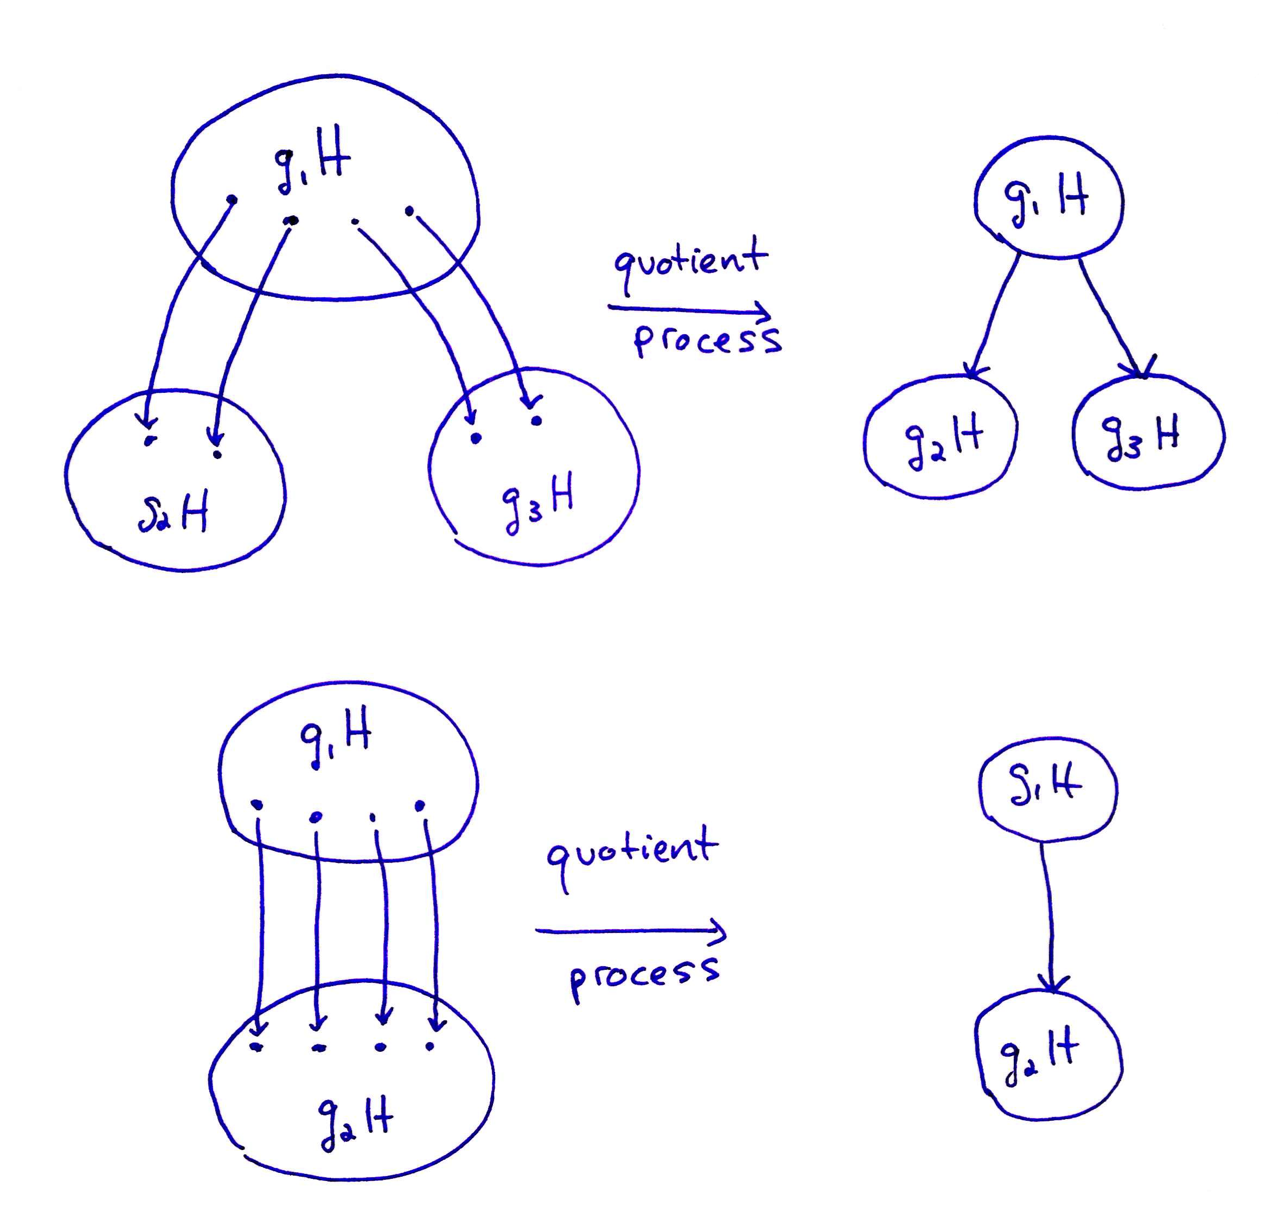
\includegraphics[width=5in]{QuotientProcess.png}
\caption{The quotient process.}
\label{fig:quotient_process}
\end{figure}

\begin{exercise}
In Exercise~\ref{exer:normal_in_D3}, we learned that the subgroup $K=\langle r\rangle$ is normal in $D_3$ since the left cosets are equal to the right cosets.  Note that this follows immediately from Theorem~\ref{thm:index2} since $[D_3:K]=2$.  Draw the diagram that results from performing the quotient process to $D_3$ using the subgroup $K$.  Does the resulting diagram represent a group?  If so, what group is it isomorphic to?
\end{exercise}

Now, suppose $G$ is an arbitrary group and let $H\leq G$. Consider the set of left cosets of $H$.  We define
\[
(aH)(bH):=(ab)H.
\]
The natural question to ask is whether this operation is well-defined.  That is, does the result of multiplying two left cosets depend on our choice of representatives?  More specifically, suppose $c\in aH$ and $d\in bH$.  Then $cH=aH$ and $dH=bH$.  According to the operation defined above, $(cH)(dH)=cdH$.  It better be the case that $cdH=abH$, otherwise the operation is not well-defined.

\begin{exercise}
Let $H=\langle s\rangle \leq D_3$.  Find specific examples of $a,b,c,d\in D_3$ such that $(aH)(bH)\neq (cH)(dH)$.
\end{exercise}

\begin{theorem}
Let $G$ be a group and let $H\leq G$.  Then left coset multiplication (as defined above) is well-defined if and only if $H\trianglelefteq G$.
\end{theorem}

\begin{theorem}\label{thm:quotient_grp}
Let $G$ be a group and let $H\trianglelefteq G$.  Then the set of left cosets of $H$ in $G$ forms a group under left coset multiplication.
\end{theorem}

The group from Theorem~\ref{thm:quotient_grp} is denoted by $G/H$, read ``$G$ mod $H$", and is referred to the \textbf{quotient group} (or \textbf{factor group}) of $G$ by $H$.  If $G$ is a finite group, then $G/H$ is exactly the group that arises from ``gluing together" the colored blocks in a checkerboard-patterned group table.  It's also the group that we get after applying the quotient process to the Cayley diagram.  It's important to point out once more that this only works properly if $H$ is a normal subgroup.

\begin{theorem}
Let $G$ be a group and let $H\trianglelefteq G$.  Then $|G/H|=[G:H]$.  In particular, if $G$ is finite, then $|G/H|=|G|/|H|$.
\end{theorem}

\begin{exercise}%Borrowing from Fraleigh Exercises 9--15 in Section 14.
Find the order of the given element in the quotient group. You may assume that we are taking the quotient by a normal subgroup. 
\begin{enumerate}
\item[(a)] $s\langle r\rangle \in D_4/\langle r\rangle$
\item[(b)] $j\langle -1\rangle \in Q_8/\langle -1\rangle$
\item[(c)] $5+\langle 4\rangle \in \mathbb{Z}_{12}/\langle 4\rangle$
\item[(d)] $(2,1)+\langle (1,1)\rangle \in (\mathbb{Z}_3\times \mathbb{Z}_6)/\langle (1,1)\rangle$ 
\end{enumerate}
 
\end{exercise}


\begin{exercise}
For each quotient group below, describe the group.  If possible, state what group each is isomorphic to.  You may assume that we are taking the quotient by a normal subgroup. 
\begin{enumerate}
\item[(a)] $Q_8/\langle -1\rangle$
\item[(b)] $Q_8/\langle i\rangle$
\item[(c)] $\mathbb{Z}_4/\langle 2\rangle$
\item[(d)] $V_4/\langle h\rangle$
\item[(e)] $A_4/\langle (1,2)(3,4),(1,3)(2,4)\rangle$
\item[(f)] $(\mathbb{Z}_2\times \mathbb{Z}_2)/\langle (1,1)\rangle$
\item[(g)] $\mathbb{Z}/4\mathbb{Z}$
\item[(h)] $S_4/A_4$
\item[(i)] $(\mathbb{Z}_4\times \mathbb{Z}_2)/(\{0\}\times \mathbb{Z}_2)$
\end{enumerate}
\end{exercise}

\begin{theorem}
Let $G$ be a group.  Then
\begin{enumerate}
\item $G/\{e\}\cong G$
\item $G/G\cong \{e\}$
\end{enumerate}
\end{theorem}

\begin{theorem}
For all $n\in \mathbb{N}$, we have the following.
\begin{enumerate}
\item $S_n/A_n\cong \mathbb{Z}_2$ (for $n\geq 3$)
\item $\mathbb{Z}/n\mathbb{Z}\cong \mathbb{Z}_n$
\item $\mathbb{R}/n\mathbb{R}\cong \{e\}$
\end{enumerate}
\end{theorem}

\begin{theorem}
Let $G$ be a group and let $H\trianglelefteq G$.  If $G$ is abelian, then so is $G/H$.
\end{theorem}

\begin{problem}
Show that the converse of the previous theorem is not true by providing a specific counterexample.
\end{problem}

\begin{exercise}
Consider the quotient group $(\mathbb{Z}_4\times \mathbb{Z}_6)/\langle (0,1)\rangle$.
\begin{enumerate}
\item[(a)] What is the order of $(\mathbb{Z}_4\times \mathbb{Z}_6)/\langle (0,1)\rangle$?
\item[(b)] Is the group abelian?  Why?
\item[(c)] Write down all the elements of $(\mathbb{Z}_4\times \mathbb{Z}_6)/\langle (0,1)\rangle$.
\item[(d)] Does one of the elements generate the group?
\item[(e)] What well-known group is $(\mathbb{Z}_4\times \mathbb{Z}_6)/\langle (0,1)\rangle$ isomorphic to?
\end{enumerate}
\end{exercise}

\begin{theorem}
Let $G$ be a group and let $H\trianglelefteq G$.  If $G$ is cyclic, then so is $G/H$.
\end{theorem}

\begin{problem}
Show that the converse of the previous theorem is not true by providing a specific counterexample.
\end{problem}

Here are few additional exercises.  These ones are a bit tougher.

\begin{exercise}
For each quotient group below, describe the group.  If possible, state what group each is isomorphic to.  You may assume that we are taking the quotient by a normal subgroup. 
\begin{enumerate}
\item[(a)] $(\mathbb{Z}_4\times \mathbb{Z}_6)/\langle (0,2)\rangle$
\item[(b)] $(\mathbb{Z}\times \mathbb{Z})/\langle (1,1)\rangle$
\item[(c)] $\mathbb{Q}/\langle 1\rangle$ (the operation on $\mathbb{Q}$ is addition)
\end{enumerate}
\end{exercise}

\end{section}
\chapter{Homomorphisms and the Isomorphism Theorems}
\label{chapter:homomorphisms}

\begin{section}{Homomorphisms}
Let $G_1$ and $G_2$ be groups. Recall that $\phi:G_1\to G_2$ is an isomorphism if and only if $\phi$
\begin{enumerate}[label=\textrm{(\alph*)}]
\item is one-to-one, 
\item is onto, and
\item satisfies the homomorphic property.
\end{enumerate}
We say that $G_1$ is isomorphic to $G_2$ and write $G_1\cong G_2$ if such a $\phi$ exists. Loosely speaking, two groups are isomorphic if they have the ``same structure."  What if we drop the one-to-one and onto requirement?

\begin{definition}
Let $(G_1,*)$ and $(G_2,\odot)$ be groups. A function $\phi:G_1\to G_2$ is a \textbf{homomorphism} if and only if $\phi$ satisfies the homomorphic property:
\[
\phi(x*y)=\phi(x)\odot\phi(y)
\]
for all $x,y\in G_1$. At the risk of introducing ambiguity, we will usually omit making explicit reference to the binary operations and write the homomorphic property as
\[
\phi(xy)=\phi(x)\phi(y).
\]
\end{definition}

Group homomorphisms are analogous to linear transformations on vector spaces that one encounters in linear algebra.

Figure~\ref{fig:isoGroupTables2} captures a visual representation of the homomorphic property.  We encountered this same representation in Figure~\ref{fig:isoGroupTables}. If $\phi(x)=x'$, $\phi(y)=y'$, and $\phi(z)=z'$ while $z'=x'\odot y'$, then the only way $G_2$ may respect the structure of $G_1$ is for
\[
\phi(x*y)=\phi(z)=z'=x'\odot y'=\phi(x)\odot \phi(y).
\]

\begin{figure}
\begin{center}
\begin{tabular}{c!{\vrule width 2pt}ccc|c|c}
$*$                & & & & \cellcolor{green}$y$  & \\ \noalign{\hrule height 2pt}
                   & & & &                       & \\ \hline
\cellcolor{red}$x$ & & & & \cellcolor{orange}$z$ & \\ \hline
                   & & & &                      & \\
                   & & & &                      &
\end{tabular}
\hspace{1cm}
$\longrightarrow$
\hspace{1cm}
\begin{tabular}{c!{\vrule width 2pt}ccc|c|c}
$\odot$                & & & & \cellcolor{green}$y'$  & \\ \noalign{\hrule height 2pt}
                   & & & &                       & \\ \hline
\cellcolor{red}$x'$ & & & & \cellcolor{orange}$z'$ & \\ \hline
                   & & & &                      & \\
                   & & & &                      &
\end{tabular}
\end{center}
\caption{}\label{fig:isoGroupTables2}
\end{figure}

\begin{problem}\label{prob:homomorphism}
Define $\phi:\mathbb{Z}_3\to D_3$ via $\phi(k)=r^k$. Prove that $\phi$ is a homomorphism and then determine whether $\phi$ is one-to-one or onto. Also, try to draw a picture of the homomorphism in terms of Cayley diagrams.
\end{problem}

\begin{problem}
Let $G$ and $H$ be groups. Prove that the function $\phi:G\times H\to G$ given by $\phi(g,h)=g$ is a homomorphism. This function is an example of a \textbf{projection map}.
\end{problem}

There is always at least one homomorphism between two groups.

\begin{theorem}\label{thm:trivial_homomorphism}
Let $G_1$ and $G_2$ be groups. Define $\phi:G_1\to G_2$ via $\phi(g)=e_2$ (where $e_2$ is the identity of $G_2$).  Then $\phi$ is a homomorphism. This function is often referred to as the \textbf{trivial homomorphism} or the \textbf{$0$-map}.
\end{theorem}

Back in Section~\ref{sec:isomorphisms}, we encountered several theorems about isomorphisms.  However, at the end of that section we remarked that some of those theorems did not require that the function be one-to-one and onto.  We collect those results here for convenience.

\begin{theorem}
Let $G_1$ and $G_2$ be groups and suppose $\phi:G_1\to G_2$ is a homomorphism.
\begin{enumerate}[label=\textrm{(\alph*)}]
\item If $e_1$ and $e_2$ are the identity elements of $G_1$ and $G_2$, respectively, then $\phi(e_1)=e_2$.
\item For all $g\in G_1$, we have $\phi(g^{-1})=[\phi(g)]^{-1}$.
\item If $H\leq G_1$, then $\phi(H)\leq G_2$, where
\[
\phi(H):=\{y\in G_2\mid \text{there exists } h\in H\text{ such that }\phi(h)=y\}. 
\]
Note that $\phi(H)$ is called the \textbf{image} of $H$. A special case is when $H=G_1$. Notice that $\phi$ is onto exactly when $\phi(G_1)=G_2$.
\end{enumerate}
\end{theorem}

The following theorem is a consequence of Lagrange's Theorem.

\begin{theorem}
Let $G_1$ and $G_2$ be groups such that $G_2$ is finite and let $H\leq G_1$. If $\phi:G_1\to G_2$ is a homomorphism, then $|\phi(H)|$ divides $|G_2|$.
\end{theorem}

The next theorem tells us that under a homomorphism, the order of the image of an element must divide the order of the pre-image of that element.

\begin{theorem}\label{thm:orderImage}
Let $G_1$ and $G_2$ be groups and suppose $\phi:G_1\to G_2$ is a homomorphism. If $g\in G_1$ such that $|g|$ is finite, then $|\phi(g)|$ divides $|g|$.
\end{theorem}

Every homomorphism has an important subset of the domain associated with it.

\begin{definition}
Let $G_1$ and $G_2$ be groups and suppose $\phi:G_1\to G_2$ is a homomorphism.  The \textbf{kernel} of $\phi$ is defined via
\[
\ker(\phi):=\{g\in G_1\mid \phi(g)=e_2\}.
\]
\end{definition}

The kernel of a homomorphism is analogous to the null space of a linear transformation of vector spaces.  

\begin{problem}
Identify the kernel and image for the homomorphism given in Problem~\ref{prob:homomorphism}.
\end{problem}

\begin{problem}
What is the kernel of a trivial homomorphism (see Theorem~\ref{thm:trivial_homomorphism}).
\end{problem}

\begin{theorem}\label{thm:kernel_normal}
Let $G_1$ and $G_2$ be groups and suppose $\phi:G_1\to G_2$ is a homomorphism. Then $\ker(\phi)\trianglelefteq G_1$.
\end{theorem}

\begin{theorem}\label{thm:canonical_projection}
Let $G$ be a group and let $H\trianglelefteq G$.  Then the map $\gamma:G\to G/H$ given by $\gamma(g)=gH$ is a homomorphism with $\ker(\gamma)=H$. This map is called the \textbf{canonical projection map}.
\end{theorem}

The upshot of Theorems~\ref{thm:kernel_normal} and \ref{thm:canonical_projection} is that kernels of homomorphisms are always normal and every normal subgroup is the kernel of some homomorphism. It turns out that the kernel can tell us whether $\phi$ is one-to-one.

The next theorem tells us that two elements in the domain of a group homomorphism map to the same element in the codomain if and only if they are in the same coset of the kernel.

\begin{theorem}\label{thm:same_image}
Let $G_1$ and $G_2$ be groups and suppose $\phi:G_1\to G_2$ is a homomorphism. Then $\phi(a) = \phi(b)$ if and only if $a\in b\ker(\phi)$.
\end{theorem}

One consequence of Theorem~\ref{thm:same_image} is that if the kernel of a homomorphism has order $k$, then the homomorphism is $k$-to-1.  That is, every element in the range has exactly $k$ elements from the domain that map to it.  In particular, each of these collections of $k$ elements corresponds to a coset of the kernel. 

\begin{problem}
Suppose $\phi:\mathbb{Z}_{20}\to\mathbb{Z}_{20}$ is a group homomorphism such that $\ker(\phi)=\{0,5,10,15\}$.  If $\phi(13)=8$, determine all elements that $\phi$ maps to 8.
\end{problem}

The next result is a special case of Theorem~\ref{thm:same_image}.

\begin{theorem}\label{thm:trivial_kernel}
Let $G_1$ and $G_2$ be groups and suppose $\phi:G_1\to G_2$ is a homomorphism. Then $\phi$ is one-to-one if and only if $\ker(\phi)=\{e_1\}$, where $e_1$ is the identity in $G_1$.
\end{theorem}

Let $G_1$ and $G_2$ be groups and suppose $\phi:G_1\to G_2$ is a homomorphism. Given a generating set for $G_1$, the homomorphism $\phi$ is uniquely determined by its action on the generating set for $G_1$.  In particular, if you have a word for a group element written in terms of the generators, just apply the homomorphic property to the word to find the image of the corresponding group element.

\begin{problem}\label{prob:Q8toV4}
Suppose $\phi: Q_8\to V_{4}$ is a group homomorphism satisfying $\phi(i)=h$ and $\phi(j)=v$.
\begin{enumerate}[label=\textrm{(\alph*)}]
\item Find $\phi(1)$, $\phi(-1)$, $\phi(k)$, $\phi(-i)$, $\phi(-j)$, and $\phi(-k)$.
\item Find $\ker(\phi)$.
\item What well-known group is $Q_8/\ker(\phi)$ isomorphic to?
\end{enumerate}
\end{problem}

\begin{problem}
Find a non-trivial homomorphism from $\mathbb{Z}_{10}$ to $\mathbb{Z}_6$.
\end{problem}

\begin{problem}
Find all non-trivial homomorphisms from $\mathbb{Z}_3$ to $\mathbb{Z}_6$.
\end{problem}

\begin{problem}
Prove that the only homomorphism from $D_3$ to $\mathbb{Z}_3$ is the trivial homomorphism.
\end{problem}

\begin{problem}
Let $F$ be the set of all functions from $\mathbb{R}$ to $\mathbb{R}$ and let $D$ be the subset of differentiable functions on $\mathbb{R}$.  It turns out that $F$ is a group under addition of functions and $D$ is a subgroup of $F$ (you do not need to prove this). Define $\phi:D\to F$ via $\phi(f)=f'$ (where $f'$ is the derivative of $f$). Prove that $\phi$ is a homomorphism.  You may recall facts from calculus without proving them. Is $\phi$ one-to-one? Onto? 
\end{problem}

\end{section}

\begin{section}{The Isomorphism Theorems}

The next theorem is arguably the crowning achievement of the course.

\begin{theorem}[The First Isomorphism Theorem]
Let $G_1$ and $G_2$ be groups and suppose $\phi:G_1\to G_2$ is a homomorphism. Then
\[
G_1/\ker(\phi)\cong \phi(G_1).
\]
If $\phi$ is onto, then
\[
G_1/\ker(\phi)\cong G_2.
\]
\end{theorem}

\begin{problem}
Let $\phi:Q_8\to V_4$ be the homomorphism described in Problem~\ref{prob:Q8toV4}. Use the First Isomorphism Theorem to prove that $Q_8/\langle-1\rangle\cong V_4$.
\end{problem}

\begin{problem}
For $n\geq 2$, define $\phi:S_n\to \mathbb{Z}_2$ via
\[
\phi(\sigma)=\begin{cases}
0, & \sigma \text{ even}\\
1, & \sigma \text{ odd}.
\end{cases}
\]
Use the First Isomorphism Theorem to prove that $S_n/A_n\cong \mathbb{Z}_2$.
\end{problem}

\begin{problem}
Use the First Isomorphism Theorem to prove that $\mathbb{Z}/6\mathbb{Z}\cong \mathbb{Z}_6$.  Attempt to draw a picture of this using Cayley diagrams.
\end{problem}

\begin{problem}
Use the First Isomorphism Theorem to prove that $(\mathbb{Z}_4\times \mathbb{Z}_2)/(\{0\}\times \mathbb{Z}_2)\cong \mathbb{Z}_4$.
\end{problem}

The next theorem is a generalization of Theorem~\ref{thm:orderImage} and follows from the First Isomorphism Theorem together with Lagrange's Theorem.

\begin{theorem}
Let $G_1$ and $G_2$ be groups and suppose $\phi:G_1\to G_2$ is a homomorphism. If $G_1$ is finite, then $|\phi(G_1)|$ divides $|G_1|$.
\end{theorem}

We finish the chapter by listing a few of the remaining isomorphism theorems.%, but we will not prove these in this course.

\begin{theorem}[The Second Isomorphism Theorem]
Let $G$ be a group with $H\leq G$ and $N\trianglelefteq G$.  Then
\begin{enumerate}[label=\textrm{(\alph*)}]
\item $HN:=\{hn\mid h\in H, n\in N\}\leq G$;
\item $H\cap N\trianglelefteq H$;
\item $\displaystyle H/(H\cap N)\cong HN/N$.
\end{enumerate}
\end{theorem}

\begin{theorem}[The Third Isomorphism Theorem]
Let $G$ be a group with $H,K\trianglelefteq G$ and $K\leq H$.  Then $H/K\trianglelefteq G/K$ and
\[
G/H\cong (G/K)/(H/K).
\]
\end{theorem}

The last isomorphism theorem is sometimes called the \emph{Lattice Isomorphism Theorem} or the \emph{Correspondence Theorem}.

\begin{theorem}[The Fourth Isomorphism Theorem]

Let $G$ be a group with $N\trianglelefteq G$. Then there is a bijection from the set of subgroups of $G$ that contain $N$ onto the set of subgroups of $G/N$. In particular, every subgroup $G$ is of the form $H/N$ for some subgroup $H$ of $G$ containing $N$ (namely, its preimage in $G$ under the canonical projection homomorphism from $G$ to $G/N$.) This bijection has the following properties: for all $H,K \leq G$ with  $N\leq H$ and $N\subseteq K$, we have
\begin{enumerate}[label=\textrm{(\alph*)}]
\item $H\leq K$ if and only if $H/N \leq K/N$
\item If $H\leq K$, then $|K:H|=|K/N:H/N|$
\item $\langle H,K\rangle/N=\langle H/N,K/N\rangle$
\item $(H\cap K)/N=H/N \cap K/N$
\item $H\trianglelefteq G$ if and only if $H/N\trianglelefteq G/N$.
\end{enumerate}
\end{theorem}

\end{section}
\chapter{An Introduction to Rings}
\label{chapter:rings}
\thispagestyle{empty}

\begin{section}{Definitions and Examples}

Recall that a group is a set together with a single binary operation, which together satisfy a few modest properties. Loosely speaking, a ring is a set together with two binary operations (called addition and multiplication) that are related via a distributive property.

\begin{definition}
A \textbf{ring} $R$ is a set together with two binary operations $+$ and $\cdot$ (called \textbf{addition} and \textbf{multiplication}, respectively) satisfying the following:
\begin{enumerate}
\item[(i)] $(R,+)$ is an abelian group.
\item[(ii)] $\cdot$ is associative: $(a\cdot b)\cdot c=a\cdot (b\cdot c)$ for all $a,b,c\in R$.
\item[(iii)] The \textbf{distributive property} holds: $a\cdot (b+c)=(a\cdot b)+(a\cdot c)$ and $(a+b)\cdot c = (a\cdot c)+(b\cdot c)$ for all $a,b,c\in R$.
\end{enumerate}
\end{definition}

\begin{remark}
We make a couple comments about notation.
\begin{enumerate}[label=\rm{(\alph*)}]
\item We often write $ab$ in place $a\cdot b$.
\item The additive inverse of the ring element $a\in R$ is denoted $-a$.
\end{enumerate}
\end{remark}

\begin{theorem}
Let $R$ be a ring.  Then for all $a,b\in R$:
\begin{enumerate}
\item $0a=a0=0$
\item $(-a)b=a(-b)=-(ab)$
\item $(-a)(-b)=ab$
\end{enumerate}
\end{theorem}

\begin{definition}
A ring $R$ is called \textbf{commutative} if multiplication is commutative.
\end{definition}

\begin{definition}
A ring $R$ is said to have an \textbf{identity} (or called a \textbf{ring with  1}) if there is an element $1\in R$ such that $1a=a 1=a$ for all $a\in R$.
\end{definition}

\begin{exercise}
Justify that $\mathbb{Z}$ is a commutative ring with 1 under the usual operations of addition and multiplication. Which elements have multiplicative inverses in $\mathbb{Z}$?
\end{exercise}

\begin{exercise}
Justify that $\mathbb{Z}_n$ is a commutative ring with 1 under addition and multiplication mod $n$.
\end{exercise}

\begin{exercise}\label{exer:Z10Ring}
Consider the set $\mathbb{Z}_{10}=\{0,1,2,3,4,5,6,7,8,9\}$. Which elements have multiplicative inverses in $\mathbb{Z}_{10}$?
\end{exercise}

\begin{exercise}
For each of the following, find a positive integer $n$ such that the ring $\mathbb{Z}_n$ does not have the stated property.
\begin{enumerate}[label=\rm{(\alph*)}]
\item $a^2=a$ implies $a=0$ or $a=1$.
\item $ab=0$ implies $a=0$ or $b=0$.
\item $ab=ac$ and $a\neq 0$ imply $b=c$.
\end{enumerate}
\end{exercise}

\begin{theorem}
If $R$ is a ring with 1, then the multiplicative identity is unique and $-a=(-1)a$.
\end{theorem}

\begin{problem}
Requiring $(R,+)$ to be a group is fairly natural, but why require $(R,+)$ to be abelian?  Suppose $R$ has a 1.  Compute $(1+1)(a+b)$ in two different ways.
\end{problem}

\begin{definition}
A ring $R$ with 1 (with $1\neq 0$) is called a \textbf{division ring} if every nonzero element in $R$ has a multiplicative inverse: if $a\in R\setminus\{0\}$, then there exists $b\in R$ such that $ab=ba=1$.
\end{definition}

\begin{definition}
A commutative division ring is called a \textbf{field}.
\end{definition}

\begin{definition}
A nonzero element $a$ in a ring $R$ is called a \textbf{zero divisor} if there is a nonzero element $b\in R$ such that either $ab=0$ or $ba=0$.
\end{definition}

\begin{exercise}
Are there any zero divisors in $\mathbb{Z}_{10}$?  If so, find all of them.
\end{exercise}

\begin{exercise}
Are there any zero divisors in $\mathbb{Z}_5$?  If so, find all of them.
\end{exercise}

\begin{exercise}
Provide an example of a ring $R$ and elements $a,b\in R$ such that $ax=b$ has more than one solution.  How does this compare with groups?
\end{exercise}

\begin{theorem}[Cancellation Law]\label{thm:RingCancellation}
Assume $a,b,c\in R$ such that $a$ is not a zero divisor.  If $ab=ac$, then either $a=0$ or $b=c$.
\end{theorem}

\begin{definition}
Assume $R$ is a ring with $1$ with $1\neq 0$. An element $u\in R$ is called a \textbf{unit} in $R$ if $u$ has a multiplicative inverse (i.e., there exists $v\in R$ such that $uv=vu=1$.  The set of units in $R$ is denoted $U(R)$.
\end{definition}

\begin{exercise}
Consider the ring $\mathbb{Z}_{20}$.
\begin{enumerate}[label=\rm{(\alph*)}]
\item Find $U(\mathbb{Z}_{20})$.
\item Find the zero divisors of $\mathbb{Z}_{20}$.
\item Any observations?
\end{enumerate}
\end{exercise}

\begin{theorem}
If $U(R)\neq\emptyset$, then $U(R)$ forms a group under multiplication.
\end{theorem}

\begin{remark}
We make a few observations.
\begin{enumerate}[label=\rm{(\alph*)}]
\item A field is a commutative ring $F$ with identity $1\neq 0$ in which every nonzero element is a unit, i.e., $U(F)=F\setminus\{0\}$.
\item Zero divisors can never be units.
\item Fields never have zero divisors.
\end{enumerate}
\end{remark}

\begin{definition}
A commutative ring with identity $1\neq 0$ is called an \textbf{integral domain} if it has no zero divisors.
\end{definition}

\begin{remark}
The Cancellation Law (Theorem~\ref{thm:RingCancellation}) holds in integral domains for any three elements.
\end{remark}

\begin{corollary}
Any finite integral domain is a field.
\end{corollary}

%\begin{proof}
%For any nonzero $a\in R$, define $f_a:R\to R$ via $f_a(x)=ax$.  If $R$ is an integral domain, the Cancellation Law forces $f_a$ to be injective.  If $R$ is finite, then $f_a$ is also surjective.  In this case, there exists $b\in R$ such that $ab=1$.
%\end{proof}

\begin{example}
Here are a few examples.  Details left as an exercise.
\begin{enumerate}[label=\rm{(\alph*)}]
\item \textbf{Zero Ring}: If $R=\{0\}$, we can turn $R$ into a ring in the obvious way.  The zero ring is a finite commutative ring with 1.  It is the only ring where the additive and multiplicative identities are equal.  The zero ring is not a division ring, not a field, and not an integral domain.
\item \textbf{Trivial Ring:} Given any abelian group $R$, we can turn $R$ into a ring by defining multiplication via $ab=0$ for all $a,b\in R$. Trivial rings are commutative rings in which every nonzero element is a zero divisor.  Hence a trivial ring is not a division ring, not a field, and not a integral domain.
\item 
%The integers $\mathbb{Z}$ form a ring under the usual operations of addition and multiplication.  
The integers form an integral domain, but $\mathbb{Z}$ is not a division ring, and hence not a field.
\item The rational numbers $\mathbb{Q}$, the real numbers $\mathbb{R}$, and the complex numbers $\mathbb{C}$ are fields under the usual operations of addition and multiplication.
\item 
%For $n\geq 1$, the set $\mathbb{Z}_n$ is a commutative ring with 1 under the operations of addition and multiplication mod $n$. 
The group of units $U(\mathbb{Z}_n)$ is the set of elements in $\mathbb{Z}_n$ that are relatively prime to $n$.  All other nonzero elements are zero divisors.  It turns out that $\mathbb{Z}_n$ forms a finite field iff $n$ is prime.
\item The set of even integers $2\mathbb{Z}$ forms a commutative ring under the usual operations of addition and multiplication.  However, $2\mathbb{Z}$ does not have a 1, and hence cannot be a division ring nor a field nor an integral domain.
\item \textbf{Polynomial Ring:} Fix a commutative ring $R$.  Let $R[x]$ denote the set of polynomials in the variable $x$ with coefficients in $R$.  Then $R[x]$ is a commutative ring with 1. The units of $R[x]$ are exactly the units of $R$ (if there are any). So, $R[x]$ is never a division ring nor a field.  However, if $R$ is an integral domain, then so is $R[x]$. 
\item \textbf{Matrix Ring:} Fix a ring $R$ and let $n$ be a positive integer.  Let $M_n(R)$ be the set of $n\times n$ matrices with entries from $R$.  Then $M_n(R)$ forms a ring under ordinary matrix addition and multiplication.  If $R$ is nontrivial and $n\geq 2$, then $M_n(R)$ always has zero divisors and $M_n(R)$ is not commutative even if $R$ is.  If $R$ has a 1, then the matrix with 1's down the diagonal and 0's elsewhere is the multiplicative identity in $M_n(R)$.  In this case, the group of units is the set of invertible $n\times n$ matrices, denoted $GL_n(R)$ and called the \textbf{general linear group of degree $n$ over $R$}.
\item \textbf{Quadratic Field:} Define $\mathbb{Q}(\sqrt{2})=\{a+b\sqrt{2}\mid a,b\in\mathbb{Q}\}$.  It turns out that $\mathbb{Q}(\sqrt{2})$ is a field.  In fact, we can replace 2 with any rational number that is not a perfect square in $\mathbb{Q}$.
\item \textbf{Hamilton Quaternions:} Define $\mathbb{H}=\{a+bi+cj+dk\mid a,b,c,d\in\mathbb{R}, i,j,k\in Q_8\}$  Then $\mathbb{H}$ forms a ring, where addition is definite componentwise in $i$, $j$, and $k$ and multiplication is defined by expanding products and the simplifying using the relations of $Q_8$.  It turns out that $\mathbb{H}$ is a non-commutative ring with 1.
\end{enumerate}
\end{example}

\begin{exercise}
Find an example of a ring $R$ and an element $a\in R\setminus\{0\}$ such that $a$ is neither a zero divisor nor a unit.
\end{exercise}

\begin{definition}
A \textbf{subring} of a ring $R$ is a subgroup of $R$ that is closed under multiplication.
\end{definition}

\begin{remark}
The property ``is a subring" is clearly transitive. To show that a subset $S$ of a ring $R$ is a subring, it suffices to show that $S\neq \emptyset$, $S$ is closed under subtraction, and $S$ is closed under multiplication.
\end{remark}

\begin{example}
Here are a few quick examples.
\begin{enumerate}[label=\rm{(\alph*)}]
\item $\mathbb{Z}$ is a subring of $\mathbb{Q}$, which is a subring of $\mathbb{R}$, which in turn is a subring of $\mathbb{C}$.
\item $2\mathbb{Z}$ is a subring of $\mathbb{Z}$.
\item The set $\mathbb{Z}(\sqrt{2})=\{a+b\sqrt{2}\mid a,b\in\mathbb{Z}\}$ is a subring of $\mathbb{Q}(\sqrt{2})$.
\item The ring $R$ is a subring of $R[x]$ if we identify $R$ with set of constant functions.
\item The set of polynomials with zero constant term in $R[x]$ is a subring of $R[x]$.
\item $\mathbb{Z}[x]$ is a subring of $\mathbb{Q}[x]$.
\item $\mathbb{Z}_n$ is \emph{not} a subring of $\mathbb{Z}$ as the operations are different.
\end{enumerate} 
\end{example}

\begin{problem}
Consider the ring $\mathbb{Z}_{10}$ from Exercise~\ref{exer:Z10Ring}. Let $S=\{0,2,4,6,8\}$.
\begin{enumerate}[label=\rm{(\alph*)}]
\item Argue that $S$ is a subring of $R$.
\item Is $S$ a ring with 1?  If so, find the multiplicative identity.  If not, explain why.
\item Is $S$ a field? Justify your answer.
\end{enumerate}
\end{problem}

\begin{problem}
Suppose $R$ is a ring and let $a\in R$.  Define $S=\{x\in R\mid ax=0\}$.  Prove that $S$ is a subring of $R$.
\end{problem}

\begin{problem}
Consider the ring $\mathbb{Z}$.  It turns out that $2\mathbb{Z}$ and $3\mathbb{Z}$ are subrings (but you don't need to prove this).  Determine whether $2\mathbb{Z}\cup 3\mathbb{Z}$ is a subring of $\mathbb{Z}$.  Justify your answer.
\end{problem}

\end{section}

\begin{section}{Ring Homomorphisms}

\begin{definition}
Let $R$ and $S$ be rings.  A \textbf{ring homomorphism} is a map $\phi:R\to S$ satisfying
\begin{enumerate}[label=\rm{(\alph*)}]
\item[(i)] $\phi(a+b)=\phi(a)+\phi(b)$
\item[(ii)] $\phi(ab)=\phi(a)\phi(b)$
\end{enumerate}
for all $a,b\in R$. The \textbf{kernel} of $\phi$ is defined via $\ker(\phi)=\{a\in R\mid \phi(a)=0\}$.  If $\phi$ is a bijection, then $\phi$ is called an \textbf{isomorphism}, in which case, we say that $R$ and $S$ are \textbf{isomorphic rings} and write $R\cong S$.
\end{definition}

\begin{example}
\ 
\begin{enumerate}[label=\rm{(\alph*)}]
\item For $n\in \mathbb{Z}$, define $\phi_n:\mathbb{Z}\to \mathbb{Z}$ via $\phi_n(x)=nx$.  We see that $\phi_n(x+y)=n(x+y)=nx+ny=\phi_n(x)+\phi_n(y)$.  However, $\phi_n(xy)=n(xy)$ while $\phi_n(x)\phi_n(y)=(nx)(ny)=n^2xy$.  It follows that $\phi_n$ is a ring homomorphism exactly when $n\in\{0,1\}$.
\item Define $\phi:\mathbb{Q}[x]\to \mathbb{Q}$ via $\phi(p(x))=p(0)$ (called \textbf{evaluation at 0}).  It turns out that $\phi$ is a ring homomorphism, where $\ker(\phi)$ is the set of polynomials with 0 constant term.
\end{enumerate}
\end{example}

\begin{exercise}
For each of the following, determine whether the given function is a ring homomorphism.  Justify your answers.
\begin{enumerate}[label=\rm{(\alph*)}]
\item Define $\phi:\mathbb{Z}_4\to \mathbb{Z}_{12}$ via $\phi(x)=3x$.
\item Define $\phi:\mathbb{Z}_{10}\to \mathbb{Z}_{10}$ via $\phi(x)=5x$.
\item Let $\displaystyle S=\left\{\begin{pmatrix}a & b\\ -b & a\end{pmatrix}\mid a, b\in \mathbb{R}\right\}$.  Define $\phi:\mathbb{C}\to S$ via $\displaystyle \phi(a+ib)=\begin{pmatrix}a & b\\ -b & a\end{pmatrix}$.
\item Let $\displaystyle T=\left\{\begin{pmatrix}a & b\\ 0 & c\end{pmatrix}\mid a, b\in \mathbb{Z}\right\}$. Define $\phi:T\to \mathbb{Z}$ via $\displaystyle \phi\left(\begin{pmatrix}a & b\\ 0 & c\end{pmatrix}\right)=a$.
\end{enumerate}
\end{exercise}

\begin{problem}
Suppose $\phi:R\to S$ is a ring homomorphism such that $R$ is a ring with 1, call it $1_R$.  Prove that $\phi(1_R)$ is the multiplicative identity in $\phi(R)$ (which is a subring of $S$).  Can you think of an example of a ring homomorphism where $S$ has a multiplicative identity that is not equal to $\phi(1_R)$?
\end{problem}

\begin{theorem}
Let $\phi:R\to S$ be a ring homomorphism.
\begin{enumerate}
\item $\phi(R)$ is a subring of $S$.
\item $\ker(\phi)$ is a subring of $R$.
\end{enumerate}
\end{theorem}

In fact, we can say something even stronger about the kernel of a ring homomorphism, which will lead us to the notion of an \textbf{ideal}.

\begin{theorem}
Let $\phi:R\to S$ be a ring homomorphism.  If $\alpha\in\ker(\phi)$ and $r\in R$, then $\alpha r, r\alpha\in \ker(\phi)$.  That is, $\ker(\phi)$ is closed under multiplication by elements of $R$.
\end{theorem}

\end{section}

\begin{section}{Ideals and Quotient Rings}

Recall that in the case of a homomorphism $\phi$ of groups, the cosets of $\ker(\phi)$ have the structure of a group (that happens to be isomorphic to the image of $\phi$ by the First Isomorphism Theorem).  In this case, $\ker(\phi)$ is the identity of the associated quotient group.  Moreover, recall that every kernel is a normal subgroup of the domain and every normal subgroup can be realized as the kernel of some group homomorphism.  Can we do the same sort of thing for rings?

Let $\phi:R\to S$ be a ring homomorphism with $\ker(\phi)=I$.  Note that $\phi$ is also a group homomorphism of abelian groups and the cosets of $\ker(\phi)$ are of the form $r+I$.  More specifically, if $\phi(r)=a$, then $\phi^{-1}(a)=r+I$.

These cosets naturally have the structure of a ring isomorphic to the image of $\phi$:
\begin{align}
(r+I)+(s+I) & =  (r+s)+I\\
(r+I)(s+I) & = (rs)+I
\end{align}
The reason for this is that if $\phi^{-1}(a)=X$ and $\phi^{-1}(b)=Y$, then the inverse image of $a+b$ and $ab$ are $X+Y$ and $XY$, respectively.

The corresponding ring of cosets is called the \textbf{quotient ring} of $R$ by $I=\ker(\phi)$ and is denoted by $R/I$.  The additive structure of the quotient ring $R/I$ is exactly the additive quotient group of the additive abelian group $R$ by the normal subgroup $R$ (all subgroups are normal in abelian groups).  When $I$ is the kernel of some ring homomorphism $\phi$, the additive abelian quotient group $R/I$ also has a multiplicative structure defined in (2) above, making $R/I$ into a ring.

\begin{center}
\emph{Can we make $R/I$ into a ring for any subring $I$?}
\end{center}

The answer is ``no" in general, just like in the situation with groups.  But perhaps this isn't obvious because if $I$ is an arbitrary subring of $R$, then $I$ is necessarily an additive subgroup of the abelian group $R$, which implies that $I$ is an additive normal subgroup of the group $R$.  It turns out that the multiplicative structure of $R/I$ may not be well-defined if $I$ is an arbitrary subring.

Let $I$ be an arbitrary \emph{subgroup} of the additive subgroup $R$.  Let $r+I$ and $s+I$ be two arbitrary cosets.  In order for multiplication of the cosets to be well-defined, the product of the two cosets must be independent of choice of representatives.  Let $r+\alpha$ and $s+\beta$ be arbitrary representatives of $r+I$ and $s+I$, respectively ($\alpha,\beta\in I$), so that $r+I=(r+\alpha)+I$ and $s+I=(s+\beta)+I$.  We must have
\begin{align}
(r+\alpha)(s+\beta)+I & =rs+I.
\end{align}
This needs to be true for all possible choices of $r,s\in R$ and $\alpha, \beta\in I$.  In particular, it must be true when $r=s=0$.  In this case, we must have
\begin{align}
\alpha\beta+I & =I.
\end{align}
But this only happens when $\alpha\beta\in I$.  That is, one requirement for multiplication of cosets to be well-defined is that $I$ must be closed under multiplication, making $I$ a \emph{subring}.

Next, if we let $s=0$ and let $r$ be arbitrary, we see that we must have $r\beta\in I$ for every $r\in R$ and every $\beta\in I$.  That is, it must be the case that $I$ is closed under multiplication on the left by elements from $R$.  Similarly, letting $r=0$, we can conclude that we must have $I$ closed under multiplication on the right by elements from $R$.  

On the other hand, if $I$ is closed under multiplication on the left and on the right by elements from $R$, then it is clear that relation (4) above is satisfied.

It is easy to verify that if the multiplication of cosets defined in (2) above is well-defined, then this multiplication makes the additive quotient group $R/I$ into a ring (just check the axioms for being a ring).

We have shown that the quotient $R/I$ of the ring $R$ by a subgroup $I$ has a natural ring structure iff $I$ is closed under multiplication on the left and right by elements of $R$ (which also forces $I$ to be a subring).  Such subrings are called \textbf{ideals}.

\begin{definition}
Let $R$ be a ring and let $I$ be a subset of $R$.
\begin{enumerate}[label=\rm{(\alph*)}]
\item $I$ is a \textbf{left ideal} (respectively, \textbf{right ideal}) of $R$ iff $I$ is a subring and $rI\subseteq I$ (respectively, $Ir\subseteq I$) for all $r\in R$.
\item $I$ is an \textbf{ideal} (or \textbf{two-sided ideal}) iff $I$ is both a left and a right ideal.
\end{enumerate}
\end{definition}

Here's a summary of everything that just happened.

\begin{theorem}
Let $R$ be a ring and let $I$ be an ideal of $R$.  Then the additive quotient group $R/I$ is a ring under the binary operations:
\begin{align}
(r+I)+(s+I) & =  (r+s)+I\\
(r+I)(s+I) & = (rs)+I
\end{align}
for all $r,s\in R$.  Conversely, if $I$ is any subgroup such that the above operations are well-defined, then $I$ is an ideal of $R$.
\end{theorem}

\begin{theorem}
Suppose $I$ and $J$ are ideals of the ring $R$.  Then $I\cap J$ is an ideal of $R$.
\end{theorem}

As you might expect, we have some isomorphism theorems.

\begin{theorem}[First Isomorphism Theorem for Rings]
If $\phi:R\to S$ is a ring homomorphism, then $\ker(\phi)$ is an ideal of $R$ and $R/\ker(\phi)\cong \phi(R)$.
\end{theorem}

%If $I$ and $J$ are ideals of $R$, then it is easy to verify that $I\cap J$, $I+J=\{a+b\mid a\in I, b\in J\}$, and $IJ=\{\text{finite sums of elements of the form }ab\text{ for }a\in I, b\in J\}$ are also ideals of $R$.

We also have the expected Second and Third Isomorphism Theorems for rings.  

The next theorem tells us that a subring is an ideal iff it is a kernel of a ring homomorphism.

\begin{theorem}
If $I$ is any ideal of $R$, then the \textbf{natural projection} $\pi:R\to R/I$ defined via $\pi(r)=r+I$ is a surjective ring homomorphism with $\ker(\pi)=I$.
\end{theorem}

For the remainder of this section, assume that $R$ is a ring with identity $1\neq 0$.

\begin{definition}
Let $A$ be any subset of $R$. Let $(A)$ denote the smallest ideal of $R$ containing $A$, called the \textbf{ideal generated by $A$}. If $A$ consists of a single element, say $A=\{a\}$, then $(a):=(\{a\})$ is called a \textbf{principal ideal}.
\end{definition}

\begin{remark}
The following facts are easily verified.
\begin{enumerate}[label=\rm{(\alph*)}]
\item $(A)$ is the intersection of all ideals containing $A$.
\item If $R$ is commutative, then $(a)=aR:=\{ar\mid r\in R\}$.
\end{enumerate}
\end{remark}

\begin{example}\label{ex:PrincipalIdeals}
In $\mathbb{Z}$, $n\mathbb{Z}=(n)=(-n)$.  In fact, these are the only ideals in $\mathbb{Z}$ (since these are the only subgroups). So, all the ideals in $\mathbb{Z}$ are principal. If $m$ and $n$ are positive integers, then $n\mathbb{Z}\subseteq m\mathbb{Z}$ iff $m$ divides $n$.  Moreover, we have $(m,n)=(d)$, where $d$ is the greatest common divisor of $m$ and $n$.
\end{example}

\begin{problem}
Consider the ideal $(2,x)$ in $\mathbb{Z}[x]$. Note that $(2,x)=\{2p(x)+xq(x)\mid p(x),q(x)\in\mathbb{Z}[x]\}$.  Argue that $(2,x)$ is not a principal ideal, i.e., there is no single polynomial in $\mathbb{Z}[x]$ that we can use to generate $(2,x)$.
\end{problem}

\begin{theorem}
Assume $R$ is a commutative ring with 1. Let $I$ be an ideal of $R$. Then $I=R$ iff $I$ contains a unit.
\end{theorem}

\begin{theorem}
Assume $R$ is a commutative ring with 1.  Then $R$ is a field iff its only ideals are $0$ and $R$.
\end{theorem}

Loosely speaking, the previous results say that fields are ``like simple groups" (i.e, groups with no non-trivial normal subgroups).

\begin{corollary}\label{cor:HomFromField}
If $R$ is a field, then every nonzero ring homomorphism from $R$ into another ring is an injection.
\end{corollary}

\end{section}

\begin{section}{Maximal and Prime Ideals}

Throughout this entire section, we assume that all rings have a multiplicative identity $1\neq 0$.

In this section of notes, we will study two important classes of ideals, namely \textbf{maximal} and \textbf{prime} ideals, and study the relationship between them. 

\begin{definition}
Assume $R$ is a commutative ring with 1. An ideal $M$ in a ring $R$ is called a \textbf{maximal ideal} if $M\neq R$ and the only ideals containing $M$ are $M$ and $R$.
\end{definition}

\begin{example}
Here are a few examples.  Checking the details is left as an exercise.
\begin{enumerate}[label=\rm{(\arabic*)}]
\item In $\mathbb{Z}$, all the ideals are of the form $n\mathbb{Z}$ for $n\in\mathbb{Z}^+$.  The maximal ideals correspond to the ideals $p\mathbb{Z}$, where $p$ is prime.
\item Consider the integral domain $\mathbb{Z}[x]$.  The ideals $(x)$ (i.e., the subring containing polynomials with 0 constant term) and $(2)$ (i.e, the set of polynomials with even coefficients) are not maximal since both are contained in the proper ideal $(2,x)$.  However, as we shall see soon, $(2,x)$ is maximal in $\mathbb{Z}[x]$.
\item The zero ring has no maximal ideals.
\item Consider the abelian group $\mathbb{Q}$ under addition.  We can turn $\mathbb{Q}$ into a trivial ring by defining $ab=0$ for all $a,b\in\mathbb{Q}$.  In this case, the ideals are exactly the additive subgroups of $\mathbb{Q}$.  However, $\mathbb{Q}$ has no maximal subgroups, and so $\mathbb{Q}$ has no maximal ideals.
\end{enumerate}
\end{example}

The next result states that rings with an identity $1\neq 0$ always have maximal ideals.  It turns out that we won't need this result going forward, so we'll skip its proof.  However, it is worth noting that all known proofs make use of Zorn's Lemma (equivalent to the Axiom of Choice), which is also true for the proofs that a finitely generated group has maximal subgroups or that every vector spaces has a basis.

\begin{theorem}
In a ring with $1$, every proper ideal is contained in a maximal ideal.
\end{theorem}

For commutative rings, there is a very nice characterization about maximal ideals in terms of the structure of their quotient rings.

\begin{theorem}
Assume $R$ is a commutative ring with 1.  Then $M$ is a maximal ideal iff the quotient ring $R/M$ is a field.
\end{theorem}

\begin{example}
We can use the previous theorem to verify whether an ideal is maximal.
\begin{enumerate}[label=\rm{(\arabic*)}]
\item Recall that $\mathbb{Z}/n\mathbb{Z}\cong \mathbb{Z}_n$ and that $\mathbb{Z}_n$ is a field iff $n$ is prime.  We can conclude that $n\mathbb{Z}$ is a maximal ideal precisely when $n$ is prime.
\item Define $\phi:\mathbb{Z}[x]\to\mathbb{Z}$ via $\phi(p(x))=p(0)$.  Then $\phi$ is surjective and $\ker(\phi)=(x)$.  By the First Isomorphism Theorem for Rings, we see that $\mathbb{Z}[x]/(x)\cong \mathbb{Z}$.  However, $\mathbb{Z}$ is not a field.  Hence $(x)$ is not maximal in $\mathbb{Z}[x]$.  Now, define $\psi:\mathbb{Z}\to\mathbb{Z}_2$ via $\psi(x)=x\mod 2$ and consider the composite homomorphism $\psi\circ\phi:\mathbb{Z}\to\mathbb{Z}_2$.    It is clear that $\psi\circ\phi$ is onto and the kernel of $\psi\circ\phi$ is given by $\{p(x)\in\mathbb{Z}[x]\mid p(0)\in 2\mathbb{Z}\}=(2,x)$. Again by the First Isomorphism Theorem for Rings, $\mathbb{Z}[x]/(2,x)\cong \mathbb{Z}_2$.  Since $\mathbb{Z}_2$ is a field, $(2,x)$ is a maximal ideal.
\end{enumerate}
\end{example}

\begin{definition}
Assume $R$ is a commutative ring with 1.  An ideal $P$ is called a \textbf{prime ideal} if $P\neq R$ and whenever the product $ab\in P$ for $a,b\in R$, then at least one of $a$ or $b$ is in $P$.
\end{definition}

\begin{example}
In any integral domain, the 0 ideal $(0)$ is a prime ideal. What if the ring is not an integral domain?
\end{example}

\begin{remark}
The notion of a prime ideal is a generalization of ``prime" in $\mathbb{Z}$. Suppose $n\in\mathbb{Z}^+\setminus\{1\}$ such that $n$ divides $ab$.  In this case, $n$ is guaranteed to divide either $a$ or $b$ exactly when $n$ is prime.  Now, let $n\mathbb{Z}$ be a proper ideal in $\mathbb{Z}$ with $n>1$ and suppose $ab\in \mathbb{Z}$ for $a,b\in\mathbb{Z}$. In order for $n\mathbb{Z}$ to be a prime ideal, it must be true that $n$ divides either $a$ or $b$.  However, this is only guaranteed to be true for all $a,b\in\mathbb{Z}$ when $p$ is prime.  That is, the nonzero prime ideals of $\mathbb{Z}$ are of the form $p\mathbb{Z}$, where $p$ is prime.  Note that in the case of the integers, the maximal and nonzero prime ideals are the same.
\end{remark}

\begin{theorem}
Assume $R$ is a commutative ring with 1.  Then $P$ is a prime ideal in $R$ iff the quotient ring $R/P$ is an integral domain.
\end{theorem}

\begin{corollary}
Assume $R$ is a commutative ring with 1.  Every maximal ideal of $R$ is a prime ideal.
\end{corollary}

\begin{example}
Recall that $\mathbb{Z}[x]/(x)\cong\mathbb{Z}$.  Since $\mathbb{Z}$ is an integral domain, it must be the case that $(x)$ is a prime ideal in $\mathbb{Z}[x]$.  However, as we saw in an earlier example, $(x)$ is not maximal in $\mathbb{Z}[x]$ since $\mathbb{Z}$ is not a field.  This shows that the converse of the previous corollary is not true.
\end{example}

\end{section}
%Appendices
\chapter{Prerequisites}
\label{chapter:prerequisites}

blah
\chapter{Elements of Style for Proofs}
\label{appendix:elements_of_style}
\thispagestyle{empty}

Years of elementary school math taught us incorrectly that the answer to a math problem is just a single number, ``the right answer.''  It is time to unlearn those lessons; those days are over.  From here on out, mathematics is about discovering proofs and writing them clearly and compellingly.

The following rules apply whenever you write a proof.  I may refer to them, by number, in my comments on your homework and exams.  Keep these rules handy so that you may refer to them as you write your proofs.

\begin{enumerate}

\item \textbf{The writing process.}  Use the same writing process that you would for any writing project.
\begin{enumerate}
\item Prewriting.~This is the most mathematical step of the process. Often this step takes place on scratch paper. Figure out the mathematics: test conjectures, work out examples, try various proof techniques, etc. 
\item Writing.~When you understand the mathematics it is time to write the first draft. The draft may have extraneous information, be missing  information, be written in the wrong order, contain some minor mathematical errors, etc.
\item Revising.~Once you have a first draft, go back and revise the writing. Focus on large changes such as adding, removing, rearranging, and replacing. Fix any mathematical errors. 
\item Editing/proofreading.~At this stage you must attend to the fine details. Fix any problems with spelling, grammar, word choice, punctuation, etc. Make sure all of the mathematics is typeset correctly.
\item Publishing.~Make the final changes so that you can submit your work. You may need to fit it to a style guide (get the margins correct, add a title page, etc.), convert it to a certain file type, or print it.
\end{enumerate}

\item \textbf{The burden of communication lies on you, not on your reader.}
It is your job to explain your thoughts; it is not your reader's job to guess them from a few hints. You are trying to convince a skeptical reader who doesn't believe you, so you need to argue with airtight logic in crystal clear language;
otherwise the reader will continue to doubt.
If you didn't write something on the paper, then (a) you didn't communicate it, (b) the reader didn't learn it, and (c) the grader has to assume you didn't know it in the first place.
  
\item \textbf{Tell the reader what you're proving.} The reader doesn't necessarily know or remember what ``Theorem 2.13'' is. Even a professor grading a stack of papers might lose track from time to time. Therefore, the statement you are proving should be on the same page as the beginning of your proof. For an exam this won't be a problem, of course, but on your homework, recopy the claim you are proving. This has the additional advantage that when you study for exams by reviewing your homework, you won't have to flip back in the notes/textbook to know what you were proving.

\item \textbf{Use English words.} Although there will usually be equations or mathematical statements in your proofs, use English sentences to connect them and display their logical relationships. If you look in your notes/textbook, you'll see that each proof consists mostly of English words.

\item \textbf{Use complete sentences.} If you wrote a history essay in sentence fragments, the reader would not understand what you meant; likewise in mathematics you must use complete sentences, with verbs, to convey your logical train of thought.

Some complete sentences can be written purely in mathematical symbols, such as equations (e.g., $a^3=b^{-1}$), inequalities (e.g., $x<5$), and other relations (like $5\big|10$ or $7\in\mathbb{Z}$). These statements usually express a relationship between two mathematical \emph{objects}, like numbers or sets.  However, it is considered bad style to begin a sentence with symbols.  A common phrase to use to avoid starting a sentence with mathematical symbols is ``We see that...''

\item \textbf{Show the logical connections among your sentences.} Use phrases like ``Therefore'' or ``because'' or ``if\ldots, then\ldots'' or ``if and only if'' to connect your sentences.
  
\item \textbf{Know the difference between statements and objects.} A mathematical object is a \emph{thing}, a noun, such as a group, an element, a vector space, a number, an ordered pair, etc. Objects either exist or don't exist. Statements, on the other hand, are mathematical \emph{sentences}:  they can be true or false.

When you see or write a cluster of math symbols, be sure you know  whether it's an object (e.g., ``$x^2+3$'') or a statement (e.g., ``$x^2+3<7$''). One way to tell is that every mathematical statement includes a verb, such as $=$, $\leq$, ``divides'', etc.

\item \textbf{``$=$'' means equals.} Don't write $A=B$ unless you mean that $A$ actually equals $B$. This rule seems obvious, but there is a great temptation to be sloppy.  In calculus, for example, some people might write $f(x)=x^{2}=2x$ (which is false), when they really mean that ``if $f(x)=x^{2}$, then $f'(x)=2x$.''

\item \textbf{Don't interchange ${=}$ and ${\implies}$.} The equals sign connects two \emph{objects}, as in ``$x^2=b$''; the symbol ``$\implies$'' is an abbreviation for ``implies'' and connects two \emph{statements}, as in ``$a+b=a \implies b=0$.''  You should avoid using $\implies$ in your formal write-ups.

\item \textbf{Say exactly what you mean.} Just as the $=$ is sometimes abused, so too people sometimes write $A\in B$ when they mean $A\subseteq B$, or write $a_{ij}\in A$ when they mean that $a_{ij}$ is an entry in matrix $A$. Mathematics is a very precise language, and there is a way to say exactly what you mean; find it and use it.

\item \textbf{Don't write anything unproven.} Every statement on your paper should be something you \emph{know} to be true. The reader expects your proof to be a series of statements, each proven by the statements that came before it. If you ever need to write something you don't yet know is true, you \emph{must} preface it with words like ``assume,'' ``suppose,'' or ``if'' (if you are temporarily assuming it), or with words like ``we need to show that'' or ``we claim that'' (if it is your goal). Otherwise the reader will think they have missed part of your proof.

\item \textbf{Write strings of equalities (or inequalities) in the proper order.} When your reader sees something like
\[
A=B\leq C=D,
\]
he/she expects to understand easily why $A=B$, why $B\leq C$, and why $C=D$, and he/she expects the \emph{point} of the entire line to be the more complicated fact that $A\leq D$. For example, if you were computing the distance $d$ of the point $(12,5)$ from the origin, you could write
\[
d = \sqrt{12^2+5^2} = 13.
\]
In this string of equalities, the first equals sign is true by the Pythagorean theorem, the second is just arithmetic, and the \emph{point} is that the first item equals the last item: $d=13$.

A common error is to write strings of equations in the wrong order. For example, if you were to write ``$\sqrt{12^2+5^2}=13=d$'', your reader would understand the first equals sign, would be baffled as to how we know $d=13$, and would be utterly perplexed as to why you wanted or needed to go through $13$ to prove that $\sqrt{12^2+5^2}=d$.

\item \textbf{Avoid circularity.}  Be sure that no step in your proof makes use of the conclusion!

\item \textbf{Don't write the proof backwards.} Beginning students often attempt to write ``proofs'' like the following, which attempts to prove that $\tan^2(x)  = \sec^2(x) - 1$:
\begin{align*}
\tan^2(x) =& \sec^2(x) - 1 \\
\left(\frac{\sin(x)}{\cos(x)}\right)^2 =& \frac{1}{\cos^2(x)} - 1 \\
\frac{\sin^2(x)}{\cos^2(x)} =&  \frac{1-\cos^2(x)}{\cos^2(x)} \\
\sin^2(x) =& 1-\cos^2(x) \\
\sin^2(x) + \cos^2(x) =& 1 \\
1 =& 1
\end{align*}
Notice what has happened here:  the writer \emph{started} with the conclusion, and deduced the true statement ``$1=1$.'' In other words, he/she has proved ``If $\tan^2(x) = \sec^2(x) - 1$, then $1=1$,'' which is true but highly uninteresting.

Now this isn't a bad way of \emph{finding} a proof.
Working backwards from your goal often is a good strategy \emph{on your scratch paper},
but when it's time to \emph{write} your proof,
you have to start with the hypotheses and work to the conclusion.

\item \textbf{Be concise.} Most students err by writing their proofs too short, so that the reader can't understand their logic. It is nevertheless quite possible to be too wordy, and if you find yourself writing a full-page essay, it's probably because you don't really have a proof, but just an intuition. When you find a way to turn that intuition into a formal proof, it will be much shorter.

\item \textbf{Introduce every symbol you use.} If you use the letter ``$k$,'' the reader should know exactly what $k$ is. Good phrases for introducing symbols include ``Let $n\in \mathbb{N}$,'' ``Let $k$ be the least integer such that\ldots,'' ``For every real number $a$\ldots,'' and ``Suppose that $X$ is a counterexample.''
  
\item \textbf{Use appropriate quantifiers (once).} When you introduce a variable $x\in S$, it must be clear to your reader whether you mean ``for all $x\in S$'' or just ``for some $x\in S$.'' If you just say something like ``$y=x^2$ where $x\in S$,'' the word ``where'' doesn't indicate whether you mean ``for all'' or ``some''.

Phrases indicating the quantifier ``for all'' include ``Let $x\in S$''; ``for all $x\in S$''; ``for every $x\in S$''; ``for each $x\in S$''; etc. Phrases indicating the quantifier ``some'' (or ``there exists'') include ``for some $x\in S$''; ``there exists an $x\in S$''; ``for a suitable choice of $x\in S$''; etc.

On the other hand, don't introduce a variable more than once! Once you have said ``Let $x\in S$,'' the letter $x$ has its meaning defined. You don't \emph{need} to say ``for all $x\in S$'' again, and you definitely should \emph{not} say ``let $x\in S$'' again.

\item \textbf{Use a symbol to mean only one thing.} Once you use the letter $x$ once, its meaning is fixed for the duration of your proof. You cannot use $x$ to mean anything else.

\item \textbf{Don't ``prove by example.''}\label{proof_by_example} Most problems ask you to prove that something is true ``for all''---You \emph{cannot} prove this by giving a single example, or even a hundred. Your answer will need to be a logical argument that holds for \emph{every example there possibly could be}.

\item \textbf{Write ``Let $x=\dots$,'' not ``Let $\dots=x$.''} When you have an existing expression, say $a^{2}$, and you want to give it a new, simpler name like $b$, you should write ``Let $b=a^{2}$,'' which means, ``Let the new symbol $b$ mean $a^{2}$.''This convention makes it clear to the reader that $b$ is the brand-new symbol and $a^{2}$ is the old expression he/she already understands.

If you were to write it backwards, saying ``Let $a^{2}=b$,'' then your startled reader would ask, ``What if $a^{2}\neq b$?''
  
\item \textbf{Make your counterexamples concrete and specific.} Proofs need to be entirely general, but counterexamples should be absolutely concrete. When you provide an example or counterexample, make it as specific as possible. For a set, for example, you must name its elements, and for a function you must give its rule. Do not say things like ``$\theta$ could be one-to-one but not onto'';
instead, provide an actual function $\theta$ that \emph{is} one-to-one but not onto.
    
\item \textbf{Don't include examples in proofs.} Including an example very rarely adds anything to your proof. If your logic is sound, then it doesn't need an example to back it up. If your logic is bad, a dozen examples won't help it (see rule \ref{proof_by_example}). There are only two valid reasons to include an example in a proof: if it is a \emph{counterexample} disproving something, or if you are performing complicated manipulations in a general setting and the example is just to help the reader understand what you are saying.

\item \textbf{Use scratch paper.} Finding your proof will be a long, potentially messy process, full of false starts and dead ends. Do all that on scratch paper
until you find a real proof, and only then break out your clean paper to write your final proof carefully. \emph{Do not hand in your scratch work!}

Only sentences that actually contribute to your proof should be part of the proof. Do not just perform a ``brain dump,'' throwing everything you know onto the paper before showing the logical steps that prove the conclusion. \emph{That is what scratch paper is for.}

\end{enumerate}
\chapter{Fancy mathematical terms}
\label{appendix:fancy_math_terms}

Here are some important mathematical terms that you will encounter in this course and throughout your mathematical career.

\begin{enumerate}
\item
\textbf{Definition}---a precise and unambiguous description of the meaning of a mathematical term.  It characterizes the meaning of a word by giving all the properties and only those properties that must be true.
\item
\textbf{Theorem}---a mathematical statement that is proved using rigorous mathematical reasoning.  In a mathematical paper, the term theorem is often reserved for the most important results.
\item
\textbf{Lemma}---a minor result whose sole purpose is to help in proving a theorem.  It is a stepping stone on the path to proving a theorem. Very occasionally lemmas can take on a life of their own (Zorn's lemma, Urysohn's lemma, Burnside's lemma, Sperner's lemma).
\item
\textbf{Corollary}---a result in which the (usually short) proof relies heavily on a given theorem (we often say that ``this is a corollary of Theorem A'').
\item
\textbf{Proposition}---a proved and often interesting result, but generally less important than a theorem.
\item
\textbf{Conjecture}---a statement that is unproved, but is believed to be true (Collatz conjecture, Goldbach conjecture, twin prime conjecture).
\item
\textbf{Claim}---an assertion that is then proved.  It is often used like an informal lemma.
\item
\textbf{Axiom/Postulate}---a statement that is assumed to be true without proof. These are the basic building blocks from which all theorems are proved (Euclid's five postulates, Zermelo-Frankel axioms, Peano axioms).
\item
\textbf{Identity}---a mathematical expression giving the equality of two (often variable) quantities (trigonometric identities, Euler's identity).
\item
\textbf{Paradox}---a statement that can be shown, using a given set of axioms and definitions, to be both true and false. Paradoxes are often used to show the inconsistencies in a flawed theory (Russell's paradox).  The term paradox is often used informally to describe a surprising or counterintuitive result that follows from a given set of rules (Banach-Tarski paradox, Alabama paradox, Gabriel's horn).
\end{enumerate}
\chapter{Definitions in mathematics}
\label{appendix:definitions}

It is difficult to overstate the importance of definitions in mathematics. Definitions play a different role in mathematics than they do in everyday life. 

Suppose you give your friend a piece of paper containing the definition of the rarely-used word \emph{rodomontade}. According to the Oxford English Dictionary\footnote{http://www.oed.com/view/Entry/166837} (OED) it is:
\begin{quote}
A vainglorious brag or boast; an extravagantly boastful, arrogant, or bombastic speech or piece of writing; an arrogant act.
\end{quote}
Give your friend some time to study the definition. Then take away the paper. Ten minutes later ask her to define rodomontade. Most likely she will be able to give a reasonably accurate definition. Maybe she'd say something like, ``It is a speech or act or piece of writing created by a pompous or egotistical person who wants to show off how great they are.'' It is unlikely that she will have quoted the OED word-for-word. In everyday English that is fine---you would probably agree that your friend knows the meaning of the rodomontade. This is because most definitions are \emph{descriptive}. They describe the common usage of a word. 

Let us take a mathematical example. The OED\footnote{http://www.oed.com/view/Entry/40280}  gives this definition of \emph{continuous}.
\begin{quote}
Characterized by continuity; extending in space without interruption of substance; having no interstices or breaks; having its parts in immediate connection; connected, unbroken.
\end{quote}

Likewise, we often hear calculus students speak of a continuous function as one whose graph can be drawn ``without picking up the pencil.'' This definition is descriptive. (As we learned in calculus the picking-up-the-pencil description is not a perfect description of continuous functions.) This is not a mathematical definition. 

Mathematical definitions are \emph{prescriptive}. The definition must prescribe the exact and correct meaning  of a word. Contrast the OED's descriptive definition of continuous with the the definition of continuous found in a real analysis textbook.
\begin{quote}
A function $f:A\to \mathbb{R}$ is \emph{continuous at a point} $c\in A$ if,  for all $\varepsilon>0$, there exists $\delta>0$ such that whenever $|x-c|<\delta$ (and $x\in A$) it follows that $|f(x)-f(c)|<\varepsilon$. If $f$ is continuous at every point in the domain $A$, then we say that $f$ is \emph{continuous on} $A$.\footnote{This definition is taken from page 109 of Stephen Abbott's \emph{Understanding Analysis}, but the definition would be essentially the same in any modern real analysis textbook. %Notice that Abbot writes this definition with ``if,'' not ``iff''; recall our warning about this in Section \ref{sec:necsuffbic}.
} 
\end{quote}

In mathematics there is very little freedom in definitions. Mathematics is a deductive theory; it is impossible to state and prove theorems without clear definitions of the mathematical terms. The definition of a term must completely, accurately, and unambiguously describe the term. Each word is chosen very carefully and the order of the words is  critical. In the definition of continuity changing ``there exists'' to ``for all,'' changing the orders of quantifiers, changing $<$ to $\leq$ or $>$, or changing $\mathbb{R}$ to $\mathbb{Z}$ would completely change the meaning of the definition. 

What does this mean for you, the student? Our recommendation is that at this stage you memorize the definitions word-for-word. It is the safest way to guarantee that you have it correct. As you gain confidence and familiarity with the subject you may be ready to modify the wording. You may want to change ``for all'' to ``given any'' or you may want to change $|x-c|<\delta$ to $-\delta<x-c<\delta$ or to ``the distance between $x$ and $c$ is less than $\delta$.'' 

Of course, memorization is not enough; you must have a conceptual understanding of the term, you must see how the formal definition matches up with your conceptual understanding, and you must know how to work with the definition. It is perhaps with the first of these that descriptive definitions are useful. They are useful for building intuition and for painting the ``big picture.'' Only after days (weeks, months, years?) of experience does one get an intuitive feel for the $\varepsilon,\delta$-definition of continuity; most mathematicians have the ``picking-up-the-pencil'' definitions in their head. This is fine as long as we know that it is imperfect, and that when we prove theorems about continuous functions mathematics we use the mathematical definition. 

%Fortunately, in this course we will ease in to the process. We begin with definitions of terms that are not too complicated---terms such as even, odd, prime, etc., about which you already have a conceptual understanding. Then, beginning in the next chapter we give careful instructions on how to prove theorems using these terms.

We end this discussion with an amusing real-life example in which a descriptive definition was not sufficient. In 2003 the German version of the game show \emph{Who wants to be a millionaire?} contained the following question: ``Every rectangle is: (a) a rhombus, (b) a trapezoid, (c) a square, (d) a parallelogram.'' 

The confused contestant decided to skip the question and left with \euro 4000. Afterward the show received letters from irate viewers. Why were the contestant and the viewers upset with this problem? Clearly a rectangle is a parallelogram, so (d) is the answer. But what about (b)? Is a rectangle a trapezoid? We would describe a trapezoid as a quadrilateral with a pair of parallel sides. But this leaves open the question: can a trapezoid have \emph{two} pairs of parallel sides or must there only be \emph{one} pair? The viewers said two pairs is allowed, the producers of the television show said it is not. This is a case in which a clear, precise, mathematical definition is required.

\end{document}